\documentclass[]{book}
\usepackage{lmodern}
\usepackage{amssymb,amsmath}
\usepackage{ifxetex,ifluatex}
\usepackage{fixltx2e} % provides \textsubscript
\ifnum 0\ifxetex 1\fi\ifluatex 1\fi=0 % if pdftex
  \usepackage[T1]{fontenc}
  \usepackage[utf8]{inputenc}
\else % if luatex or xelatex
  \ifxetex
    \usepackage{mathspec}
  \else
    \usepackage{fontspec}
  \fi
  \defaultfontfeatures{Ligatures=TeX,Scale=MatchLowercase}
\fi
% use upquote if available, for straight quotes in verbatim environments
\IfFileExists{upquote.sty}{\usepackage{upquote}}{}
% use microtype if available
\IfFileExists{microtype.sty}{%
\usepackage{microtype}
\UseMicrotypeSet[protrusion]{basicmath} % disable protrusion for tt fonts
}{}
\usepackage[margin=1in]{geometry}
\usepackage{hyperref}
\hypersetup{unicode=true,
            pdftitle={R Lab for Regression Analysis},
            pdfborder={0 0 0},
            breaklinks=true}
\urlstyle{same}  % don't use monospace font for urls
\usepackage{natbib}
\bibliographystyle{apalike}
\usepackage{color}
\usepackage{fancyvrb}
\newcommand{\VerbBar}{|}
\newcommand{\VERB}{\Verb[commandchars=\\\{\}]}
\DefineVerbatimEnvironment{Highlighting}{Verbatim}{commandchars=\\\{\}}
% Add ',fontsize=\small' for more characters per line
\usepackage{framed}
\definecolor{shadecolor}{RGB}{248,248,248}
\newenvironment{Shaded}{\begin{snugshade}}{\end{snugshade}}
\newcommand{\AlertTok}[1]{\textcolor[rgb]{0.94,0.16,0.16}{#1}}
\newcommand{\AnnotationTok}[1]{\textcolor[rgb]{0.56,0.35,0.01}{\textbf{\textit{#1}}}}
\newcommand{\AttributeTok}[1]{\textcolor[rgb]{0.77,0.63,0.00}{#1}}
\newcommand{\BaseNTok}[1]{\textcolor[rgb]{0.00,0.00,0.81}{#1}}
\newcommand{\BuiltInTok}[1]{#1}
\newcommand{\CharTok}[1]{\textcolor[rgb]{0.31,0.60,0.02}{#1}}
\newcommand{\CommentTok}[1]{\textcolor[rgb]{0.56,0.35,0.01}{\textit{#1}}}
\newcommand{\CommentVarTok}[1]{\textcolor[rgb]{0.56,0.35,0.01}{\textbf{\textit{#1}}}}
\newcommand{\ConstantTok}[1]{\textcolor[rgb]{0.00,0.00,0.00}{#1}}
\newcommand{\ControlFlowTok}[1]{\textcolor[rgb]{0.13,0.29,0.53}{\textbf{#1}}}
\newcommand{\DataTypeTok}[1]{\textcolor[rgb]{0.13,0.29,0.53}{#1}}
\newcommand{\DecValTok}[1]{\textcolor[rgb]{0.00,0.00,0.81}{#1}}
\newcommand{\DocumentationTok}[1]{\textcolor[rgb]{0.56,0.35,0.01}{\textbf{\textit{#1}}}}
\newcommand{\ErrorTok}[1]{\textcolor[rgb]{0.64,0.00,0.00}{\textbf{#1}}}
\newcommand{\ExtensionTok}[1]{#1}
\newcommand{\FloatTok}[1]{\textcolor[rgb]{0.00,0.00,0.81}{#1}}
\newcommand{\FunctionTok}[1]{\textcolor[rgb]{0.00,0.00,0.00}{#1}}
\newcommand{\ImportTok}[1]{#1}
\newcommand{\InformationTok}[1]{\textcolor[rgb]{0.56,0.35,0.01}{\textbf{\textit{#1}}}}
\newcommand{\KeywordTok}[1]{\textcolor[rgb]{0.13,0.29,0.53}{\textbf{#1}}}
\newcommand{\NormalTok}[1]{#1}
\newcommand{\OperatorTok}[1]{\textcolor[rgb]{0.81,0.36,0.00}{\textbf{#1}}}
\newcommand{\OtherTok}[1]{\textcolor[rgb]{0.56,0.35,0.01}{#1}}
\newcommand{\PreprocessorTok}[1]{\textcolor[rgb]{0.56,0.35,0.01}{\textit{#1}}}
\newcommand{\RegionMarkerTok}[1]{#1}
\newcommand{\SpecialCharTok}[1]{\textcolor[rgb]{0.00,0.00,0.00}{#1}}
\newcommand{\SpecialStringTok}[1]{\textcolor[rgb]{0.31,0.60,0.02}{#1}}
\newcommand{\StringTok}[1]{\textcolor[rgb]{0.31,0.60,0.02}{#1}}
\newcommand{\VariableTok}[1]{\textcolor[rgb]{0.00,0.00,0.00}{#1}}
\newcommand{\VerbatimStringTok}[1]{\textcolor[rgb]{0.31,0.60,0.02}{#1}}
\newcommand{\WarningTok}[1]{\textcolor[rgb]{0.56,0.35,0.01}{\textbf{\textit{#1}}}}
\usepackage{longtable,booktabs}
\usepackage{graphicx,grffile}
\makeatletter
\def\maxwidth{\ifdim\Gin@nat@width>\linewidth\linewidth\else\Gin@nat@width\fi}
\def\maxheight{\ifdim\Gin@nat@height>\textheight\textheight\else\Gin@nat@height\fi}
\makeatother
% Scale images if necessary, so that they will not overflow the page
% margins by default, and it is still possible to overwrite the defaults
% using explicit options in \includegraphics[width, height, ...]{}
\setkeys{Gin}{width=\maxwidth,height=\maxheight,keepaspectratio}
\IfFileExists{parskip.sty}{%
\usepackage{parskip}
}{% else
\setlength{\parindent}{0pt}
\setlength{\parskip}{6pt plus 2pt minus 1pt}
}
\setlength{\emergencystretch}{3em}  % prevent overfull lines
\providecommand{\tightlist}{%
  \setlength{\itemsep}{0pt}\setlength{\parskip}{0pt}}
\setcounter{secnumdepth}{5}
% Redefines (sub)paragraphs to behave more like sections
\ifx\paragraph\undefined\else
\let\oldparagraph\paragraph
\renewcommand{\paragraph}[1]{\oldparagraph{#1}\mbox{}}
\fi
\ifx\subparagraph\undefined\else
\let\oldsubparagraph\subparagraph
\renewcommand{\subparagraph}[1]{\oldsubparagraph{#1}\mbox{}}
\fi

%%% Use protect on footnotes to avoid problems with footnotes in titles
\let\rmarkdownfootnote\footnote%
\def\footnote{\protect\rmarkdownfootnote}

%%% Change title format to be more compact
\usepackage{titling}

% Create subtitle command for use in maketitle
\providecommand{\subtitle}[1]{
  \posttitle{
    \begin{center}\large#1\end{center}
    }
}

\setlength{\droptitle}{-2em}

  \title{R Lab for Regression Analysis}
    \pretitle{\vspace{\droptitle}\centering\huge}
  \posttitle{\par}
    \author{\href{https://github.com/ygeunkim}{Young-geun Kim}\\
\href{https://stat.skku.edu/stat/index.jsp}{Department of Statistics}, \href{https://www.skku.edu/skku/index.do}{SKKU}\\
\href{mailto:dudrms33@g.skku.edu}{\nolinkurl{dudrms33@g.skku.edu}}}
    \preauthor{\centering\large\emph}
  \postauthor{\par}
      \predate{\centering\large\emph}
  \postdate{\par}
    \date{24 Apr, 2019}

\usepackage{booktabs}
\usepackage{float}
\usepackage{hyperref}
\usepackage{enumitem}
\usepackage{pdfpages}
\usepackage[linesnumbered]{algorithm2e}

\newcommand{\iid}{\stackrel{iid}{\sim}}
\newcommand{\indep}{\stackrel{indep}{\sim}}
\newcommand{\hsim}{\stackrel{H_0}{\sim}}
\newcommand{\ind}{\perp\!\!\!\perp}
\newcommand{\R}{\mathbb{R}}
\newcommand{\B}{\boldsymbol\beta}
\newcommand{\hb}{\boldsymbol{\hat\beta}}
\newcommand{\E}{\boldsymbol\epsilon}
\DeclareMathOperator*{\argmin}{argmin}

\let\oldmaketitle\maketitle
\AtBeginDocument{\let\maketitle\relax}

\usepackage{amsthm}
\newtheorem{theorem}{Theorem}[chapter]
\newtheorem{lemma}{Lemma}[chapter]
\newtheorem{corollary}{Corollary}[chapter]
\newtheorem{proposition}{Proposition}[chapter]
\newtheorem{conjecture}{Conjecture}[chapter]
\theoremstyle{definition}
\newtheorem{definition}{Definition}[chapter]
\theoremstyle{definition}
\newtheorem{example}{Example}[chapter]
\theoremstyle{definition}
\newtheorem{exercise}{Exercise}[chapter]
\theoremstyle{remark}
\newtheorem*{remark}{Remark}
\newtheorem*{solution}{Solution}
\let\BeginKnitrBlock\begin \let\EndKnitrBlock\end
\begin{document}
\maketitle

\begin{titlepage}
  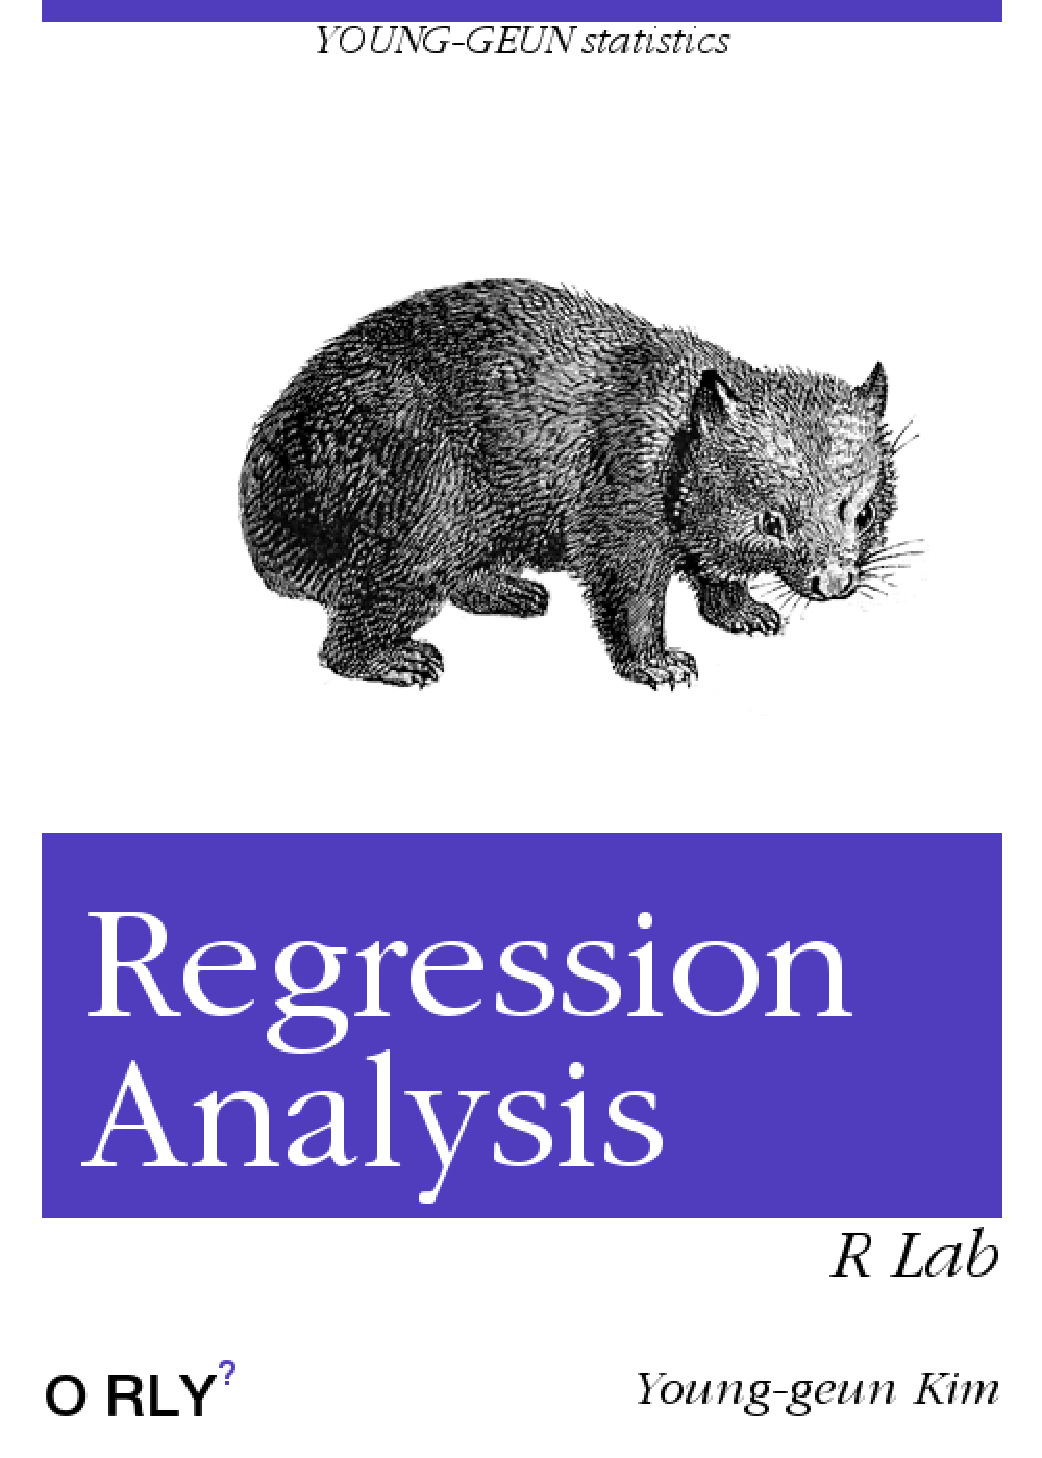
\includepdf{cover.pdf}
\end{titlepage}

\let\maketitle\oldmaketitle
\maketitle

{
\setcounter{tocdepth}{1}
\tableofcontents
}
\hypertarget{welcome}{%
\chapter*{Welcome}\label{welcome}}
\addcontentsline{toc}{chapter}{Welcome}

This book aims at covering materials of regression analysis. Also, there will be R programming for regression.

\begin{Shaded}
\begin{Highlighting}[]
\KeywordTok{library}\NormalTok{(tidyverse)}
\end{Highlighting}
\end{Shaded}

\texttt{tidyverse} package will be used in every chapter, so loading step will be hidden.

\hypertarget{linear-regression-analysis}{%
\section*{Linear Regression Analysis}\label{linear-regression-analysis}}
\addcontentsline{toc}{section}{Linear Regression Analysis}

\begin{Shaded}
\begin{Highlighting}[]
\KeywordTok{data}\NormalTok{(BioOxyDemand, }\DataTypeTok{package =} \StringTok{"MPV"}\NormalTok{)}
\NormalTok{(BioOxyDemand <-}
\StringTok{  }\NormalTok{BioOxyDemand }\OperatorTok\StringTok{ }
\StringTok{  }\KeywordTok{tbl_df}\NormalTok{())}
\CommentTok{#> # A tibble: 14 x 2}
\CommentTok{#>        x     y}
\CommentTok{#>    <int> <int>}
\CommentTok{#>  1     3     4}
\CommentTok{#>  2     8     7}
\CommentTok{#>  3    10     8}
\CommentTok{#>  4    11     8}
\CommentTok{#>  5    13    10}
\CommentTok{#>  6    16    11}
\CommentTok{#>  7    27    16}
\CommentTok{#>  8    30    26}
\CommentTok{#>  9    35    21}
\CommentTok{#> 10    37     9}
\CommentTok{#> 11    38    31}
\CommentTok{#> 12    44    30}
\CommentTok{#> 13   103    75}
\CommentTok{#> 14   142    90}
\end{Highlighting}
\end{Shaded}

\hypertarget{relation}{%
\subsection*{Relation}\label{relation}}
\addcontentsline{toc}{subsection}{Relation}

We wonder how \texttt{x} affects \texttt{y}, especially linearly.

\begin{itemize}
\tightlist
\item
  Functional relation: mathematical equation, \[y = \beta_0 + \beta_1 x\]
\item
  Statistical relation: embeded with noise
\end{itemize}

So we try to estimate

\[y = \beta_0 + \beta_1 x + \epsilon\]

\begin{Shaded}
\begin{Highlighting}[]
\NormalTok{BioOxyDemand }\OperatorTok\StringTok{ }
\StringTok{  }\KeywordTok{ggplot}\NormalTok{(}\KeywordTok{aes}\NormalTok{(x, y)) }\OperatorTok{+}
\StringTok{  }\KeywordTok{geom_point}\NormalTok{()}
\end{Highlighting}
\end{Shaded}

\begin{center}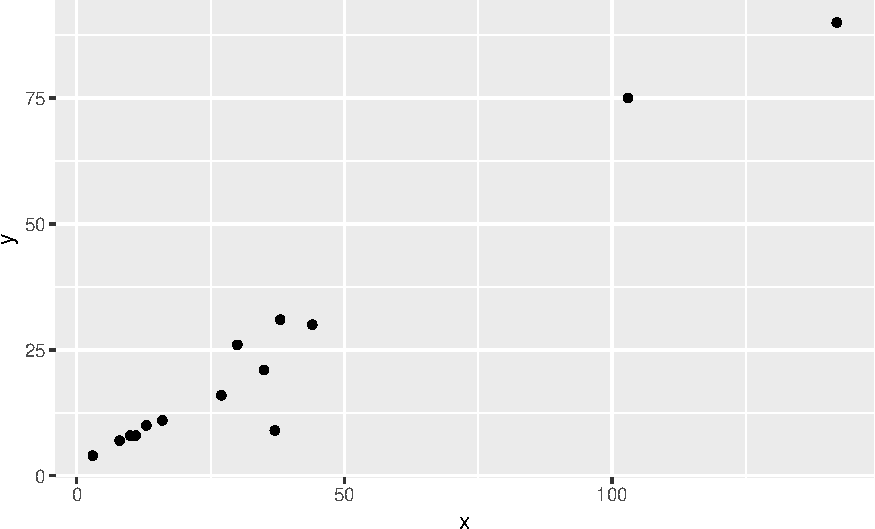
\includegraphics[width=0.7\linewidth]{regression-analysis_files/figure-latex/unnamed-chunk-5-1} \end{center}

Looking just with the eyes, we can see the linear relationship. Regression analysis estimates the relationship statistically.

\begin{Shaded}
\begin{Highlighting}[]
\NormalTok{BioOxyDemand }\OperatorTok\StringTok{ }
\StringTok{  }\KeywordTok{ggplot}\NormalTok{(}\KeywordTok{aes}\NormalTok{(x, y)) }\OperatorTok{+}
\StringTok{  }\KeywordTok{geom_smooth}\NormalTok{(}\DataTypeTok{method =} \StringTok{"lm"}\NormalTok{) }\OperatorTok{+}
\StringTok{  }\KeywordTok{geom_point}\NormalTok{()}
\end{Highlighting}
\end{Shaded}

\begin{center}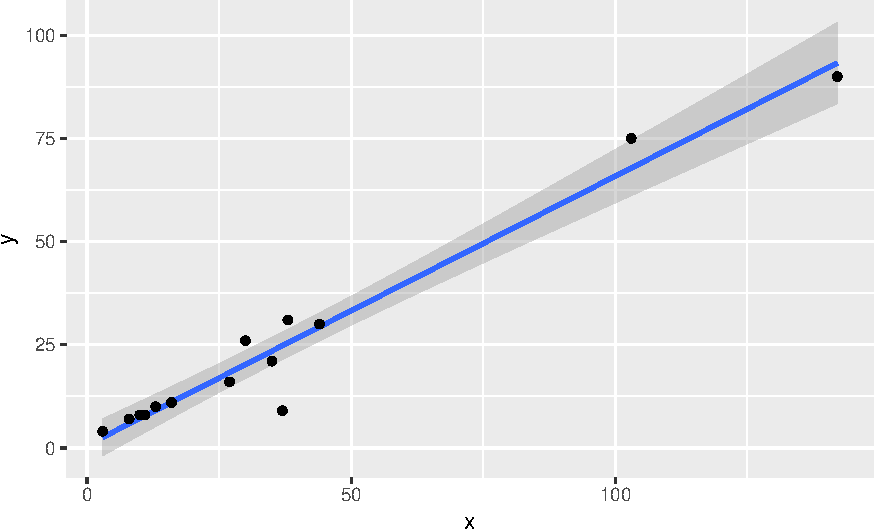
\includegraphics[width=0.7\linewidth]{regression-analysis_files/figure-latex/unnamed-chunk-6-1} \end{center}

\hypertarget{simple}{%
\chapter{Simple Linear Regression}\label{simple}}

\hypertarget{model}{%
\section{Model}\label{model}}

\begin{Shaded}
\begin{Highlighting}[]
\NormalTok{delv <-}\StringTok{ }\NormalTok{MPV}\OperatorTok{::}\NormalTok{p2}\FloatTok{.9} \OperatorTok\StringTok{ }\KeywordTok{tbl_df}\NormalTok{()}
\end{Highlighting}
\end{Shaded}

\begin{Shaded}
\begin{Highlighting}[]
\NormalTok{delv }\OperatorTok\StringTok{ }
\StringTok{  }\KeywordTok{ggplot}\NormalTok{(}\KeywordTok{aes}\NormalTok{(}\DataTypeTok{x =}\NormalTok{ x, }\DataTypeTok{y =}\NormalTok{ y)) }\OperatorTok{+}
\StringTok{  }\KeywordTok{geom_point}\NormalTok{() }\OperatorTok{+}
\StringTok{  }\KeywordTok{labs}\NormalTok{(}
    \DataTypeTok{x =} \StringTok{"Number of Cases"}\NormalTok{,}
    \DataTypeTok{y =} \StringTok{"Delivery Time"}
\NormalTok{  )}
\end{Highlighting}
\end{Shaded}

\begin{figure}[H]

{\centering 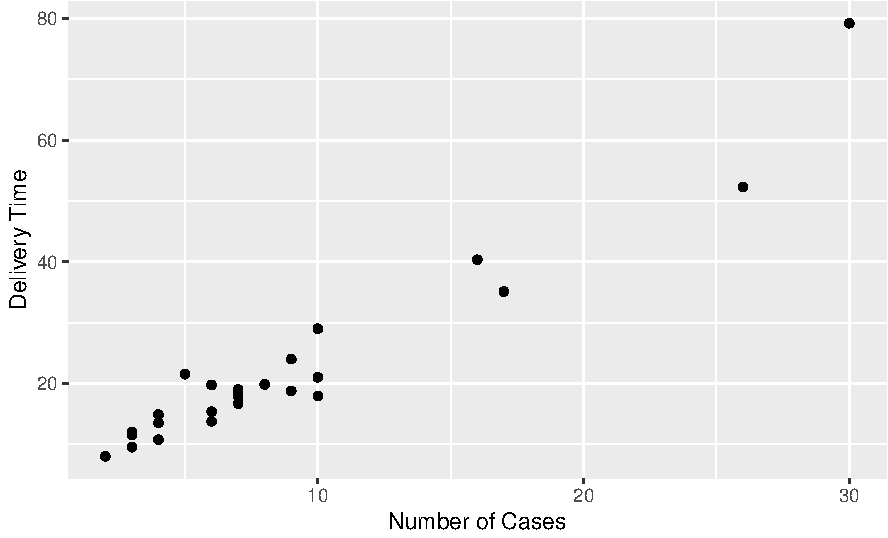
\includegraphics[width=0.7\linewidth]{regression-analysis_files/figure-latex/delivery-1} 

}

\caption{The Delivery Time Data}\label{fig:delivery}
\end{figure}

Given data \((x_1, Y_1), \ldots, (x_n, Y_n)\), we try to fit linear model

\[Y_i = \beta_0 + \beta_1 x_i + \epsilon_i\]

Here \(\epsilon_i\) is a error term, which is a random variable.

\[\epsilon \stackrel{iid}{\sim} (0, \sigma^2)\]

It gives the problem of estimating three parameters \((\beta_0, \beta_1, \sigma^2)\). Before estimating these, we set some assumptions.

\begin{enumerate}
\def\labelenumi{\arabic{enumi}.}
\tightlist
\item
  linear relationship
\item
  \(\epsilon_i\)s are independent
\item
  \(\epsilon_i\)s are identically destributed, i.e.~\emph{constant variance}
\item
  In some setting, \(\epsilon_i \sim N\)
\end{enumerate}

\hypertarget{least-squares-estimation}{%
\section{Least Squares Estimation}\label{least-squares-estimation}}

\begin{figure}[H]

{\centering 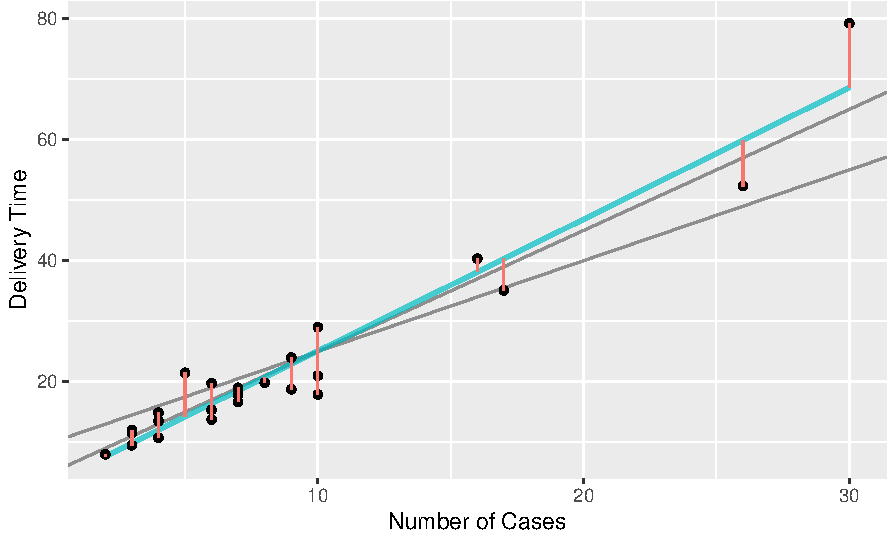
\includegraphics[width=0.7\linewidth]{regression-analysis_files/figure-latex/lsefig-1} 

}

\caption{Idea of the least square estimation}\label{fig:lsefig}
\end{figure}

We try to find \(\beta_0\) and \(\beta_1\) that minimize the sum of squares of the vertical distances, i.e.

\begin{equation}
  (\beta_0, \beta_1) = \arg\min \sum_{i = 1}^n (Y_i - \beta_0 - \beta_1 x_i)^2
  \label{eq:ssq}
\end{equation}

\hypertarget{normal-equations}{%
\subsection{Normal equations}\label{normal-equations}}

Denote that Equation \eqref{eq:ssq} is quadratic. Then we can find its minimum by find the zero point of the first derivative. Set

\[Q(\beta_0, \beta_1) := \sum_{i = 1}^n (Y_i - \beta_0 - \beta_1 x_i)^2\]

Then we have

\begin{equation}
  \frac{\partial Q}{\partial \beta_0} = -2 \sum_{i = 1}^n(Y_i - \beta_0 - \beta_1 x_i) = 0
  \label{eq:normbeta0}
\end{equation}

and

\begin{equation}
  \frac{\partial Q}{\partial \beta_1} = -2 \sum_{i = 1}^n (Y_i - \beta_0 - \beta_1 x_i)x_i = 0
  \label{eq:normbeta1}
\end{equation}

From Equation \eqref{eq:normbeta0},

\[\sum_{i = 1}^n Y_i - n \hat\beta_0 - \hat\beta_1 \sum_{i = 1}^n x_i = 0\]

Thus,

\[\hat\beta_0 = \overline{Y} - \hat\beta_1 \overline{x}\]

Equation \eqref{eq:normbeta1} gives

\[\sum_{i = 1}^n x_i (Y_i - \overline{Y} + \hat\beta_1\overline{x} - \hat\beta_1 x_i) = \sum_{i = 1}^n x_i(Y_i - \overline{Y}) - \hat\beta_1\sum_{i = 1}^n x_i (x_i - \overline{x}) = 0\]

Thus,

\[\hat\beta_1 = \frac{\sum\limits_{i = 1}^nx_i(Y_i - \overline{Y})}{\sum\limits_{i = 1}^n x_i (x_i - \overline{x})}\]

\BeginKnitrBlock{remark}
\iffalse{} {Remark. } \fi{}\[\hat\beta_1 = \frac{S_{XY}}{S_{XX}}\]

where \(S_{XX} := \sum\limits_{i = 1}^n (x_i - \overline{x})^2\) and \(S_{XY} := \sum\limits_{i = 1}^n (x_i - \overline{x})(Y_i - \overline{Y})\)
\EndKnitrBlock{remark}

\BeginKnitrBlock{proof}
\iffalse{} {Proof. } \fi{}Note that \(\overline{x}^2 = \frac{1}{n^2}\bigg(\sum\limits_{i = 1}^n x_i\bigg)^2\). Then we have

\begin{equation}
  \begin{split}
    S_{XX} & = \sum_{i = 1}^n (x_i - \overline{x})^2 \\
    & = \sum_{i = 1}^n x_i^2 - 2\sum_{i = 1}^n x_i \overline{x} + \sum_{i = 1}^n\overline{x}^2 \\
    & = \sum_{i = 1}^n x_i^2 - \frac{2}{n}\bigg(\sum\limits_{i = 1}^n x_i\bigg)^2 + \frac{1}{n}\bigg(\sum\limits_{i = 1}^n x_i\bigg)^2 \\
    & = \sum_{i = 1}^n x_i^2 - \frac{1}{n}\bigg(\sum\limits_{i = 1}^n x_i\bigg)^2
  \end{split}
  \label{eq:sxx}
\end{equation}

It follows that

\begin{equation*}
  \begin{split}
    \hat\beta_1 & = \frac{\sum x_i(Y_i - \overline{Y})}{\sum x_i (x_i - \overline{x})} \\
    & = \frac{\sum x_i (Y_i - \overline{Y}) - \overline{x}\sum (Y_i - \overline{Y})}{\sum x_i^2 - \frac{1}{n} (\sum x_i)^2} \qquad \because \sum (Y_i - \overline{Y}) = 0 \\
    & = \frac{\sum (x_i - \overline{x})(Y_i - \overline{Y})}{\sum x_i^2 - \frac{1}{n} (\sum x_i)^2} \\
    & = \frac{S_{XY}}{S_{XX}}
  \end{split}
\end{equation*}
\EndKnitrBlock{proof}

\begin{Shaded}
\begin{Highlighting}[]
\KeywordTok{lm}\NormalTok{(y }\OperatorTok{~}\StringTok{ }\NormalTok{x, }\DataTypeTok{data =}\NormalTok{ delv)}
\CommentTok{#> }
\CommentTok{#> Call:}
\CommentTok{#> lm(formula = y ~ x, data = delv)}
\CommentTok{#> }
\CommentTok{#> Coefficients:}
\CommentTok{#> (Intercept)            x  }
\CommentTok{#>        3.32         2.18}
\end{Highlighting}
\end{Shaded}

\hypertarget{prediction-and-mean-response}{%
\subsection{Prediction and Mean response}\label{prediction-and-mean-response}}

\begin{quote}
``Essentially, all models are wrong, but some are useful.''

---George Box
\end{quote}

Recall that we have assumed the \textbf{linear assumption} between the predictor and the response variables, i.e.~the true model. Estimating \(\beta_0\) and \(\beta_1\) is same as estimating the \emph{assumed true model}.

\BeginKnitrBlock{definition}[Mean response]
\protect\hypertarget{def:eyx}{}{\label{def:eyx} \iffalse (Mean response) \fi{} }\[E(Y \mid X = x) = \beta_0 + \beta_1 x\]
\EndKnitrBlock{definition}

We can estimate this mean resonse by

\begin{equation}
  \widehat{E(Y \mid x)} = \hat\beta_0 + \hat\beta_1 x
  \label{eq:meanres}
\end{equation}

However, in practice, the model might not be true, which is included in \(\epsilon\) term.

\[Y_i = \beta_0 + \beta_1 x_i + \epsilon_i\]

Our real problem is predicting individual \(Y\), not the mean. The \emph{prediction} of response can be done by

\begin{equation}
  \hat{Y_i}  = \hat\beta_0 + \hat\beta_1 x_i
  \label{eq:indpred}
\end{equation}

Observe that the values of Equations \eqref{eq:meanres} and \eqref{eq:indpred} are same. However, due to the \textbf{error term in the prediction}, it has larger standard error.

\hypertarget{lseprop}{%
\subsection{Properties of LSE}\label{lseprop}}

Parameters \(\beta_0\) and \(\beta_1\) have some properties related to the expectation and variance. We can notice that these lse's are \textbf{unbiased linear estimator}. In fact, these are the \emph{best unbiased linear estimator}. This will be covered in the Gauss-Markov theorem.

\BeginKnitrBlock{lemma}
\protect\hypertarget{lem:sxy}{}{\label{lem:sxy} }\[S_{XX} = \sum_{i = 1}^n x_i^2 - \frac{1}{n}\bigg(\sum\limits_{i = 1}^n x_i\bigg)^2 = \sum_{i = 1}^n x_i(x_i - \overline{x})\]

\[S_{XY} = \sum_{i = 1}^n x_i Y_i - \frac{1}{n}\bigg(\sum_{i = 1}^n x_i\bigg)\bigg(\sum_{i = 1}^n Y_i\bigg) = \sum_{i = 1}^n Y_i(x_i - \overline{x}) = \sum_{i = 1}^n x_i(Y_i - \overline{Y})\]
\EndKnitrBlock{lemma}

\BeginKnitrBlock{proof}
\iffalse{} {Proof. } \fi{}We already proven the first part of \(S_{XX}\). See the Equation \eqref{eq:sxx}. The second part is tivial. Since \(\sum (x_i - \overline{x}) = 0\),

\[S_{XX} = \sum_{i = 1}^n (x_i - \overline{x})^2 = \sum_{i = 1}^n (x_i - \overline{x})x_i\]

For the first part of \(S_{XY}\),

\begin{equation*}
  \begin{split}
    S_{XY} & = \sum_{i = 1}^n (x_i - \overline{x})(Y_i - \overline{Y}) \\
    & = \sum_{i = 1}^n x_i Y_i - \overline{x} \sum_{i = 1}^n Y_i - \overline{Y} \sum_{i = 1}^n x_i + n \overline{x} \overline{Y} \\
    & = \sum_{i = 1}^n x_i Y_i - \frac{1}{n}\bigg(\sum_{i = 1}^n x_i\bigg)\bigg(\sum_{i = 1}^n Y_i\bigg)
  \end{split}
\end{equation*}

Second part of \(S_{XY}\) also can be proven from the definition.

\begin{equation*}
  \begin{split}
    S_{XY} & = \sum_{i = 1}^n (x_i - \overline{x})(Y_i - \overline{Y}) \\
    & = \sum_{i = 1}^n Y_i (x_i - \overline{x}) - \overline{Y} \sum_{i = 1}^n (x_i - \overline{x}) \\
    & = \sum_{i = 1}^n Y_i (x_i - \overline{x}) \qquad \because \sum_{i = 1}^n (x_i - \overline{x}) = 0
  \end{split}
\end{equation*}

Same for the last part.
\EndKnitrBlock{proof}

\BeginKnitrBlock{lemma}[Linearity]
\protect\hypertarget{lem:linbet}{}{\label{lem:linbet} \iffalse (Linearity) \fi{} }Each coefficient is a linear estimator.

\[\hat\beta_1 = \sum_{i = 1}^n\frac{(x_i - \overline{x})}{S_{XX}}Y_i\]

\[\hat\beta_0 = \sum_{i = 1}^n \bigg( \frac{1}{n} - \frac{(x_i - \overline{x})\overline{x}}{S_{XX}} \bigg) Y_i\]
\EndKnitrBlock{lemma}

\BeginKnitrBlock{proof}
\iffalse{} {Proof. } \fi{}From lemma \ref{lem:sxy},

\begin{equation*}
  \begin{split}
    \hat\beta_1 & = \frac{S_{XY}}{S_{XX}} \\
    & = \frac{1}{S_{XX}}\sum_{i = 1}^n (x_i - \overline{x}) Y_i
  \end{split}
\end{equation*}

It gives that

\begin{equation*}
  \begin{split}
    \hat\beta_0 & = \overline{Y} - \hat\beta_1 \overline{x} \\
    & = \frac{1}{n}\sum_{i = 1}^n Y_i - \overline{x} \sum_{i = 1}^n\frac{(x_i - \overline{x})}{S_{XX}}Y_i \\
    & = \sum_{i = 1}^n\bigg(\frac{1}{n} - \frac{(x_i - \overline{x})\overline{x}}{S_{XX}} \bigg)Y_i
  \end{split}
\end{equation*}
\EndKnitrBlock{proof}

\BeginKnitrBlock{proposition}[Unbiasedness]
\protect\hypertarget{prp:ue}{}{\label{prp:ue} \iffalse (Unbiasedness) \fi{} }Both coefficients are unbiased.

\begin{enumerate}
  \item $E\hat\beta_1 = \beta_1$
  \item $E\hat\beta_0 = \beta_0$
\end{enumerate}
\EndKnitrBlock{proposition}

From the model, \(Y_1, \ldots, Y_n \stackrel{indep}{\sim} (\beta_0 + \beta_1 x_i, \sigma^2)\).

\BeginKnitrBlock{proof}
\iffalse{} {Proof. } \fi{}From lemma \ref{lem:sxy},

\begin{equation*}
  \begin{split}
    E\hat\beta_1 & = \sum_{i = 1}^n \bigg[ \frac{(x_i - \overline{x})}{S_{XX}} E(Y_i) \bigg] \\
    & = \sum_{i = 1}^n \frac{(x_i - \overline{x})}{S_{XX}}(\beta_0 + \beta_1 x_i) \\
    & = \frac{\beta_1 \sum (x_i - \overline{x})x_i}{\sum (x_i - \overline{x})x_i} \qquad \because \sum (x_i - \overline{x}) = 0 \\
    & = \beta_1
  \end{split}
\end{equation*}

It follows that

\begin{equation*}
  \begin{split}
    E\hat\beta_0 & = E(\overline{Y} - \hat\beta_1 \overline{x}) \\
    & = E(\overline{Y}) - \overline{x}E(\hat\beta_1) \\
    & = E(\beta_0 + \beta_1 \overline{x} + \overline{\epsilon}) - \beta_1 \overline{x} \\
    & = \beta_0 + \beta_1 \overline{x} - \beta_1 \overline{x} \\
    & = \beta_0
  \end{split}
\end{equation*}
\EndKnitrBlock{proof}

\BeginKnitrBlock{proposition}[Variances]
\protect\hypertarget{prp:vb}{}{\label{prp:vb} \iffalse (Variances) \fi{} }Variances and covariance of coefficients

\begin{enumerate}[label=(\alph*)]
  \item $Var\hat\beta_1 = \frac{\sigma^2}{S_{XX}}$ \label{itm:vbone}
  \item $Var\hat\beta_0 = \bigg( \frac{1}{n} + \frac{\overline{x}^2}{S_{XX}} \bigg)\sigma^2$ \label{itm:vbtwo}
  \item $Cov(\hat\beta_0, \hat\beta_1) = - \frac{\overline{x}}{S_{XX}} \sigma^2$ \label{itm:vbthree}
\end{enumerate}
\EndKnitrBlock{proposition}

\BeginKnitrBlock{proof}
\iffalse{} {Proof. } \fi{}Proving is just arithmetic.

\(\ref{itm:vbone}\)

\begin{equation*}
  \begin{split}
    Var\hat\beta_1 & = \frac{1}{S_{XX}^2}\sum_{i = 1}^n \bigg[ (x_i - \overline{x})^2 Var(Y_i) \bigg] + \frac{1}{S_{XX}^2} \sum_{j \neq k}^n \bigg[ (x_j - \overline{x})(x_k - \overline{x}) Cov(Y_j, Y_k) \bigg] \\
    & = \frac{\sigma^2}{S_{XX}} \qquad \because Cov(Y_j, Y_k) = 0 \: \text{if} \: j \neq k
  \end{split}
\end{equation*}

\(\ref{itm:vbtwo}\)

\begin{equation*}
  \begin{split}
    Var\hat\beta_0 & = \sum_{i = 1}^n \bigg( \frac{1}{n} - \frac{(x_i - \overline{x})\overline{x}}{S_{XX}} \bigg)^2Var(Y_i) + \sum_{j \neq k} \bigg( \frac{1}{n} - \frac{(x_j - \overline{x})\overline{x}}{S_{XX}} \bigg)\bigg( \frac{1}{n} - \frac{(x_k - \overline{x})\overline{x}}{S_{XX}} \bigg) Cov(Y_j, Y_k) \\
    & = \frac{\sigma^2}{n} - 2 \sigma^2 \frac{\overline{x}}{S_{XX}} \sum_{i = 1}^n (x_i - \overline{x}) + \frac{\sigma^2 \overline{x}^2 \sum (x_i - \overline{x})^2}{S_{XX}^2} \\
    & = \bigg( \frac{1}{n} + \frac{\overline{x}^2}{S_{XX}} \bigg) \sigma^2 \qquad \because \sum (x_i - \overline{x}) = 0
  \end{split}
\end{equation*}

\(\ref{itm:vbthree}\)

\begin{equation*}
  \begin{split}
    Cov(\hat\beta_0, \hat\beta_1) & = Cov(\overline{Y} - \hat\beta_1 \overline{x}, \hat\beta_1) \\
    & = - \overline{x} Var\hat\beta_1 \\
    & = - \frac{\overline{x}}{S_{XX}} \sigma^2
  \end{split}
\end{equation*}
\EndKnitrBlock{proof}

\hypertarget{gauss-markov-theorem}{%
\subsection{Gauss-Markov Theorem}\label{gauss-markov-theorem}}

Chapter \ref{lseprop} shows that the \(\beta_0^{LSE}\) and \(\beta_1^{LSE}\) are the \textbf{linear unbiased estimators}. Are these good? Good compared to \emph{what estimators}? Here we consider \emph{linear unbiased estimator}. If variances in the proposition \ref{prp:vb} are lower than any parameters in this parameter family, \(\beta_0^{LSE}\) and \(\beta_1^{LSE}\) are the \textbf{best linear unbiased estimators}.

\BeginKnitrBlock{theorem}[Gauss Markov Theorem]
\protect\hypertarget{thm:gmt}{}{\label{thm:gmt} \iffalse (Gauss Markov Theorem) \fi{} }\(\hat\beta_0\) and \(\hat\beta_1\) are BLUE, i.e.~the best linear unbiased estimator.

\[Var(\hat\beta_0) \le Var\Big( \sum_{i = 1}^n a_i Y_i \Big) \: \forall a_i \in \mathbb{R} \: \text{s.t.} \: E\Big( \sum_{i = 1}^n a_i Y_i \Big) = \beta_0\]

\[Var(\hat\beta_1) \le Var\Big( \sum_{i = 1}^n b_i Y_i \Big) \: \forall b_i \in \mathbb{R} \: \text{s.t.} \: E\Big( \sum_{i = 1}^n b_i Y_i \Big) = \beta_1\]
\EndKnitrBlock{theorem}

\BeginKnitrBlock{proof}[Bestness of $\beta_1$]
\iffalse{} {Proof (Bestness of \(\beta_1\)). } \fi{}Consider \(\Theta := \bigg\{ \sum\limits_{i = 1}^n b_i Y_i \in \mathbb{R} : E\Big( \sum\limits_{i = 1}^n b_i Y_i \Big) = \beta_1 \bigg\}\).

Claim: \(Var( \sum b_i Y_i) - Var(\hat\beta_1) \ge 0\)

Let \(\sum b_i Y_i \in \Theta\). Then \(E(\sum b_i Y_i) = \beta_1\).

Since \(E(Y_i) = \beta_0 + \beta_1 x_i\),

\[\beta_0 \sum b_i + \beta_1 \sum b_i x_i = \beta_1\]

It gives

\begin{equation} \label{eq:ule}
  \begin{cases}
    \sum b_i = 0 \\
    \sum b_i x_i = 1
  \end{cases}
\end{equation}

Then

\begin{equation*}
  \begin{split}
    0 \le Var\Big(\sum b_i Y_i - \hat\beta_1\Big) & = Var\Big( \sum b_i Y_i - \sum \frac{(x_i - \bar{x})}{S_{XX}} Y_i \Big) \\
    & \stackrel{indep}{=} \sum \bigg( b_i - \frac{(x_i - \bar{x})}{S_{XX}} \bigg)^2 \sigma^2 \\
    & = \sum \bigg( b_i^2 - \frac{2b_i (x_i - \bar{x})}{S_{XX}} + \frac{(x_i - \bar{x})^2}{S_{XX}^2} \bigg) \sigma^2 \\
    & = \sum b_i^2 \sigma^2 - \frac{2 \sigma^2}{S_{XX}} \sum b_i x_i + \frac{2 \bar{x} \sigma^2}{S_{XX}} \sum b_i + \sigma^2 \frac{\sum (x_i - \bar{x})^2}{S_{XX}^2} \\
    & = \sum b_i^2 \sigma^2 - \frac{\sigma^2}{S_{XX}} \qquad \because \eqref{eq:ule} \:\text{and}\: S_{XX} = \sum (x_i - \bar{x})^2 \\
    & = Var(\sum b_i Y_i) - Var(\hat\beta_1)
  \end{split}
\end{equation*}

Hence,

\[Var(\sum b_i Y_i) \ge Var(\hat\beta_1)\]
\EndKnitrBlock{proof}

\BeginKnitrBlock{proof}[Bestness of $\beta_0$]
\iffalse{} {Proof (Bestness of \(\beta_0\)). } \fi{}Consider \(\Theta := \bigg\{ \sum\limits_{i = 1}^n a_i Y_i \in \mathbb{R} : E\Big( \sum\limits_{i = 1}^n a_i Y_i \Big) = \beta_0 \bigg\}\).

Claim: \(Var( \sum a_i Y_i) - Var(\hat\beta_0) \ge 0\)

Let \(\sum a_i Y_i \in \Theta\). Then \(E(\sum a_i Y_i) = \beta_0\).

Since \(E(Y_i) = \beta_0 + \beta_1 x_i\),

\[\beta_0 \sum a_i + \beta_1 \sum a_i x_i = \beta_0\]

It gives

\begin{equation} \label{eq:ule0}
  \begin{cases}
    \sum a_i = 1 \\
    \sum a_i x_i = 0
  \end{cases}
\end{equation}

Then

\begin{equation*}
  \begin{split}
    0 \le Var\Big(\sum a_iY_i - \hat\beta_0 \Big) & = Var\bigg[\sum a_iY_i - \sum\Big( \frac{1}{n} - \frac{(x_k - \bar{x})\bar{x}}{S_{XX}} \Big) Y_k \bigg] \\
    & = \sum \bigg(a_i - \frac{1}{n} +  \frac{(x_i - \bar{x})\bar{x}}{S_{XX}} \bigg)^2\sigma^2 \\
    & = \sum \bigg[ a_i^2 - 2a_i\Big( \frac{1}{n} - \frac{(x_i - \bar{x})\bar{x}}{S_{XX}} \Big) + \Big( \frac{1}{n} - \frac{(x_i - \bar{x})\bar{x}}{S_{XX}} \Big)^2 \bigg]\sigma^2 \\
        & = \sum a_i^2\sigma^2 -\frac{2\sigma^2}{n}\sum a_i + \frac{2\bar{x}\sigma^2\sum a_ix_i}{S_{XX}} - \frac{2\bar{x}^2\sigma^2\sum a_i}{S_{XX}} \\
        & \qquad + \sigma^2\bigg( \frac{1}{n} - \frac{2\bar{x}}{nS_{XX}} \sum(x_i - \bar{x}) + \frac{\bar{x}^2\sum(x_i - \bar{x})^2}{S_{XX}^2} \bigg) \\
        & = \sum a_i^2\sigma^2 -\frac{2\sigma^2}{n} - \frac{2\bar{x}^2\sigma^2}{S_{XX}} \qquad \because \eqref{eq:ule0} \\
        & \qquad + \bigg(\frac{1}{n} + \frac{\bar{x}^2}{S_{XX}} \bigg)\sigma^2 \qquad \because \sum(x_i - \bar{x}) = 0 \: \text{and} \: S_{XX} := \sum (x_i - \bar{x})^2 \\
        & = \sum a_i^2\sigma^2 - \bigg( \frac{1}{n} + \frac{\bar{x}^2}{S_{XX}} \bigg)\sigma^2 \\
        & = Var\Big( \sum a_i Y_i \Big) - Var\hat\beta_0
  \end{split}
\end{equation*}

Hence,

\[Var(\sum a_i Y_i) \ge Var(\hat\beta_0)\]
\EndKnitrBlock{proof}

\BeginKnitrBlock{example}
\protect\hypertarget{exm:usingnormal}{}{\label{exm:usingnormal} }Show that \(\sum (Y_i - \hat{Y_i}) = 0\), \(\sum x_i (Y_i - \hat{Y_i}) = 0\), and \(\sum \hat{Y_i} (Y_i - \hat{Y_i}) = 0\).
\EndKnitrBlock{example}

\BeginKnitrBlock{solution}
\iffalse{} {Solution. } \fi{}Consider the two normal equations \eqref{eq:normbeta0} and \eqref{eq:normbeta1}. Note that \(\hat{Y_i} = \hat\beta_0 + \hat\beta_1 x_i\).

From the Equation \eqref{eq:normbeta0}, we have \(\sum (Y_i - \hat{Y_i}) = 0\).

From the Equation \eqref{eq:normbeta1}, we have \(\sum x_i (Y_i - \hat{Y_i}) = 0\).

It follows that

\begin{equation*}
  \begin{split}
    \sum \hat{Y_i} (Y_i - \hat{Y_i}) & = \sum (\hat\beta_0 + \hat\beta_1 x_i) (Y_i - \hat{Y_i}) \\
    & = \hat\beta_0 \sum (Y_i - \hat{Y_i}) + \hat\beta_1 \sum x_i (Y_i - \hat{Y_i}) \\
    & = 0
  \end{split}
\end{equation*}
\EndKnitrBlock{solution}

\hypertarget{estimation-of-sigma2}{%
\subsection{\texorpdfstring{Estimation of \(\sigma^2\)}{Estimation of \textbackslash sigma\^{}2}}\label{estimation-of-sigma2}}

There is the last parameter, \(\sigma^2 = Var(Y_i)\). In the \emph{least squares estimation literary}, we estimate \(\sigma^2\) by

\begin{equation}
  \hat\sigma^2 = \frac{1}{n - 2} \sum_{i = 1}^n (Y_i - \hat\beta_0 - \hat\beta_1 x_i)^2
  \label{eq:siglse}
\end{equation}

Why \(n - 2\)? This makes the estimator unbiased.

\BeginKnitrBlock{proposition}[Unbiasedness]
\protect\hypertarget{prp:sigex}{}{\label{prp:sigex} \iffalse (Unbiasedness) \fi{} }\[E(\hat\sigma^2) = \sigma^2\]
\EndKnitrBlock{proposition}

\BeginKnitrBlock{proof}
\iffalse{} {Proof. } \fi{}Note that

\[(Y_i - \hat\beta_0 - \hat\beta_1 x_i) = (Y_i - \overline{Y}) - \hat\beta_1(x_i - \overline{x})\]

Then

\begin{equation*}
  \begin{split}
    E(\hat\sigma^2) & = \frac{1}{n - 2} E \bigg[ \sum (Y_i - \hat\beta_0 - \hat\beta_1 x_i)^2 \bigg] \\
    & = \frac{1}{n - 2} E \bigg[ \sum (Y_i - \overline{Y})^2 + \hat\beta_1^2 \sum (x_i - \overline{x})^2 -2\hat\beta_1 \sum (Y_i - \overline{Y})(x_i - \overline{x}) \bigg] \\
    & = \frac{1}{n - 2} E ( S_{YY} + \hat\beta_1^2 S_{XX} - 2 \hat\beta_1 S_{XY}) \\
    & = \frac{1}{n - 2} E ( S_{YY} - \hat\beta_1^2 S_{XX}) \qquad \because S_{XY} = \hat\beta_1 S_{XX} \\
    & = \frac{1}{n - 2} \Big(  \underset{(a)}{\underline{ES_{YY}}} - S_{XX} \underset{(b)}{\underline{E\hat\beta_1^2}} \Big)
  \end{split}
\end{equation*}

\begin{enumerate}
\def\labelenumi{(\alph{enumi})}
\item
\end{enumerate}

\begin{equation*}
  \begin{split}
    ES_{YY} & = E\Big[ \sum (Y_i - \overline{Y})^2 \Big] \\
    & = E \Big[ \sum \Big( (\beta_0 + \beta_1 x_i + \epsilon_i) - (\beta_0 + \beta_1 \overline{x} + \overline{\epsilon}) \Big)^2 \Big] \\
    & = E \Big[ \sum \Big( \beta_1 (x_i - \overline{x}) + (\epsilon_i - \overline{\epsilon}) \Big)^2 \Big] \\
    & = \beta_1^2 S_{XX} + E\Big( \sum (\epsilon_i - \overline{\epsilon})^2 \Big) + 2\beta_1 \sum (x_i - \overline{x}) E(\epsilon_i - \overline{\epsilon}) \\
    & = \beta_1^2 S_{XX} + E\Big( \sum (\epsilon_i - \overline{\epsilon})^2 \Big)
  \end{split}
\end{equation*}

Since \(E(\bar\epsilon) = 0\) and \(Var(\bar\epsilon) = \frac{\sigma^2}{n}\),

\begin{equation*}
  \begin{split}
    E\Big( \sum (\epsilon_i - \overline{\epsilon})^2 \Big) & = E \Big( \sum (\epsilon_i^2 + \bar\epsilon^2 - 2\epsilon_i \bar\epsilon) \Big) \\
    & = \sum E(\epsilon_i^2) - n E(\bar\epsilon^2) \qquad \because \sum \epsilon = n \bar\epsilon \\
    & = \sum (Var(\epsilon_i) + E(\epsilon_i)^2) - n(Var(\bar\epsilon) + E(\bar\epsilon)^2) \\
    & = n\sigma^2 - \sigma^2 \\
    & = (n - 1)\sigma^2
  \end{split}
\end{equation*}

Thus,

\[ES_{YY} = \beta_1^2 S_{XX} + (n - 1)\sigma^2\]

\begin{enumerate}
\def\labelenumi{(\alph{enumi})}
\setcounter{enumi}{1}
\item
\end{enumerate}

\begin{equation*}
  \begin{split}
    E\hat\beta_1^2 & = Var\hat\beta_1 + E(\hat\beta_1)^2 \\
    & = \frac{\sigma^2}{S_{XX}} + \beta_1^2
  \end{split}
\end{equation*}

It follows that

\begin{equation*}
  \begin{split}
    E(\hat\sigma^2) & = \frac{1}{n - 2} \Big(  \underset{(a)}{\underline{ES_{YY}}} - S_{YY} \underset{(b)}{\underline{E\hat\beta_1^2}} \Big) \\
    & = \frac{1}{n - 2} \bigg( \Big(\beta_1^2 S_{XX} + (n - 1)\sigma^2 \Big) - S_{XX}\Big(\frac{\sigma^2}{S_{XX}} + \beta_1^2 \Big) \bigg) \\
    & = \frac{1}{n - 2}((n - 2)\sigma^2) \\
    & = \sigma^2
  \end{split}
\end{equation*}
\EndKnitrBlock{proof}

\hypertarget{maximum-likelihood-estimation}{%
\section{Maximum Likelihood Estimation}\label{maximum-likelihood-estimation}}

In this section, we add an assumption to an random errors \(\epsilon_i\).

\[\epsilon_i \stackrel{iid}{\sim} N(0, \sigma^2)\]

\BeginKnitrBlock{example}[Gaussian Likelihood]
\protect\hypertarget{exm:gmle}{}{\label{exm:gmle} \iffalse (Gaussian Likelihood) \fi{} }Note that \(Y_i \stackrel{indep}{\sim} N(\beta_0 + \beta_1 x_i, \sigma^2)\). Then the likelihood function is

\[L(\beta_0, \beta_1, \sigma^2) = \prod_{i = 1}^n\bigg( \frac{1}{\sqrt{2\pi\sigma^2}} \exp \bigg(- \frac{(Y_i - \beta_0 - \beta_1 x_i)^2}{2 \sigma^2} \bigg) \bigg)\]

and so the log-likelihood function can be computed as

\[l(\beta_0, \beta_1, \sigma^2) = -\frac{n}{2}\ln(2\pi\sigma^2) - \frac{1}{2\sigma^2}\sum_{i = 1}^n(Y_i - \beta_0 - \beta_1 x_i)^2\]
\EndKnitrBlock{example}

\hypertarget{likelihood-equations}{%
\subsection{Likelihood equations}\label{likelihood-equations}}

\BeginKnitrBlock{definition}[Maximum Likelihood Estimator]
\protect\hypertarget{def:mledef}{}{\label{def:mledef} \iffalse (Maximum Likelihood Estimator) \fi{} }\[(\hat\beta_0^{MLE}, \hat\beta_1^{MLE}, \hat\sigma^{2MLE}) := \arg\sup L(\beta_0, \beta_1, \sigma^2)\]
\EndKnitrBlock{definition}

Since \(l(\cdot) = \ln L(\cdot)\) is monotone,

\BeginKnitrBlock{remark}
\iffalse{} {Remark. } \fi{}\[(\hat\beta_0^{MLE}, \hat\beta_1^{MLE}, \hat\sigma^{2MLE}) = \arg\sup l(\beta_0, \beta_1, \sigma^2)\]
\EndKnitrBlock{remark}

We can find the maximum of this \emph{quadratic} function by making first derivative.

\begin{equation}
  \frac{\partial l}{\partial \beta_0} = \frac{1}{\sigma^2} \sum_{i = 1}^n (Y_i - \beta_0 - \beta_1 x_i) = 0
  \label{eq:mlbeta0}
\end{equation}

\begin{equation}
  \frac{\partial l}{\partial \beta_1} = \frac{1}{\sigma^2} \sum_{i = 1}^n x_i (Y_i - \beta_0 - \beta_1 x_i) = 0
  \label{eq:mlbeta1}
\end{equation}

\begin{equation}
  \frac{\partial l}{\partial \sigma^2} = - \frac{n}{2\sigma^2} + \frac{1}{2\sigma^4} \sum_{i = 1}^n (Y_i - \beta_0 - \beta_1 x_i)^2 = 0
  \label{eq:mlsig}
\end{equation}

Denote that Equations \eqref{eq:mlbeta0} and \eqref{eq:mlbeta1} given \(\hat\sigma^2\) are equivalent to the normal equations. Thus,

\[\hat\beta_0^{MLE} = \hat\beta_0^{LSE}, \quad \hat\beta_1^{MLE} = \hat\beta_1^{LSE}\]

From Equation \eqref{eq:mlsig},

\[\hat\sigma^{2MLE} = \frac{1}{n}\sum_{i = 1}^n(Y_i - \beta_0 - \beta_1 x_i)^2 = \frac{n - 2}{n} \hat\sigma^{2LSE}\]

While \(\hat\sigma^{2LSE}\) is an unbiased, above \emph{MLE is not an unbiased estimator}. Since \(\hat\sigma^{2MLE} \approx \hat\sigma^{2LSE}\) for large \(n\), howerver, it is \emph{asymptotically unbiased}.

\BeginKnitrBlock{theorem}[Rao-Cramer Lower Bound, univariate case]
\protect\hypertarget{thm:rclb}{}{\label{thm:rclb} \iffalse (Rao-Cramer Lower Bound, univariate case) \fi{} }Let \(X_1, \ldots, X_n \stackrel{iid}{\sim} f(x ; \theta)\). If \(\hat\theta\) is an unbiased estimator of \(\theta\),

\[Var(\hat\theta) \ge \frac{1}{I_n(\theta)}\]

where \(I_n(\theta) = -E\bigg(\frac{\partial^2 l(\theta)}{\partial \theta^2} \bigg)\)
\EndKnitrBlock{theorem}

To apply this theorem \ref{thm:rclb} in the simple linear regression setting, i.e.~\((\beta_0, \beta_1)\), we need to look at the \emph{bivariate case}.

\BeginKnitrBlock{theorem}[Rao-Cramer Lower Bound, bivariate case]
\protect\hypertarget{thm:rclb2}{}{\label{thm:rclb2} \iffalse (Rao-Cramer Lower Bound, bivariate case) \fi{} }Let \(X_1, \ldots, X_n \stackrel{iid}{\sim} f(x ; \theta1, \theta_2)\) and let \(\boldsymbol{\theta} = (\theta_1, \theta_2)^T\). If each \(\hat\theta_1\), \(\hat\theta_2\) is an unbiased estimator of \(\theta_1\) and \(\theta_2\), then

\[
Var(\boldsymbol{\theta}) := \begin{bmatrix}
Var(\hat\theta_1) & Cov(\hat\theta_1, \hat\theta_2) \\
Cov(\hat\theta_1, \hat\theta_2) & Var(\hat\theta_2)
\end{bmatrix} \ge I_n^{-1}(\theta_1, \theta_2)
\]

where

\[
I_n(\theta_1, \theta_2) = - \begin{bmatrix}
  E\bigg( \frac{\partial^2 l(\theta_1, \theta_2)}{\partial \theta_1^2} \bigg) & E\bigg( \frac{\partial^2 l(\theta_1, \theta_2)}{\partial \theta_1 \partial \theta_2} \bigg) \\
  E\bigg( \frac{\partial^2 l(\theta_1, \theta_2)}{\partial \theta_1 \partial \theta_2} \bigg) & E\bigg( \frac{\partial^2 l(\theta_1, \theta_2)}{\partial \theta_2^2} \bigg)
\end{bmatrix}
\]
\EndKnitrBlock{theorem}

Assume that \(\sigma^2\) is \textbf{known}. From the Equations \eqref{eq:mlbeta0} and \eqref{eq:mlbeta1},

\[
\begin{cases}
  \frac{\partial^2 l}{\partial \beta_0^2} = - \frac{n}{\sigma^2} \\
  \frac{\partial^2 l}{\partial \beta_1^2} = - \frac{\sum x_i^2}{\sigma^2} \\
  \frac{\partial^2 l}{\partial \beta_0 \partial \beta_1} = - \frac{\sum x_i}{\sigma^2}
\end{cases}
\]

Thus,

\[
I_n(\beta_0, \beta_1) = \begin{bmatrix}
  \frac{n}{\sigma^2} & \frac{\sum x_i}{\sigma^2} \\
  \frac{\sum x_i}{\sigma^2} & \frac{\sum x_i^2}{\sigma^2}
\end{bmatrix}
\]

Applying gaussian elimination,

\begin{equation*}
  \begin{split}
    \left[
    \begin{array}{cc|cc}
      \frac{n}{\sigma^2} & \frac{\sum x_i}{\sigma^2} & 1 & 0 \\
      \frac{\sum x_i}{\sigma^2} & \frac{\sum x_i^2}{\sigma^2} & 0 & 1
    \end{array}
    \right] & \leftrightarrow \left[
    \begin{array}{cc|cc}
      \frac{n}{\sigma^2} & \frac{\sum x_i}{\sigma^2} & 1 & 0 \\
      \frac{\sum x_i}{\sigma^2}\Big(\frac{n}{\sum x_i} \Big) & \frac{\sum x_i^2}{\sigma^2}\Big(\frac{n}{\sum x_i} \Big) & 0 & \frac{1}{\overline{x}}
    \end{array}
    \right] \\
    & \leftrightarrow \left[
    \begin{array}{cc|cc}
      \frac{n}{\sigma^2} & \frac{\sum x_i}{\sigma^2} & 1 & 0 \\
      0 & \frac{\sum x_i^2 - \overline{x}\sum x_i}{\sigma^2\overline{x}} = \frac{S_{XX}}{\sigma^2\overline{x}} & -1 & \frac{1}{\overline{x}}
    \end{array}
    \right] \\
    & \leftrightarrow \left[
    \begin{array}{cc|cc}
      1 & \overline{x} & \frac{\sigma^2}{n} & 0 \\
      0 & 1 & -\frac{\overline{x}}{S_{XX}}\sigma^2 & \frac{\sigma^2}{S_{XX}}
    \end{array}
    \right] \\
    & \leftrightarrow \left[
    \begin{array}{cc|cc}
      1 & 0 & \bigg(\frac{1}{n} + \frac{\overline{x}^2}{S_{XX}} \bigg)\sigma^2 & -\frac{\overline{x}}{S_{XX}}\sigma^2 \\
      0 & 1 & -\frac{\overline{x}}{S_{XX}}\sigma^2 & \frac{\sigma^2}{S_{XX}}
    \end{array}
    \right]
  \end{split}
\end{equation*}

Hence,

\[
I_n^{-1}(\beta_0, \beta_1) = \begin{bmatrix}
  \bigg(\frac{1}{n} + \frac{\overline{x}^2}{S_{XX}} \bigg)\sigma^2 & -\frac{\overline{x}}{S_{XX}}\sigma^2 \\
  -\frac{\overline{x}}{S_{XX}}\sigma^2 & \frac{\sigma^2}{S_{XX}}
\end{bmatrix} = \begin{bmatrix}
  Var(\hat\beta_0) & Cov(\hat\beta_0, \hat\beta_1) \\
  Cov(\hat\beta_0, \hat\beta_1) & Var(\hat\beta_1)
\end{bmatrix}
\]

Since \(Var(\boldsymbol{\hat\beta}) - I^{-1} = 0\) is non-negative definite, each \(Var(\hat\beta_0) = \bigg(\frac{1}{n} + \frac{\overline{x}^2}{S_{XX}} \bigg)\sigma^2\) and \(Var(\hat\beta_1) = \frac{\sigma^2}{S_{XX}}\) is a theoretical bound.

\BeginKnitrBlock{remark}
\iffalse{} {Remark. } \fi{}This says that \(\hat\beta_0^{LSE} = \hat\beta_0^{MLE}\) and \(\hat\beta_1^{LSE} = \hat\beta_1^{MLE}\) have the smallest variance among all unbiased estimator.
\EndKnitrBlock{remark}

This result is \emph{stronger than Gauss-Markov theorem} \ref{thm:gmt}, where the LSE has the smalleset variance among all \emph{linear unbiased} estimators. It can be simply obtained from the \emph{Lehmann-Scheffe Theorem}: If some unbiased estimator is a function of complete sufficient statistic, then this estimator is the unique MVUE \citep{Hogg:2018aa}.

\BeginKnitrBlock{remark}[Lehmann and Scheffe for regression coefficients]
\iffalse{} {Remark (Lehmann and Scheffe for regression coefficients). } \fi{}\(u\Big(\sum Y_i, S_{XY} \Big)\) is CSS in this regression problem, i.e.~known \(\sigma^2\).
\EndKnitrBlock{remark}

\BeginKnitrBlock{proof}
\iffalse{} {Proof. } \fi{}From the example \ref{exm:gmle},

\begin{equation*}
  \begin{split}
    L(\beta_0, \beta_1) & = (2\pi\sigma^2)^{-\frac{n}{2}}\exp\bigg[-\frac{1}{2\sigma^2} \sum(Y_i - \beta_0 - \beta_1 x_i)^2 \bigg] \\
    & = (2\pi\sigma^2)^{-\frac{n}{2}}\exp\bigg[-\frac{1}{2\sigma^2} \sum \Big(Y_i^2 - (\beta_0 + \beta_1 x_i)Y_i + (\beta_0 + \beta_1 x_i)^2 \Big) \bigg] \\
    & = (2\pi\sigma^2)^{-\frac{n}{2}}\exp\bigg[-\frac{1}{2\sigma^2} \Big( -\beta_0 \sum Y_i - \beta_1 \sum x_i Y_i \Big) \bigg] \exp\bigg[-\frac{1}{2\sigma^2} \Big( \sum Y_i^2 + (\beta_0 + \beta_1 x_i)^2 \Big) \bigg]
  \end{split}
\end{equation*}

By the Factorization theorem, both \(\sum Y_i\) and \(\sum x_i Y_i\) are sufficient statistics. Since \(S_{XY}\) is one-to-one function of \(\sum x_i Y_i\), it is also a sufficient statistic.

Denote that the normal distribution is in exponential family.

Hence, \((\sum Y_i, S_{XY})\) are CSS.
\EndKnitrBlock{proof}

\hypertarget{residuals}{%
\section{Residuals}\label{residuals}}

\BeginKnitrBlock{definition}[Residuals]
\protect\hypertarget{def:res}{}{\label{def:res} \iffalse (Residuals) \fi{} }\[e_i := Y_i - \hat{Y_i}\]
\EndKnitrBlock{definition}

\hypertarget{prediction-error}{%
\subsection{Prediction error}\label{prediction-error}}

\begin{Shaded}
\begin{Highlighting}[]
\NormalTok{delv }\OperatorTok\StringTok{ }
\StringTok{  }\KeywordTok{mutate}\NormalTok{(}\DataTypeTok{yhat =} \KeywordTok{predict}\NormalTok{(}\KeywordTok{lm}\NormalTok{(y }\OperatorTok{~}\StringTok{ }\NormalTok{x))) }\OperatorTok\StringTok{ }
\StringTok{  }\KeywordTok{ggplot}\NormalTok{(}\KeywordTok{aes}\NormalTok{(}\DataTypeTok{x =}\NormalTok{ x, }\DataTypeTok{y =}\NormalTok{ y)) }\OperatorTok{+}
\StringTok{  }\KeywordTok{geom_smooth}\NormalTok{(}\DataTypeTok{method =} \StringTok{"lm"}\NormalTok{, }\DataTypeTok{se =} \OtherTok{FALSE}\NormalTok{) }\OperatorTok{+}
\StringTok{  }\KeywordTok{geom_point}\NormalTok{() }\OperatorTok{+}
\StringTok{  }\KeywordTok{geom_linerange}\NormalTok{(}\KeywordTok{aes}\NormalTok{(}\DataTypeTok{ymin =}\NormalTok{ y, }\DataTypeTok{ymax =}\NormalTok{ yhat), }\DataTypeTok{col =} \KeywordTok{I}\NormalTok{(}\StringTok{"red"}\NormalTok{), }\DataTypeTok{alpha =} \FloatTok{.7}\NormalTok{) }\OperatorTok{+}
\StringTok{  }\KeywordTok{labs}\NormalTok{(}
    \DataTypeTok{x =} \StringTok{"Number of Cases"}\NormalTok{,}
    \DataTypeTok{y =} \StringTok{"Delivery Time"}
\NormalTok{  )}
\end{Highlighting}
\end{Shaded}

\begin{figure}[H]

{\centering 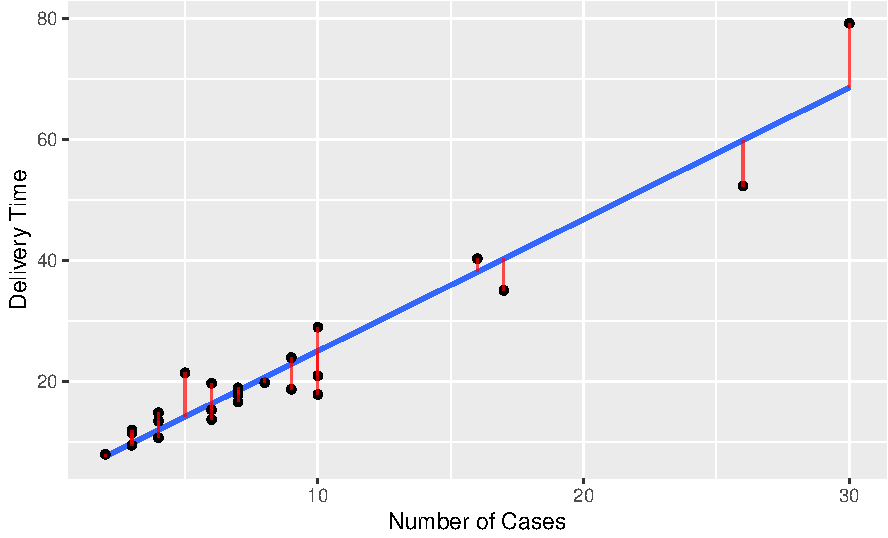
\includegraphics[width=0.7\linewidth]{regression-analysis_files/figure-latex/regplot-1} 

}

\caption{Fit and residuals}\label{fig:regplot}
\end{figure}

See Figure \ref{fig:regplot}. Each red line is \(e_i\). As we can see, \(e_i\) represents the difference between \emph{observed} response and \emph{predicted} response. A large \(\lvert e_i \rvert\) indicates a large prediction error. You can call this \(e_i\) for each \(Y_i\) by \texttt{lm()\$residuals} or \texttt{residuals()}.

\begin{Shaded}
\begin{Highlighting}[]
\NormalTok{delv_fit <-}\StringTok{ }\KeywordTok{lm}\NormalTok{(y }\OperatorTok{~}\StringTok{ }\NormalTok{x, }\DataTypeTok{data =}\NormalTok{ delv)}
\NormalTok{delv_fit}\OperatorTok{$}\NormalTok{residuals}
\CommentTok{#>      1      2      3      4      5      6      7      8      9     10 }
\CommentTok{#> -1.874  1.651  2.181  2.855 -2.628 -0.444  0.327 -0.724 10.634  7.298 }
\CommentTok{#>     11     12     13     14     15     16     17     18     19     20 }
\CommentTok{#>  2.191 -4.082  1.475  3.372  1.094  3.918 -1.028  0.446 -0.349 -5.216 }
\CommentTok{#>     21     22     23     24     25 }
\CommentTok{#> -7.182 -7.581 -4.156 -0.900 -1.275}
\end{Highlighting}
\end{Shaded}

\(\sum e_i^2\), which has been minimized in the procedure of LSE, can be used to see \emph{overall size of prediction errors}.

\BeginKnitrBlock{definition}[Residual Sum of Squares]
\protect\hypertarget{def:sse}{}{\label{def:sse} \iffalse (Residual Sum of Squares) \fi{} }\[SSE := \sum_{i = 1}^n e_i^2\]
\EndKnitrBlock{definition}

\hypertarget{residuals-and-the-variance}{%
\subsection{Residuals and the variance}\label{residuals-and-the-variance}}

\(e_i\) is a random quantity, which contains the information for \(\epsilon_i\). \(\sum e_i^2\) can give information about \(\sigma^2 = Var(\epsilon_i)\). For this, it is expected that \(e_i\) and \(\epsilon_i\) have similar feature.

\BeginKnitrBlock{lemma}
\protect\hypertarget{lem:yandbet}{}{\label{lem:yandbet} }Covriance between Y and each coefficient

\begin{enumerate}[label=(\alph*)]
  \item $Cov(\hat\beta_0, Y_i) = \bigg( \frac{1}{n} - \frac{(x_i - \overline{x})\overline{x}}{S_{XX}} \bigg)\sigma^2$ \label{itm:yandbetone}
  \item $Cov(\hat\beta_1, Y_i) = \frac{(x_i - \overline{x})}{S_{XX}}\sigma^2$ \label{itm:yandbettwo}
\end{enumerate}
\EndKnitrBlock{lemma}

\BeginKnitrBlock{proof}
\iffalse{} {Proof. } \fi{}\(\ref{itm:yandbetone}\)

\begin{equation*}
  \begin{split}
    Cov(\hat\beta_0, Y_i) & = Cov(\sum a_i Y_i, Y_i) \\
    & = \bigg( \frac{1}{n} - \frac{(x_i - \overline{x})\overline{x}}{S_{XX}} \bigg)\sigma^2
  \end{split}
\end{equation*}

\(\ref{itm:yandbettwo}\)

\begin{equation*}
  \begin{split}
    Cov(\hat\beta_1, Y_i) & = Cov(\sum b_i Y_i, Y_i) \\
    & = \frac{(x_i - \overline{x})}{S_{XX}}\sigma^2
  \end{split}
\end{equation*}
\EndKnitrBlock{proof}

\BeginKnitrBlock{proposition}[Properties of residuals]
\protect\hypertarget{prp:resprop}{}{\label{prp:resprop} \iffalse (Properties of residuals) \fi{} }Mean and variance of the residual

\begin{enumerate}[label=(\alph*)]
  \item $E(e_i) = 0$ \label{itm:respropone}
  \item $Var(e_i) \neq \sigma^2$ \label{itm:resproptwo}
  \item $\forall i \neq j : Cov(e_i, e_j) \neq 0$ \label{itm:respropthree}
\end{enumerate}
\EndKnitrBlock{proposition}

\BeginKnitrBlock{proof}
\iffalse{} {Proof. } \fi{}\(\ref{itm:respropone}\) Recall that this is the assumption of the regression model.

\(\ref{itm:resproptwo}\) Lemma \ref{lem:yandbet} implies that

\begin{equation*}
  \begin{split}
    Cov(\overline{Y}, \hat\beta_1) & = Cov(\frac{1}{n}\sum Y_i, \hat\beta_1) \\
    & = \frac{1}{n} \sum_{i = 1}^n \frac{(x_i - \overline{x})}{S_{XX}}\sigma^2 \\
    & = 0 \qquad \because \sum (x_i - \overline{x}) = 0
  \end{split}
\end{equation*}

Then

\begin{equation}
  \begin{split}
    Var(\hat{Y_i}) & = Var(\hat\beta_0 + \hat\beta_1 x_i) \\
    & = Var \bigg[ \overline{Y} + (x_i - \overline{x}) \hat\beta_1 \bigg] \qquad \because \hat\beta_0 = \overline{Y} - \hat\beta_1 \overline{x} \\
    & = Var(\overline{Y}) + (x_i - \overline{x})^2 Var(\hat\beta_1) + 2(x_i - \overline{x}) Cov(\overline{Y}, \hat\beta_1) \\
    & = \frac{\sigma^2}{n} + (x_i - \overline{x})^2\frac{\sigma^2}{S_{XX}} + 0 \\
    & = \bigg( \frac{1}{n} + \frac{(x_i - \overline{x})^2}{S_{XX}} \bigg)\sigma^2
  \end{split}
  \label{eq:predvar}
\end{equation}

From the same lemma \ref{lem:yandbet},

\begin{equation}
  \begin{split}
    Cov(Y_i, \hat{Y_i}) & = Cov(Y_i, \overline{Y} + (x_i - \overline{x}) \hat\beta_1) \\
    & = Cov(Y_i, \overline{Y}) + (x_i - \overline{x}) Cov(Y_i, \hat\beta_1) \\
    & = \frac{\sigma^2}{n} + \frac{(x_i - \overline{x})^2}{S_{XX}}\sigma^2 \qquad \because Cov(Y_i, \hat\beta_1) = \frac{(x_i - \overline{x})}{S_{XX}}\sigma^2 \\
    & = \bigg( \frac{1}{n} + \frac{(x_i - \overline{x})^2}{S_{XX}} \bigg)\sigma^2
  \end{split}
  \label{eq:yyhat}
\end{equation}

These Equations \eqref{eq:predvar} and \eqref{eq:yyhat} give that

\begin{equation}
  \begin{split}
    Var(e_i) & = Var(Y_i) + Var(\hat{Y_i}) -2Cov(Y_i, \hat{Y_i}) \\
    & = \sigma^2 + \bigg( \frac{1}{n} + \frac{(x_i - \overline{x})^2}{S_{XX}} \bigg)\sigma^2 - 2 \bigg( \frac{1}{n} + \frac{(x_i - \overline{x})^2}{S_{XX}} \bigg)\sigma^2 \\
    & = \bigg(1 - \frac{1}{n} - \frac{(x_i - \overline{x})^2}{S_{XX}} \bigg)\sigma^2 \\
    & \neq \sigma^2
  \end{split}
  \label{eq:residvar}
\end{equation}

\(\ref{itm:respropthree}\) Let \(i \neq j\). Then

\begin{equation*}
  \begin{split}
    Cov(e_i, e_j) & = Cov\Big( Y_i - (\hat\beta_0 + \hat\beta_1 x_i), Y_j - (\hat\beta_0 + \hat\beta_1 x_j) \Big) \\
    & = Cov(Y_i, Y_j) - Cov\Big(Y_i, (\hat\beta_0 + \hat\beta_1 x_j) \Big) - Cov((\hat\beta_0 + \hat\beta_1 x_i), Y_j) + Cov((\hat\beta_0 + \hat\beta_1 x_i), (\hat\beta_0 + \hat\beta_1 x_j)) \\
    & = 0 - \bigg( \frac{1}{n} - \frac{(x_i - \overline{x})\overline{x}}{S_{XX}} \bigg)\sigma^2 - \frac{(x_i - \overline{x})x_j}{S_{XX}}\sigma^2 \\
    & \qquad - \bigg( \frac{1}{n} - \frac{(x_j - \overline{x})\overline{x}}{S_{XX}} \bigg)\sigma^2 - \frac{(x_i - \overline{x})x_i}{S_{XX}}\sigma^2 \\
    & \qquad + \bigg( \frac{1}{n} + \frac{\overline{x}^2 + x_i x_j - \overline{x}(x_i + x_j)}{S_{XX}} \bigg)\sigma^2 \\
    & = - \bigg( \frac{1}{n} + \frac{\overline{x}^2 + x_i x_j - \overline{x}(x_i + x_j)}{S_{XX}} \bigg)\sigma^2 \\
    & = - \bigg( \frac{1}{n} + \frac{(x_i - \overline{x})(x_j - \overline{x})}{S_{XX}} \bigg)\sigma^2 \\
    & \neq 0
  \end{split}
\end{equation*}
\EndKnitrBlock{proof}

\hypertarget{decomposition-of-total-variability}{%
\section{Decomposition of Total Variability}\label{decomposition-of-total-variability}}

\hypertarget{total-sum-of-squares}{%
\subsection{Total sum of squares}\label{total-sum-of-squares}}

\BeginKnitrBlock{definition}[Uncorrected Total Sum of Squares]
\protect\hypertarget{def:unsst}{}{\label{def:unsst} \iffalse (Uncorrected Total Sum of Squares) \fi{} }\[SST_{uncor} := \sum_{i = 1}^n Y_i^2\]
\EndKnitrBlock{definition}

\BeginKnitrBlock{definition}[Corrected Total Sum of Squares]
\protect\hypertarget{def:sst}{}{\label{def:sst} \iffalse (Corrected Total Sum of Squares) \fi{} }\[SST := \sum_{i = 1}^n (Y_i - \overline{Y})^2\]
\EndKnitrBlock{definition}

What does this total sum of squares mean? To know this, we should know \(\overline{Y}\) first.

\begin{Shaded}
\begin{Highlighting}[]
\NormalTok{delv }\OperatorTok\StringTok{ }
\StringTok{  }\KeywordTok{ggplot}\NormalTok{(}\KeywordTok{aes}\NormalTok{(}\DataTypeTok{x =}\NormalTok{ x, }\DataTypeTok{y =}\NormalTok{ y)) }\OperatorTok{+}
\StringTok{  }\KeywordTok{geom_smooth}\NormalTok{(}\DataTypeTok{method =} \StringTok{"lm"}\NormalTok{, }\DataTypeTok{formula =}\NormalTok{ y }\OperatorTok{~}\StringTok{ }\DecValTok{1}\NormalTok{, }\DataTypeTok{se =} \OtherTok{FALSE}\NormalTok{) }\OperatorTok{+}
\StringTok{  }\KeywordTok{geom_point}\NormalTok{() }\OperatorTok{+}
\StringTok{  }\KeywordTok{labs}\NormalTok{(}
    \DataTypeTok{x =} \StringTok{"Number of Cases"}\NormalTok{,}
    \DataTypeTok{y =} \StringTok{"Delivery Time"}
\NormalTok{  )}
\end{Highlighting}
\end{Shaded}

\begin{figure}[H]

{\centering 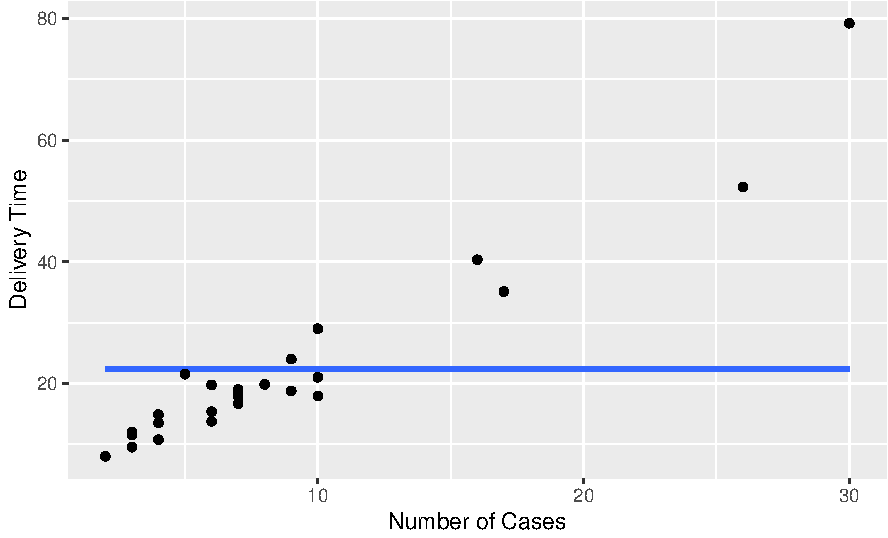
\includegraphics[width=0.7\linewidth]{regression-analysis_files/figure-latex/ybarpred-1} 

}

\caption{Regression without predictor}\label{fig:ybarpred}
\end{figure}

See Figure \ref{fig:ybarpred}. The line represents the closest line when we use only intercept term for the regression model. In other words, \emph{if we use no information for the response}, i.e.~no predictor variables, we will get just average of the response variable. Consider

\[Y_i = \beta_0 + \epsilon_i\]

Then we can get only one normal equation

\[\sum (Y_i - \hat\beta_0) = 0\]

Hence,

\[\hat\beta_0 = \frac{1}{n} \sum_{i = 1}^n Y_i \equiv \overline{Y}\]

From this fact, \(SST\) implies \textbf{total variance}.

\hypertarget{regression-sum-of-squares}{%
\subsection{Regression sum of squares}\label{regression-sum-of-squares}}

\BeginKnitrBlock{definition}[Regression Sum of Squares]
\protect\hypertarget{def:ssr}{}{\label{def:ssr} \iffalse (Regression Sum of Squares) \fi{} }\[SSR := \sum_{i = 1}^n (\hat{Y_i} - \overline{Y})^2\]
\EndKnitrBlock{definition}

This \(SSR\) compares \(\hat{Y_i}\) versus \(\overline{Y}\), computing the sum of squares for difference between predicted values from \emph{regression model} and \emph{model not using predictors}.

\hypertarget{residual-sum-of-squares}{%
\subsection{Residual sum of squares}\label{residual-sum-of-squares}}

Now consider the \emph{residual sum of squares} \(SSE\) in the definition \ref{def:sse}. As mentioned, this is related to the \emph{prediction errors}, which the regression model could not explain the data.

\hypertarget{decompsst}{%
\subsection{Decomposition of total sum of squares}\label{decompsst}}

\(SST\) can be decomposed by construction of sum of squares.

\BeginKnitrBlock{proposition}[Decomposition of SST]
\protect\hypertarget{prp:decom}{}{\label{prp:decom} \iffalse (Decomposition of SST) \fi{} }\[SST = SSR + SSE\]

where \(SST = \sum (Y_i - \overline{Y})^2\), \(SSR = \sum (\hat{Y_i} - \overline{Y})^2\), and \(SSE = \sum (Y_i - \hat{Y_i})\)
\EndKnitrBlock{proposition}

\BeginKnitrBlock{proof}
\iffalse{} {Proof. } \fi{}From the Example \ref{exm:usingnormal},

\begin{equation*}
  \begin{split}
    \sum_{i = 1}^n (Y_i - \overline{Y})^2 & = \sum_{i = 1}^n (Y_i - \hat{Y_i} + \hat{Y_i} - \overline{Y})^2 \\
    & = \sum_{i = 1}^n (Y_i - \hat{Y_i})^2 + 2 \sum_{i = 1}^n (Y_i - \hat{Y_i})(\hat{Y_i} - \overline{Y}) + \sum_{i = 1}^n (\hat{Y_i} - \overline{Y})^2 \\
    & = \sum_{i = 1}^n (Y_i - \hat{Y_i})^2 + \sum_{i = 1}^n (\hat{Y_i} - \overline{Y})^2 \qquad \because \sum (Y_i - \hat{Y_i}) = 0 \: \text{and} \: \sum (Y_i - \hat{Y_i})\hat{Y_i} = 0
  \end{split}
\end{equation*}
\EndKnitrBlock{proof}

This represents each \(SSR\) and \(SSE\) divides total variability as following.

\[\overset{SST}{\text{total variability}} = \overset{SSR}{\text{explained by regression}} + \overset{SSE}{\text{left unexplained by regression}}\]

Denote that the total variability \(SST\) is \emph{constant given data set}. If our model is good, \(SSR\) grows and \(SSE\) flattens. Thus the larger \(SSR\) is, the better. The lower \(SSE\) is, the better.

\hypertarget{coefficient-of-determination}{%
\subsection{Coefficient of determination}\label{coefficient-of-determination}}

We have discussed in the previous section \ref{decompsst} that \(SSR\) and \(SSE\) splits the total variability into \emph{explained part and not-explained part by our regression model}. Our first interest is whether the model works well for the data well, so we can think about the \emph{proportion of explained part to the total variance}. The following measure \(R^2\) computes this kind of value.

\BeginKnitrBlock{definition}[Coefficient of Determination]
\protect\hypertarget{def:rsq}{}{\label{def:rsq} \iffalse (Coefficient of Determination) \fi{} }\[R^2 := \frac{SSR}{SST} = 1 - \frac{1 - SSE}{SST}\]
\EndKnitrBlock{definition}

By construction,

\[0 \le R^2 \le 1\]

As \(R^2\) goes to \(0\), the model goes wrong. As \(R^2\) is close to \(1\), large proportion of variability has been explained. So we prefer large values rather than small.

\BeginKnitrBlock{proposition}
\protect\hypertarget{prp:rsqlin}{}{\label{prp:rsqlin} }\(R^2\) shows the strength of linear relation between two variables \(x\) and \(Y\) in the simple linear regression.

\[R^2 = \hat\rho_{XY}\]

where \(\hat\rho_{XY} := \frac{\sum (X_i - \overline{X})(Y_i - \overline{Y})}{\sqrt{\sum (X_i - \overline{X})^2} \sqrt{\sum (Y_i - \overline{Y})^2}}\) is the sample correlation coefficients
\EndKnitrBlock{proposition}

\BeginKnitrBlock{proof}
\iffalse{} {Proof. } \fi{}Note that \(\hat{Y_i} - \overline{Y} = \hat\beta_1 (x_i - \overline{x}) = \frac{S_{XY}}{S_{XX}} (x_i - \overline{x})\). Then

\begin{equation*}
  \begin{split}
    \sum (\hat{Y_i} - \overline{Y})^2 & = \frac{S_{XY}^2}{S_{XX}^2} \sum (x_i - \overline{x})^2 \\
    & = \frac{S_{XY}^2}{S_{XX}}
  \end{split}
\end{equation*}

It follows that

\begin{equation*}
  \begin{split}
    R^2 & = \frac{\sum (\hat{Y_i} - \overline{Y})^2}{\sum (Y_i - \overline{Y})^2} \\
    & = \frac{S_{XY}^2}{S_{XX}S_{YY}} \\
    & =: \hat\rho_{XY}^2
  \end{split}
\end{equation*}
\EndKnitrBlock{proof}

In this relation, we can know that \(R^2\) statistic performs as a measure of the linear relationship in the simple linear regression setting.

\hypertarget{matnot}{%
\section{Geometric Interpretations}\label{matnot}}

\hypertarget{fundamental-subspaces}{%
\subsection{Fundamental subspaces}\label{fundamental-subspaces}}

These linear algebra concepts might be more useful for \emph{multiple linear regression}, but let's briefly recap \citep{Leon:2014aa}.

\BeginKnitrBlock{definition}[Fundamental Subspaces]
\protect\hypertarget{def:subspace}{}{\label{def:subspace} \iffalse (Fundamental Subspaces) \fi{} }Let \(X \in \mathbb{R}^{n \times (p + 1)}\).

Then the Null space is defined by

\[N(X) := \{ \mathbf{b} \in \mathbb{R}^n \mid X\mathbf{b} = \mathbf{0} \}\]

The Row space is defined by

\[Row(X) := sp(\{\mathbf{r}_1, \ldots, \mathbf{r}_{p + 1} \}) \quad \text{where} \: X^T = [\mathbf{r}_1^T, \ldots, \mathbf{r}_{n}^T]\]

The Column space is defined by

\[Col(X) := sp(\{\mathbf{c}_1, \ldots, \mathbf{c}_{n} \}) \quad \text{where} \: X = [\mathbf{c}_1, \ldots, \mathbf{c}_{p + 1}]\]

The Range of \(X\) is defined by

\[R(X) := \{ \mathbf{y} \in \mathbb{R}^n \mid \mathbf{y} = X\mathbf{b} \quad \text{for some} \: \mathbf{b} \in \mathbb{R}^{p + 1} \}\]
\EndKnitrBlock{definition}

These spaces have some constructional relationship.

\BeginKnitrBlock{theorem}[Fundamental Subspaces Theorem]
\protect\hypertarget{thm:fundsub}{}{\label{thm:fundsub} \iffalse (Fundamental Subspaces Theorem) \fi{} }Let \(X \in \mathbb{R}^{n \times (p + 1)}\). Then

\[N(X) = R(X^T)^{\perp} = Col(X^T)^{\perp} = Row(X)^{\perp}\]

Transposed matrix also satisfy this.

\[N(X^T) = R(X)^{\perp} = Col(X)^{\perp}\]
\EndKnitrBlock{theorem}

\BeginKnitrBlock{proof}
\iffalse{} {Proof. } \fi{}Let \(\mathbf{a} \in N(X)\). Then \(X\mathbf{a} = \mathbf{0}\).

Let \(\mathbf{y} \in R(X^T)\). Then \(X^T \mathbf{b} = \mathbf{y}\) for some \(\mathbf{b} \in \mathbb{R}^{p + 1}\).

Choose \(\mathbf{b} \in \mathbb{R}^{p + 1}\) such that \(X^T \mathbf{b} = \mathbf{y}\). Then

\begin{equation*}
  \begin{split}
    \mathbf{0} & = X\mathbf{a} \\
    & = \mathbf{b}^T X\mathbf{a} \\
    & = \mathbf{y}^T \mathbf{a}
  \end{split}
\end{equation*}

Hence,

\[N(X) \perp R(X^T)\]

Since

\[X^T \mathbf{b} = \mathbf{c}_1 \mathbf{b} + \cdots + \mathbf{c}_{p + 1} \mathbf{b}\]

it is trivial that \(R(X) = Col(X)\) and \(R(X^T) = Col(X^T)\).

If \(\mathbf{a} \in N(X)\), then

\[
X\mathbf{a} = \begin{bmatrix}
  \mathbf{r}_1 \\
  \mathbf{r}_2 \\
  \cdots \\
  \mathbf{r}_n
\end{bmatrix} \begin{bmatrix}
  a_1 \\
  \cdots \\
  a_{p + 1}
\end{bmatrix} = \begin{bmatrix}
  0 \\
  0 \\
  \cdots \\
  0
\end{bmatrix}
\]

Thus,

\[\forall i :  \mathbf{a}^T \mathbf{r}_i = 0\]

and so

\[N(X) \subseteq Row(X)^{\perp}\]

Conversely, if \(\mathbf{a} \in Row(X)^{\perp}\), then \(\forall i : \mathbf{a}^T \mathbf{r}_i = 0\). This implies that \(X\mathbf{a} = \mathbf{0}\). Thus,

\[Row(X)^{\perp} \subseteq N(X)\]

and so

\[N(X) = Row(X)^{\perp}\]
\EndKnitrBlock{proof}

\(N(X^T) = R(X)^{\perp}\) part in Theorem \ref{thm:fundsub} will give the geometric insight to \emph{least squares solution}.

\BeginKnitrBlock{theorem}
\protect\hypertarget{thm:perpbasis}{}{\label{thm:perpbasis} }Let \(S\) be a subspace of \(\mathbb{R}^n\). Then

\[dim S + dim S^{\perp} = n\]

If \(\{ \mathbf{x}_1, \ldots, \mathbf{x}_r \}\) is a basis for \(S\) and \(\{ \mathbf{x}_{r + 1}, \ldots, \mathbf{x}_n \}\) is a basis for \(S^{\perp}\), then \(\{ \mathbf{x}_1, \ldots, \mathbf{x}_r, \mathbf{x}_{r + 1}, \ldots, \mathbf{x}_n \}\) is a basis for \(\mathbb{R}^n\).
\EndKnitrBlock{theorem}

\BeginKnitrBlock{theorem}
\protect\hypertarget{thm:dsum}{}{\label{thm:dsum} }Let \(S\) be a subspace of \(\mathbb{R}^n\). Then

\[\mathbb{R}^n = S \oplus S^{\perp}\]
\EndKnitrBlock{theorem}

\hypertarget{simple-linear-regression}{%
\subsection{Simple linear regression}\label{simple-linear-regression}}

\BeginKnitrBlock{theorem}
\protect\hypertarget{thm:projection}{}{\label{thm:projection} }Let \(S\) be a subspace of \(\mathbb{R}^n\). For each \(\mathbf{y} \in \mathbf{R}^n\), there exists a unique \(\mathbf{p} \in S\) that is closest to \(\mathbf{y}\), i.e.

\[\Vert \mathbf{y} - \mathbf{p}  \Vert > \Vert \mathbf{y} - \mathbf{\hat{y}} \Vert\]

for any \(\mathbf{p} \neq \mathbf{\hat{y}}\). Furthermore, a given vector \(\mathbf{p} \in S\) will be the closest to a given vector \(\mathbf{y} \in \mathbb{R}^n\) if and only if

\[\mathbf{y} - \mathbf{\hat{y}} \in S^{\perp}\]
\EndKnitrBlock{theorem}

Least square estimator \((\hat\beta_0, \hat\beta_1)^T\) minimizes

\begin{equation}
  \sum_{i = 1}^n (Y_i - \beta_0 - \beta_1 x_i)^2 = \Vert \mathbf{Y} - (\beta_0 \mathbf{1} + \beta_1 \mathbf{x}) \Vert^2
  \label{eq:qmatrix}
\end{equation}

with respect to \((\hat\beta_0, \hat\beta_1)^T \in \mathbb{R}^2\) (where \(\mathbf{1} := (1, 1)^T\)). Recall that the normal equation gives

\[\sum_{i = 1}^n(Y_i - \hat\beta_0 - \hat\beta_1 x_i) = \Big( \mathbf{Y} - (\hat\beta_0 \mathbf{1} + \hat\beta_1 \mathbf{x}) \Big)^T \mathbf{1} = 0\]

and

\[\sum_{i = 1}^n (Y_i - \hat\beta_0 - \hat\beta_1 x_i)x_i = \Big( \mathbf{Y} - (\hat\beta_0 \mathbf{1} + \hat\beta_1 \mathbf{x}) \Big)^T \mathbf{x} = 0\]

These two relation give

\[\mathbf{Y} - (\hat\beta_0 \mathbf{1} + \hat\beta_1 \mathbf{x}) \perp sp(\{ \mathbf{1}, \mathbf{x} \})^{\perp}\]

i.e.~\(\mathbf{\hat{Y}} = \hat\beta_0 \mathbf{1} + \hat\beta_1 \mathbf{x}\) is the projection of \(\mathbf{Y}\).

Theorem \ref{thm:projection} can give the same result.

\[\hat\beta_0 \mathbf{1} + \hat\beta_1 \mathbf{x} \in R([\mathbf{1}, \mathbf{x}])^{\perp} = sp(\{ \mathbf{1}, \mathbf{x} \})^{\perp}\]

\begin{figure}[H]

{\centering 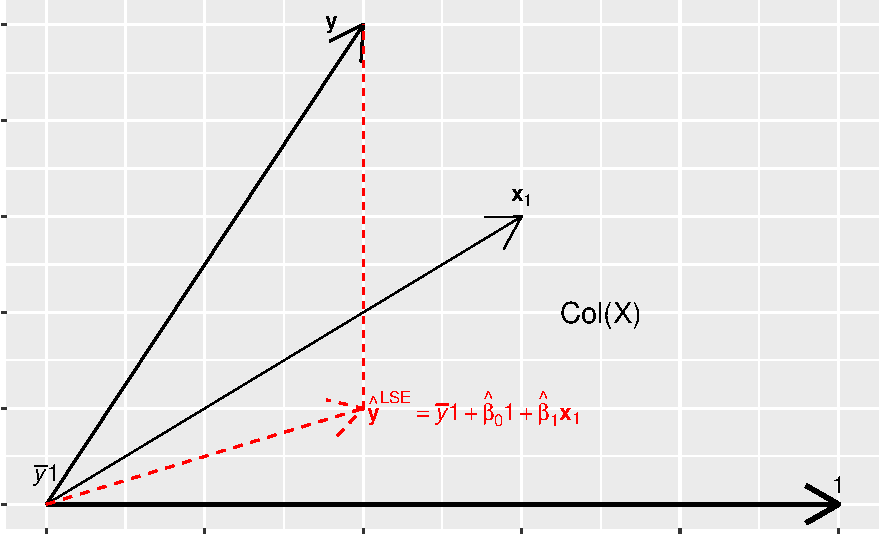
\includegraphics[width=0.7\linewidth]{regression-analysis_files/figure-latex/simpledraw-1} 

}

\caption{Geometric Illustration of Simple Linear Regression}\label{fig:simpledraw}
\end{figure}

We can see the details from Figure \ref{fig:simpledraw}. In fact, decomposition of \(SST\) and \(R^2\) are also in here.

\begin{figure}[H]

{\centering 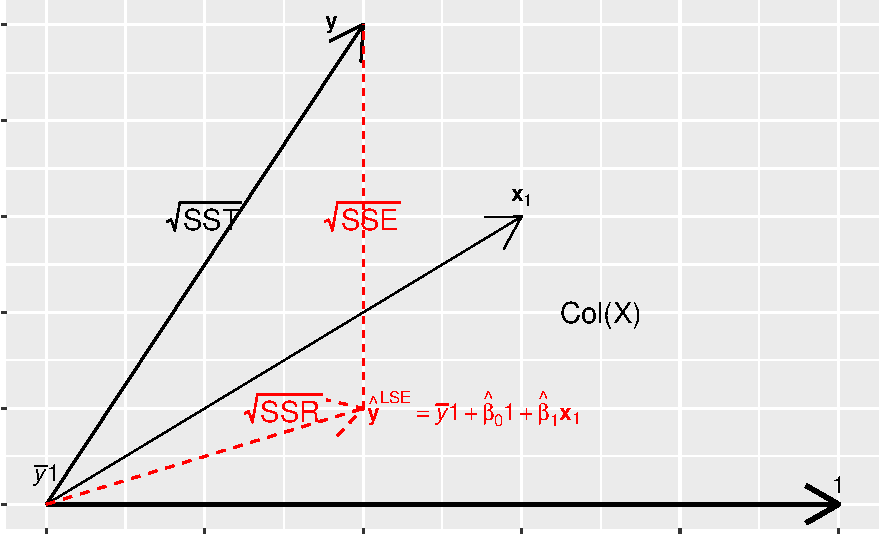
\includegraphics[width=0.7\linewidth]{regression-analysis_files/figure-latex/simpledraw2-1} 

}

\caption{Geometric Illustration of Decomposing SST}\label{fig:simpledraw2}
\end{figure}

See Figure \ref{fig:simpledraw2}.

\[
\begin{cases}
  SST = \lVert \mathbf{Y} - \overline{Y} \mathbf{1} \rVert^2 \\
  SSR = \lVert \mathbf{\hat{Y}} - \overline{Y} \mathbf{1} \rVert^2 \\
  SSE = \lVert \mathbf{Y} - \mathbf{\hat{Y}} \rVert^2
\end{cases}
\]

Pythagorean law implies that

\[SST = SSR + SSE\]

Also,

\begin{equation}
  R^2 = \frac{SSR}{SST} = cos^2\theta = \hat\rho_{XY}^2
  \label{eq:rsqcos}
\end{equation}

\hypertarget{solproj}{%
\subsection{Projection mapping}\label{solproj}}

Look again Figure \ref{fig:simpledraw}. Let \(X \equiv [\mathbf{1}, \mathbf{x}] \in \mathbb{R}^{n \times 2}\) and let \(\boldsymbol\beta \equiv (\beta_0, \beta_1)^T\). By the fundamental subspaces theorem \ref{thm:fundsub},

\[\mathbf{Y} - X\boldsymbol{\hat\beta} \in Col(X)^{\perp} = N(X^T)\]

Thus,

\begin{equation}
  X^T(\mathbf{Y} - X\boldsymbol{\hat\beta}) = \mathbf{0}
  \label{eq:projeq}
\end{equation}

This is the another representation of normal equation. Then we now have

\begin{equation*}
  \begin{split}
    & X^T\mathbf{Y} - X^TX\boldsymbol{\hat\beta} = \mathbf{0} \\
    & \Leftrightarrow X^T\mathbf{Y} = X^TX\boldsymbol{\hat\beta}
  \end{split}
\end{equation*}

If \(X^TX\) is nonsingular,

\[\boldsymbol{\hat\beta} = (X^TX)^{-1}X^T \mathbf{Y}\]

It follows that

\[\mathbf{\hat{Y}} = X\boldsymbol{\hat\beta} = X(X^TX)^{-1}X^T \mathbf{Y}\]

Combining this equation and our figure, we can know that \(X(X^TX)^{-1}X^T\) projects \(\mathbf{Y}\) from \(\mathbb{R}^n\) onto \(Col(X) = R(X)\). This is called projection operator/mapping.

\BeginKnitrBlock{definition}[Projection matrix]
\protect\hypertarget{def:projop}{}{\label{def:projop} \iffalse (Projection matrix) \fi{} }Projection operator or mapping from \(\mathbb{R}^n\) to \(W\) is written by

\[\Pi(\cdot \mid W) := X(X^TX)^{-1}X^T\]

It can also be called \textbf{\textit{Hat matrix}} and written as \(H\).
\EndKnitrBlock{definition}

As mentioned, \(X^TX\) should be invertible to get the LSE solution.

\BeginKnitrBlock{theorem}
\protect\hypertarget{thm:fullrank}{}{\label{thm:fullrank} }Let \(\mathbf{Y} = X\boldsymbol\beta\) inconsistent and let \(X \in \mathbb{R}^{n \times (p + 1)}\) with \(n > p + 1\).

If \(rank(X) = p + 1\), i.e.~full rank, then \(X^T X\) is invertible.
\EndKnitrBlock{theorem}

\BeginKnitrBlock{proof}
\iffalse{} {Proof. } \fi{}Suppose that \((X^TX)\mathbf{b} = \mathbf{0}\). Then

\[X^T (X\mathbf{b}) = \mathbf{0}\]

By the fundamental subspaces theorem \ref{thm:fundsub},

\[X\mathbf{b} \in N(X^T) = Col(X)^{\perp}\]

By construction,

\[X\mathbf{b} \in Col(X) = N(X^T)^{\perp}\]

Then

\[X\mathbf{b} \in N(X^T) \cap N(X^T)^{\perp} = \{ \mathbf{0} \}\]

It follows that

\[X\mathbf{b} = \mathbf{0}\]

If \(rank(X) = \min(n, p + 1)\), then the linear equation system has trivial solution \(\mathbf{b} = \mathbf{0}\) and so does \(X^T (X\mathbf{b}) = \mathbf{0}\). Hence, \(X^T X\) is invertible.
\EndKnitrBlock{proof}

Using projection matrix \(\Pi_W\), we can re-express each sum of squares. Recall that when we only use \(y_i\) for regression fitting, the result becomes its average. It is because \(\mathbf{Y}\) vector has been projected onto \(sp(\{ \mathbf{1} \})\) line.

\BeginKnitrBlock{remark}
\iffalse{} {Remark. } \fi{}\[\overline{Y}\mathbf{1} = \mathbf{1}(\mathbf{1}^T\mathbf{1})^{-1}\mathbf{1}^T\mathbf{Y} = \Pi_{\mathbf{1}}\mathbf{Y}\]

\[\mathbf{\hat{Y}} = X(X^TX)^{-1}X^T \mathbf{Y} = \Pi_X \mathbf{Y}\]
\EndKnitrBlock{remark}

Intuitively, every projection matrix is idempotent and symmetric. Once projected, the result is same when projecting it again.

\BeginKnitrBlock{corollary}[Sum of squares]
\protect\hypertarget{cor:projss}{}{\label{cor:projss} \iffalse (Sum of squares) \fi{} }\(\Pi_{\mathbf{1}}\) and \(\Pi_X\) can express each \(SS\) as following.

\begin{enumerate}[label=(\roman*)]
  \item $$SST = \mathbf{Y}^T (I - \Pi_{\mathbf{1}}) \mathbf{Y}$$
  \item $$SSR = \mathbf{Y}^T (\Pi_X - \Pi_{\mathbf{1}}) \mathbf{Y}$$
  \item $$SSE = \mathbf{Y}^T (I - \Pi_X) \mathbf{Y}$$
\end{enumerate}
\EndKnitrBlock{corollary}

\hypertarget{simpledist}{%
\section{Distributions}\label{simpledist}}

\hypertarget{mean-response-and-response}{%
\subsection{Mean response and response}\label{mean-response-and-response}}

We have already look at predicting each mean response and response from equation \eqref{eq:meanres} and \eqref{eq:indpred}.

\BeginKnitrBlock{theorem}[Estimation of the mean response]
\protect\hypertarget{thm:mux}{}{\label{thm:mux} \iffalse (Estimation of the mean response) \fi{} }\[\hat\mu_x \equiv \widehat{E(Y \mid x)} = \hat\beta_0 + \hat\beta_1 x\]
\EndKnitrBlock{theorem}

\BeginKnitrBlock{theorem}[(out of sample) Prediction of a response]
\protect\hypertarget{thm:yhatx}{}{\label{thm:yhatx} \iffalse ((out of sample) Prediction of a response) \fi{} }\[\hat{Y_x}  = \hat\beta_0 + \hat\beta_1 x\]
\EndKnitrBlock{theorem}

Recall that predicting \ref{thm:mux} targets at

\[\mu_x \equiv E(Y \mid x) = \beta_0 + \beta_1 x\]

which have been assumed to be true model. On the other hand, predicting \ref{thm:yhatx} targets at

\[Y = \beta_0 + \beta_1 + \epsilon_x\]

The linearity is not true in reality. So the errors caused by modeling linear model are included in \(\epsilon_x\). This error term makes difference between properties of \ref{thm:mux} and \ref{thm:yhatx}.

To derive their distribution and see the difference, we additionaly assume Normality, i.e.

\[\epsilon_i \stackrel{iid}{\sim} N(0, \sigma^2)\]

\hypertarget{simplebdist}{%
\subsection{Regression coefficients}\label{simplebdist}}

Under Normality, we have

\[Y_i \stackrel{indep}{\sim} N(\beta_0 + \beta_1 x_i, \sigma^2)\]

Then

\[
\mathbf{Y} = \begin{bmatrix}
  Y_1 \\
  Y_2 \\
  \vdots \\
  Y_n
\end{bmatrix} \sim MVN_n\Bigg( \boldsymbol\mu \equiv \begin{bmatrix}
  \beta_0 + \beta_1 x_1 \\
  \beta_0 + \beta_1 x_2 \\
  \vdots \\
  \beta_0 + \beta_1 x_n
\end{bmatrix}, \Sigma \equiv \sigma^2 I = \begin{bmatrix}
  \sigma^2 & 0 & \cdots & 0 \\
  0 & \sigma^2 & \cdots & 0 \\
  \vdots & \vdots & \vdots & \vdots \\
  0 & 0 & 0 & \sigma^2
\end{bmatrix} \Bigg)
\]

Write \(\boldsymbol{\hat\beta} = (\hat\beta_0, \hat\beta_1)^T\). From Lemma \ref{lem:linbet},

\[\hat\beta_0 = \mathbf{a}^T\mathbf{Y}\]

where \(\mathbf{a} = (a_1, \ldots, a_n)^T \in \mathbb{R}^n\) with \(a_i = \bigg( \frac{1}{n} - \frac{(x_i - \overline{x})\overline{x}}{S_{XX}} \bigg)\)

and

\[\hat\beta_1 = \mathbf{b}^T\mathbf{Y}\]

where \(\mathbf{b} = (b_1, \ldots, b_n)^T \in \mathbb{R}^n\) with \(b_i = \frac{(x_i - \overline{x})}{S_{XX}}\).

Let

\[
A = \begin{bmatrix}
  \mathbf{a}^T \\ \hline
  \mathbf{b}^T
\end{bmatrix} \in \mathbb{R}^{2 \times n}
\]

Then

\[
\boldsymbol{\hat\beta} = A\mathbf{Y}
\]

Linearity of the multivariate normal distribution, Proposition \ref{prp:ue} and \ref{prp:vb} imply that

\begin{equation}
  \boldsymbol{\hat\beta} = \begin{bmatrix}
    \hat\beta_0 \\ \hline
    \hat\beta_1
  \end{bmatrix} \sim MVN \bigg( A\boldsymbol\mu = \begin{bmatrix}
    \beta_0 \\ \hline
    \beta_1
  \end{bmatrix},
  A\Sigma A^T = \sigma^2 AA^T = \begin{bmatrix}
    \bigg( \frac{1}{n} + \frac{\overline{x}^2}{S_{XX}} \bigg)\sigma^2 & - \frac{\overline{x}}{S_{XX}}\sigma^2 \\ \hline
    - \frac{\overline{x}}{S_{XX}}\sigma^2 & \frac{\sigma^2}{S_{XX}}
  \end{bmatrix} \bigg)
  \label{eq:b01mvn}
\end{equation}

Since the joint random vector follows multivariate normal distribution, each \emph{partitioned subset follow normal}. For this theorem, see \citet{Johnson:2013aa}. Hence, we finally get the following result.

\BeginKnitrBlock{theorem}[Distributions of regression coefficients]
\protect\hypertarget{thm:b01dist}{}{\label{thm:b01dist} \iffalse (Distributions of regression coefficients) \fi{} }Each regression coefficient follows Normal distribution.

\[\hat\beta_0 \sim N \bigg( \beta_0, \bigg( \frac{1}{n} + \frac{\overline{x}^2}{S_{XX}} \bigg)\sigma^2 \bigg)\]

\[\hat\beta_1 \sim N \bigg( \beta_1, \frac{\sigma^2}{S_{XX}} \bigg)\]
\EndKnitrBlock{theorem}

\hypertarget{mean-response}{%
\subsection{Mean response}\label{mean-response}}

In simple linear regression setting, we assume \(\mu_x = E(Y \mid x) = \beta_0 + \beta_1 x\) is true.

\begin{Shaded}
\begin{Highlighting}[]
\NormalTok{delv }\OperatorTok\StringTok{ }
\StringTok{  }\KeywordTok{ggplot}\NormalTok{(}\KeywordTok{aes}\NormalTok{(}\DataTypeTok{x =}\NormalTok{ x, }\DataTypeTok{y =}\NormalTok{ y)) }\OperatorTok{+}
\StringTok{  }\KeywordTok{geom_smooth}\NormalTok{(}\DataTypeTok{method =} \StringTok{"lm"}\NormalTok{) }\OperatorTok{+}
\StringTok{  }\KeywordTok{geom_point}\NormalTok{(}\DataTypeTok{alpha =} \FloatTok{.7}\NormalTok{) }\OperatorTok{+}
\StringTok{  }\KeywordTok{labs}\NormalTok{(}
    \DataTypeTok{x =} \StringTok{"Number of Cases"}\NormalTok{,}
    \DataTypeTok{y =} \StringTok{"Delivery Time"}
\NormalTok{  )}
\end{Highlighting}
\end{Shaded}

\begin{figure}[H]

{\centering 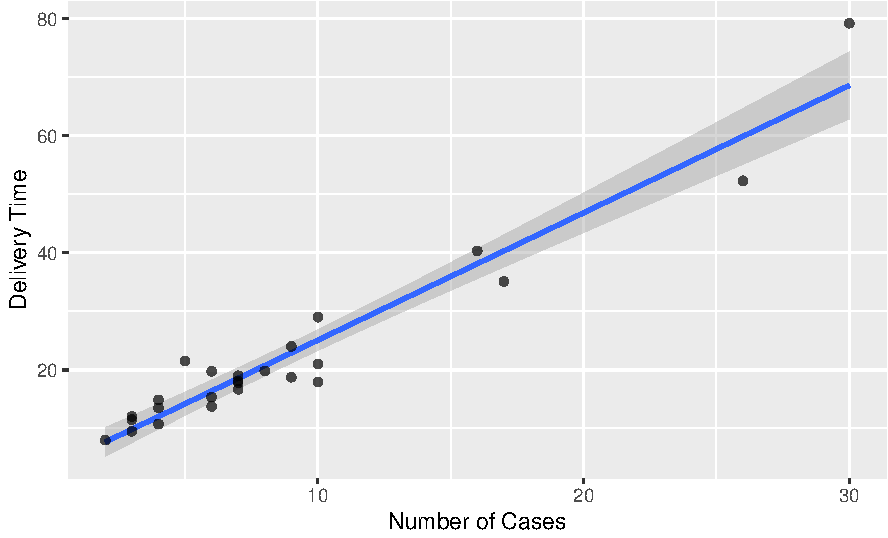
\includegraphics[width=0.7\linewidth]{regression-analysis_files/figure-latex/smoothline-1} 

}

\caption{Mean response and its standard deviation}\label{fig:smoothline}
\end{figure}

For example, in the Figure \ref{fig:smoothline}, the blue line indicates \(E(Y \mid X = x)\) for each point \(x\). Without fitting using \texttt{lm()}, \texttt{geom\_smooth(method\ =\ "lm")} let us visualize the fitted line. Since the default method is not the linear regression, the \texttt{method} option should be specified.

\begin{Shaded}
\begin{Highlighting}[]
\NormalTok{delv }\OperatorTok\StringTok{ }
\StringTok{  }\KeywordTok{mutate}\NormalTok{(}\DataTypeTok{eyx =} \KeywordTok{predict}\NormalTok{(delv_fit, }\DataTypeTok{newdata =} \KeywordTok{data.frame}\NormalTok{(}\DataTypeTok{x =}\NormalTok{ x)))}
\CommentTok{#> # A tibble: 25 x 3}
\CommentTok{#>        y     x   eyx}
\CommentTok{#>    <dbl> <dbl> <dbl>}
\CommentTok{#>  1  16.7     7 18.6 }
\CommentTok{#>  2  11.5     3  9.85}
\CommentTok{#>  3  12.0     3  9.85}
\CommentTok{#>  4  14.9     4 12.0 }
\CommentTok{#>  5  13.8     6 16.4 }
\CommentTok{#>  6  18.1     7 18.6 }
\CommentTok{#>  7   8       2  7.67}
\CommentTok{#>  8  17.8     7 18.6 }
\CommentTok{#>  9  79.2    30 68.6 }
\CommentTok{#> 10  21.5     5 14.2 }
\CommentTok{#> # ... with 15 more rows}
\end{Highlighting}
\end{Shaded}

We have already seen in section \ref{simplebdist} that the estimators \(\hat\beta_0\) and \(\hat\beta_1\) are random variables. So \(\hat\mu_x\) is. In fact, the ribbon of the line in Figure \ref{fig:smoothline} represents upper and lower confidence limits on mean response. In the later section, we get to know that it is \(+ t(n - 2)\widehat{SE}(\hat\mu_x)\) and \(- t(n - 2) \widehat{SE}(\hat\mu_x)\). It can be drawn by default with the option of the \texttt{geom\_smooth(se\ =\ TRUE)}.

\BeginKnitrBlock{theorem}[Distribution of mean response estimator]
\protect\hypertarget{thm:mrdist}{}{\label{thm:mrdist} \iffalse (Distribution of mean response estimator) \fi{} }\(\hat\mu_x\) is also Normally distributed.

\[\hat\mu_x \sim N\bigg( \mu_x, \sigma^2\bigg( \frac{1}{n} + \frac{(x - \overline{x})^2}{S_{XX}} \bigg) \bigg)\]
\EndKnitrBlock{theorem}

\BeginKnitrBlock{proof}
\iffalse{} {Proof. } \fi{}Since \(\hat\mu_x = \hat\beta_0 + \hat\beta_1 x\) is the linear combination of \((\hat\beta_0, \hat\beta_1)^T\),

\[\hat\mu_x \sim N\Big(E(\hat\mu_x), Var(\hat\mu_x)\Big)\]

From Theorem \ref{thm:b01dist},

\[E(\hat\mu_x) = E(\hat\beta_0) + E(\hat\beta_1)x = \beta_0 + \beta_1x \equiv \mu_x\]

and from Proposition \ref{prp:vb}

\begin{equation*}
  \begin{split}
    Var(\hat\mu_x) & = Var(\hat\beta_0 + \hat\beta_1 x) \\
    & = Var(\hat\beta_0) + x^2Var(\hat\beta_1) + 2xCov(\hat\beta_0, \hat\beta_1) \\
    & = \bigg( \frac{1}{n} + \frac{\overline{x}^2}{S_{XX}} \bigg)\sigma^2 + \frac{x^2\sigma^2}{S_{XX}} - \frac{2\overline{x}x\sigma^2}{S_{XX}} \\
    & = \sigma^2\bigg(\frac{1}{n} + \frac{(x - \overline{x})^2}{S_{XX}} \bigg)
  \end{split}
\end{equation*}
\EndKnitrBlock{proof}

\BeginKnitrBlock{corollary}
\protect\hypertarget{cor:mrdiff}{}{\label{cor:mrdiff} }\[\hat\mu_x - \mu_x \sim N\bigg( 0, \sigma^2\bigg( \frac{1}{n} + \frac{(x - \overline{x})^2}{S_{XX}} \bigg) \bigg)\]
\EndKnitrBlock{corollary}

Denote that in both Theorem \ref{thm:mrdist} and Corollary \ref{cor:mrdiff}, \(\sigma^2\) is parameter. So to use \(SE(\hat\mu_x) = \sqrt{Var(\hat\mu_x)}\) in practice we plug in its estimator, usually Equation \eqref{eq:siglse}.

\BeginKnitrBlock{corollary}[Standard error of mean response estimator]
\protect\hypertarget{cor:mrse}{}{\label{cor:mrse} \iffalse (Standard error of mean response estimator) \fi{} }\[\widehat{SE}(\hat\mu_x) = \hat\sigma \sqrt{\bigg( \frac{1}{n} + \frac{(x - \overline{x})^2}{S_{XX}} \bigg)}\]

where \(\hat\sigma^2 = MSE\)
\EndKnitrBlock{corollary}

\hypertarget{response}{%
\subsection{Response}\label{response}}

Our goal is to predict each response at each point, i.e.~\(Y_x = \beta_0 + \beta_1 x + \epsilon_x\). \(\epsilon_x \sim N(0, \sigma^2)\) is independent of the given data (\(\epsilon_1, \ldots, \epsilon_n\)). In this sense, this prediction is called \emph{out of sample prediction}. This setting makes difference between the \emph{residuals, which are correlated to the data}. See Proposition \ref{prp:resprop} for this. This is occurred because each \(\hat\beta_0\) and \(\hat\beta_1\) is linear combination of \(Y_1, \ldots, Y_n\), not \(Y_x\).

While \(Cov(Y_i, \hat{Y_i}) > 0, i = 1, \ldots, n\) (See Equation \eqref{eq:yyhat}), in case of out-of-sample \(Y_x\),

\[Cov(Y_x, \hat{Y_x}) = Cov(Y_x, \hat\beta_0 + \hat\beta_1 x) = 0\]

Hence, arithmetically, this \emph{out of sample prediction becomes to have larger standard error}.

\BeginKnitrBlock{proposition}[Joint distribution of coefficients and error term]
\protect\hypertarget{prp:bepsmvn}{}{\label{prp:bepsmvn} \iffalse (Joint distribution of coefficients and error term) \fi{} }\((\hat\beta_0, \hat\beta_1, \epsilon_x)^T\) is Normally distributed.
\EndKnitrBlock{proposition}

\BeginKnitrBlock{proof}
\iffalse{} {Proof. } \fi{}Want 1: \((\hat\beta_0, \hat\beta_1)^T \perp\!\!\!\perp \epsilon_x\)

We have

\begin{equation}
  \begin{split}
    Cov((\hat\beta_0, \hat\beta_1)^T, \epsilon_x) & = \Big[Cov(\hat\beta_i, \epsilon_x) \Big]_{2 \times 1} \\
    & = \bigg[Cov\bigg(\sum_{i = 1}^n k_i Y_i, \epsilon_x \bigg) \bigg]_{2 \times 1} \qquad k_i = \text{each linear coefficient for}\: \hat\beta_0, \hat\beta_1 \\
    & = \mathbf{0}
  \end{split}
  \label{eq:betaepsind}
\end{equation}

From Equation \eqref{eq:b01mvn},

\[(\hat\beta_0, \hat\beta_1)^T \sim MVN\]

and from assumption,

\[\epsilon_x \sim N(0, \sigma^2)\]

It follows from Equation \eqref{eq:betaepsind} that (\citet{Johnson:2013aa})

\[(\hat\beta_0, \hat\beta_1)^T \perp\!\!\!\perp \epsilon_x\]

Want 2: \((\hat\beta_0, \hat\beta_1, \epsilon_x)^T \sim MVN\)

From independency, we have (\citet{Johnson:2013aa})

\[
\begin{bmatrix}
  \hat\beta_0 \\
  \hat\beta_1 \\ \hline
  \epsilon_x
\end{bmatrix} \sim MVN_{2 + 1} \bigg( \begin{bmatrix}
  \beta_0 \\
  \beta_1 \\ \hline
  0
\end{bmatrix}, \left[
  \begin{array}{c|c}
    Cov(\boldsymbol{\hat\beta}) \in \mathbb{R}^{2 \times 2} & \mathbf{0} \in \mathbb{R}^2 \\ \hline
    \mathbf{0}^T \in \mathbb{R}^{2 \times 1} & \sigma^2
  \end{array}
\right] \bigg)
\]
\EndKnitrBlock{proof}

This proposition gives clue to distribution of prediction error.

\BeginKnitrBlock{theorem}[Distribution of out-of-sample prediction error]
\protect\hypertarget{thm:preddist}{}{\label{thm:preddist} \iffalse (Distribution of out-of-sample prediction error) \fi{} }Out of sample prediction error \(\hat{Y_x} - Y_x\) is Normally distributed

\[\hat{Y_x} - Y_x \sim N\bigg( 0, \sigma^2 \bigg( 1 + \frac{1}{n} + \frac{(x - \overline{x})^2}{S_{XX}} \bigg) \bigg)\]
\EndKnitrBlock{theorem}

\BeginKnitrBlock{proof}
\iffalse{} {Proof. } \fi{}Note that

\begin{equation*}
  \begin{split}
    \hat{Y_x} - Y_x & = (\hat\beta_0 + \hat\beta_1 x) - (\beta_0 + \beta_1 x + \epsilon_x) \\
    & = [1, x, -1] (\hat\beta_0, \hat\beta_1, \epsilon_x)^T - \beta_0 - \beta_1 x
  \end{split}
\end{equation*}

i.e.~\(\hat{Y_x} - Y_x\) is a linear combination of \((\hat\beta_0, \hat\beta_1, \epsilon_x)^T\). From prosition \ref{prp:bepsmvn},

\begin{equation}
  \begin{split}
    \hat{Y_x} - Y_x & \sim MVN \Bigg( [1, x, -1]\begin{bmatrix}
    \beta_0 \\
    \beta_1 \\
    0
    \end{bmatrix} - \beta_0 - \beta_1 x,
    [1, x, -1]
    \left[
      \begin{array}{c|c}
        Cov(\boldsymbol{\hat\beta}) \in \mathbb{R}^{2 \times 2} & \mathbf{0} \in \mathbb{R}^2 \\ \hline
        \mathbf{0}^T \in \mathbb{R}^{2 \times 1} & \sigma^2
      \end{array}
    \right]
    \begin{bmatrix}
      1 \\
      x \\
      -1
    \end{bmatrix}
     \Bigg) \\
    & \stackrel{d}{=} MVN \bigg( 0, \sigma^2\bigg( \frac{1}{n} + \frac{\overline{x}^2}{S_{XX}} - 2 \frac{\overline{x}x}{S_{XX}} + \frac{x^2}{S_{XX}} \bigg) + 1 \bigg) \\
    & \stackrel{d}{=} MVN \bigg( 0, \sigma^2\bigg( 1 + \frac{1}{n} + \frac{(x - \overline{x})^2}{S_{XX}} \bigg) \bigg)
  \end{split}
  \label{eq:prederrmvn}
\end{equation}
\EndKnitrBlock{proof}

Now we know the standard error of this out-of-sample prediction error.

\[SE(\hat{Y_x} - Y_x) = \sigma \sqrt{\bigg( 1 + \frac{1}{n} + \frac{(x - \overline{x})^2}{S_{XX}} \bigg)}\]

We can see this standard error is \emph{always larger than of mean response estimator} due to \(1\) in the bracket, i.e.~\(\sigma^2\). As mentioned, this is due to \(\epsilon\) term. When we estimate or predict the mean response the model have been assumed to be true. In this out-of-sample prediction setting, however, the model can be wrong. This assumption error is also included in \(\epsilon\) term and it is called \emph{irreducible error}, which cannot be reduced anymore.

\BeginKnitrBlock{remark}
\iffalse{} {Remark. } \fi{}\[SE(\hat\mu_x - \mu_x) < SE(\hat{Y_x} - Y_x)\]
\EndKnitrBlock{remark}

It might be more clear if we see the inequality in the above remark. We know the fact that \(\hat{Y_x}\) and \(Y_x\) are uncorrelated in this out-of-sample setting. \(Y_x\) is random variable, while \(\mu_x\) is constant. Then we can re-express the inequality as

\[SE(\hat\mu_x) < SE(\hat{Y_x}) + SE(Y_x)\]

Actually, both \(\hat\mu_x\) and \(\hat{Y_x}\) are estimated as \(\hat\beta_0 + \hat\beta_1 x\). Thus, \(SE(Y_x) = \sigma^2\) makes out-of-sample more noisy.

To use standard error practically, we use \(\hat\sigma^2\) as in corollary \ref{cor:mrse}.

\BeginKnitrBlock{corollary}[Standard error of out-of-sample prediction error]
\protect\hypertarget{cor:predse}{}{\label{cor:predse} \iffalse (Standard error of out-of-sample prediction error) \fi{} }\[\widehat{SE}(\hat{Y_x} - Y_x) = \hat\sigma \sqrt{\bigg( 1 + \frac{1}{n} + \frac{(x - \overline{x})^2}{S_{XX}} \bigg)}\]

where \(\hat\sigma^2 = MSE\)
\EndKnitrBlock{corollary}

\hypertarget{statistical-inference}{%
\section{Statistical Inference}\label{statistical-inference}}

Based on each distribution of estimator in section \ref{simpledist}, we can construct various inferece for each

\begin{itemize}
\tightlist
\item
  \(\beta_0\)
\item
  \(\beta_1\)
\item
  \(\mu_x\)
\item
  \(Y_x\)
\item
  \(\sigma^2\)
\end{itemize}

We can get the standard error for each coefficient through \texttt{summary()} function.

\begin{Shaded}
\begin{Highlighting}[]
\KeywordTok{summary}\NormalTok{(delv_fit)}
\CommentTok{#> }
\CommentTok{#> Call:}
\CommentTok{#> lm(formula = y ~ x, data = delv)}
\CommentTok{#> }
\CommentTok{#> Residuals:}
\CommentTok{#>    Min     1Q Median     3Q    Max }
\CommentTok{#> -7.581 -1.874 -0.349  2.181 10.634 }
\CommentTok{#> }
\CommentTok{#> Coefficients:}
\CommentTok{#>             Estimate Std. Error t value Pr(>|t|)    }
\CommentTok{#> (Intercept)    3.321      1.371    2.42    0.024 *  }
\CommentTok{#> x              2.176      0.124   17.55  8.2e-15 ***}
\CommentTok{#> ---}
\CommentTok{#> Signif. codes:  0 '***' 0.001 '**' 0.01 '*' 0.05 '.' 0.1 ' ' 1}
\CommentTok{#> }
\CommentTok{#> Residual standard error: 4.18 on 23 degrees of freedom}
\CommentTok{#> Multiple R-squared:  0.93,   Adjusted R-squared:  0.927 }
\CommentTok{#> F-statistic:  308 on 1 and 23 DF,  p-value: 8.22e-15}
\end{Highlighting}
\end{Shaded}

Or more state-or-art way, \texttt{broom:tidy()} function has a method for each model object to make tidy data: \texttt{tibble}.

\begin{Shaded}
\begin{Highlighting}[]
\NormalTok{broom}\OperatorTok{::}\KeywordTok{tidy}\NormalTok{(delv_fit)}
\CommentTok{#> # A tibble: 2 x 5}
\CommentTok{#>   term        estimate std.error statistic  p.value}
\CommentTok{#>   <chr>          <dbl>     <dbl>     <dbl>    <dbl>}
\CommentTok{#> 1 (Intercept)     3.32     1.37       2.42 2.37e- 2}
\CommentTok{#> 2 x               2.18     0.124     17.5  8.22e-15}
\end{Highlighting}
\end{Shaded}

\hypertarget{confidence-interval}{%
\subsection{Confidence interval}\label{confidence-interval}}

Consider standardization.

\[\frac{\hat\theta - \theta}{SE(\hat\theta)}\]

Each \(SE\) includes \(\sigma^2\) as we have already seen. First think about \textbf{known} \(\sigma^2\) setting. All three estimators follow Normal distribution, and \(SE\) is constant by our the setting. Then we can construct each confidence interval as

\[\hat\theta \pm z_{\frac{\alpha}{2}} SE(\hat\theta)\]

\begin{figure}[H]

{\centering 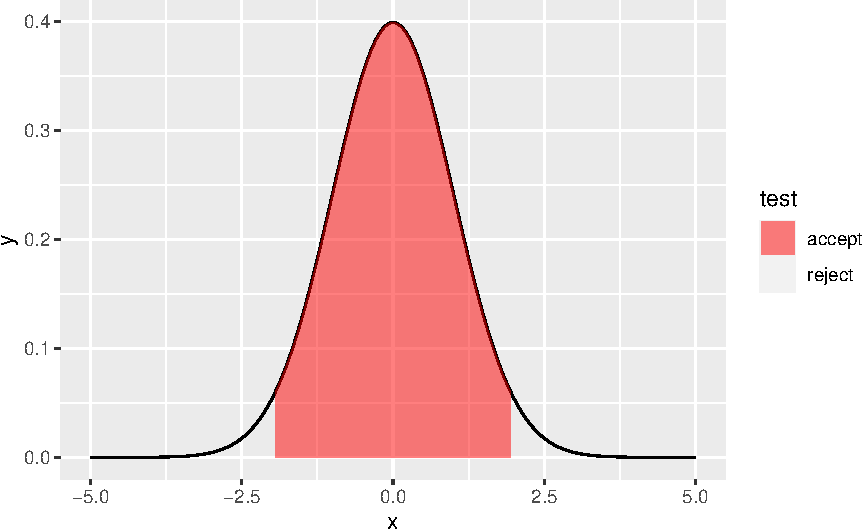
\includegraphics[width=0.7\linewidth]{regression-analysis_files/figure-latex/estci-1} 

}

\caption{Confidence Interval when $\sigma^2$ is known}\label{fig:estci}
\end{figure}

Now just plug in the results of section \ref{simpledist}. For each regression coefficient,

\BeginKnitrBlock{proposition}[Confidence intervals on $\beta$]
\protect\hypertarget{prp:betaci}{}{\label{prp:betaci} \iffalse (Confidence intervals on \(\beta\)) \fi{} }With known \(\sigma^2\), \((1 - \alpha)100 \%\) confidence intervals on \(\beta_0\) and \(\beta_1\) are given as

\[\beta_0 : \quad \hat\beta_0 \pm z_{\frac{\alpha}{2}} \sqrt{\bigg( \frac{1}{n} + \frac{\overline{x}^2}{S_{XX}} \bigg) \sigma^2}\]

\[\beta_1 : \quad \hat\beta_1 \pm z_{\frac{\alpha}{2}} \sqrt{\frac{\sigma^2}{S_{XX}}}\]
\EndKnitrBlock{proposition}

\BeginKnitrBlock{proposition}[Confidence interval on $\hat\mu_x$]
\protect\hypertarget{prp:mrci}{}{\label{prp:mrci} \iffalse (Confidence interval on \(\hat\mu_x\)) \fi{} }With known \(\sigma^2\), \((1 - \alpha)100 \%\) confidence interval on \(\hat\mu_x\) is given as

\[\mu_x : \quad \hat\mu_x \pm z_{\frac{\alpha}{2}} \sqrt{\sigma^2 \bigg( \frac{1}{n} + \frac{(x - \overline{x})^2}{S_{xx}} \bigg)}\]
\EndKnitrBlock{proposition}

In practice, however, we do not know \(\sigma^2\). In this case, we replace \(\sigma^2\) with \(\hat\sigma^2 = \frac{1}{n - 2}\sum\limits_{i = 1}^n (\hat{Y_i} - Y_i)^2 = MSE\). Then

\[\frac{\hat\theta - \theta}{\widehat{SE}} = \frac{\frac{\hat\theta - \theta}{\sqrt{Var = \sigma^2(\cdot)}}}{\sqrt{\frac{\frac{SSE}{\sigma^2}}{n - 2}\bigg( \cdot \bigg)}} =  \frac{\frac{\hat\theta - \theta}{\sqrt{Var = \sigma^2}} \sim N(0, 1)}{\sqrt{\frac{\frac{SSE}{\sigma^2} \sim \chi^2(n - 2)}{n - 2}}} \sim t(n - 2)\]

Thus, we need to replace \(z_{\frac{\alpha}{2}}\) with \(t_{\frac{\alpha}{2}}(n - 2)\).

\BeginKnitrBlock{proposition}[Confidence intervals on $\beta$ when unknown $\sigma^2$]
\protect\hypertarget{prp:betaci2}{}{\label{prp:betaci2} \iffalse (Confidence intervals on \(\beta\) when unknown \(\sigma^2\)) \fi{} }With unknown \(\sigma^2\), \((1 - \alpha)100 \%\) confidence intervals on \(\beta_0\) and \(\beta_1\) are given as

\[\beta_0 : \quad \hat\beta_0 \pm t_{\frac{\alpha}{2}}(n - 2) \sqrt{\bigg( \frac{1}{n} + \frac{\overline{x}^2}{S_{XX}} \bigg) \hat\sigma^2}\]

\[\beta_1 : \quad \hat\beta_1 \pm t_{\frac{\alpha}{2}}(n - 2) \sqrt{\frac{\hat\sigma^2}{S_{XX}}}\]

where \(\hat\sigma^2 = MSE\)
\EndKnitrBlock{proposition}

Here we can estimate the intervals. Basically, \texttt{confint()} function gives this interval.

\begin{Shaded}
\begin{Highlighting}[]
\KeywordTok{confint}\NormalTok{(delv_fit, }\DataTypeTok{level =} \FloatTok{.95}\NormalTok{)}
\CommentTok{#>             2.5 % 97.5 %}
\CommentTok{#> (Intercept) 0.484   6.16}
\CommentTok{#> x           1.920   2.43}
\end{Highlighting}
\end{Shaded}

\BeginKnitrBlock{proposition}[Confidence interval on $\hat\mu_x$ when unknown $\sigma^2$]
\protect\hypertarget{prp:mrci2}{}{\label{prp:mrci2} \iffalse (Confidence interval on \(\hat\mu_x\) when unknown \(\sigma^2\)) \fi{} }With unknown \(\sigma^2\), \((1 - \alpha)100 \%\) confidence interval on \(\hat\mu_x\) is given as

\[\mu_x : \quad \hat\mu_x \pm t_{\frac{\alpha}{2}}(n - 2) \sqrt{\hat\sigma^2 \bigg( \frac{1}{n} + \frac{(x - \overline{x})^2}{S_{xx}} \bigg)}\]

where \(\hat\sigma^2 = MSE\)
\EndKnitrBlock{proposition}

\texttt{predict()} provides options for this confidence interval. Specify \texttt{interval\ =\ "confidence"}. This argument has three option.

\begin{enumerate}
\def\labelenumi{\arabic{enumi}.}
\tightlist
\item
  \texttt{"none"}: just compute fitted value, by default.
\item
  \texttt{"confidence"}: confidence interval of mean response
\item
  \texttt{"prediction"}: prediction interval of out-of-sample prediction
\end{enumerate}

Default \texttt{level} is \texttt{0.95}.

\begin{Shaded}
\begin{Highlighting}[]
\KeywordTok{predict}\NormalTok{(delv_fit, }\DataTypeTok{interval =} \StringTok{"confidence"}\NormalTok{, }\DataTypeTok{level =} \FloatTok{.95}\NormalTok{) }\OperatorTok\StringTok{ }\KeywordTok{tbl_df}\NormalTok{()}
\CommentTok{#> # A tibble: 25 x 3}
\CommentTok{#>      fit   lwr   upr}
\CommentTok{#>    <dbl> <dbl> <dbl>}
\CommentTok{#>  1 18.6  16.8   20.3}
\CommentTok{#>  2  9.85  7.57  12.1}
\CommentTok{#>  3  9.85  7.57  12.1}
\CommentTok{#>  4 12.0   9.91  14.1}
\CommentTok{#>  5 16.4  14.5   18.2}
\CommentTok{#>  6 18.6  16.8   20.3}
\CommentTok{#>  7  7.67  5.22  10.1}
\CommentTok{#>  8 18.6  16.8   20.3}
\CommentTok{#>  9 68.6  62.9   74.3}
\CommentTok{#> 10 14.2  12.2   16.2}
\CommentTok{#> # ... with 15 more rows}
\end{Highlighting}
\end{Shaded}

\hypertarget{prediction-interval}{%
\subsection{Prediction interval}\label{prediction-interval}}

One proceeds in a similar way for out-of-sample \(Y_x\).

\BeginKnitrBlock{proposition}[Prediction interval on $\hat{Y_x}$]
\protect\hypertarget{prp:predci}{}{\label{prp:predci} \iffalse (Prediction interval on \(\hat{Y_x}\)) \fi{} }With known \(\sigma^2\), \((1 - \alpha)100 \%\) confidence interval on \(\hat\mu_x\) is given as

\[Y_x : \quad \hat{Y_x} \pm z_{\frac{\alpha}{2}} \sqrt{\sigma^2 \bigg( 1 + \frac{1}{n} + \frac{(x - \overline{x})^2}{S_{xx}} \bigg)}\]
\EndKnitrBlock{proposition}

Also, with unknown \(\sigma^2\),

\BeginKnitrBlock{proposition}[Prediction interval on $\hat{Y_x}$ when unknown $\sigma^2$]
\protect\hypertarget{prp:predci2}{}{\label{prp:predci2} \iffalse (Prediction interval on \(\hat{Y_x}\) when unknown \(\sigma^2\)) \fi{} }With unknown \(\sigma^2\), \((1 - \alpha)100 \%\) confidence interval on \(\hat\mu_x\) is given as

\[Y_x : \quad \hat{Y_x} \pm t_{\frac{\alpha}{2}}(n - 2) \sqrt{\hat\sigma^2 \bigg( 1 + \frac{1}{n} + \frac{(x - \overline{x})^2}{S_{xx}} \bigg)}\]

where \(\hat\sigma^2 = MSE\)
\EndKnitrBlock{proposition}

Since this is out-of-sample setting, we should also give \texttt{newdata} option. Otherwise, we will get warning message. Denote that this argument only receive \texttt{data.frame} object with same element names.

\begin{Shaded}
\begin{Highlighting}[]
\KeywordTok{predict}\NormalTok{(delv_fit, }\DataTypeTok{newdata =} \KeywordTok{data.frame}\NormalTok{(}\DataTypeTok{x =} \DecValTok{31}\OperatorTok{:}\DecValTok{35}\NormalTok{), }\DataTypeTok{interval =} \StringTok{"prediction"}\NormalTok{, }\DataTypeTok{level =} \FloatTok{.95}\NormalTok{)}
\CommentTok{#>    fit  lwr  upr}
\CommentTok{#> 1 70.8 60.3 81.3}
\CommentTok{#> 2 73.0 62.3 83.6}
\CommentTok{#> 3 75.1 64.3 85.9}
\CommentTok{#> 4 77.3 66.4 88.3}
\CommentTok{#> 5 79.5 68.4 90.6}
\end{Highlighting}
\end{Shaded}

\hypertarget{hypothesis-testing}{%
\subsection{Hypothesis testing}\label{hypothesis-testing}}

Look again the output of \texttt{summary.lm()} and \texttt{broom::tidy.lm()}.

\begin{Shaded}
\begin{Highlighting}[]
\KeywordTok{summary}\NormalTok{(delv_fit)}
\CommentTok{#> }
\CommentTok{#> Call:}
\CommentTok{#> lm(formula = y ~ x, data = delv)}
\CommentTok{#> }
\CommentTok{#> Residuals:}
\CommentTok{#>    Min     1Q Median     3Q    Max }
\CommentTok{#> -7.581 -1.874 -0.349  2.181 10.634 }
\CommentTok{#> }
\CommentTok{#> Coefficients:}
\CommentTok{#>             Estimate Std. Error t value Pr(>|t|)    }
\CommentTok{#> (Intercept)    3.321      1.371    2.42    0.024 *  }
\CommentTok{#> x              2.176      0.124   17.55  8.2e-15 ***}
\CommentTok{#> ---}
\CommentTok{#> Signif. codes:  0 '***' 0.001 '**' 0.01 '*' 0.05 '.' 0.1 ' ' 1}
\CommentTok{#> }
\CommentTok{#> Residual standard error: 4.18 on 23 degrees of freedom}
\CommentTok{#> Multiple R-squared:  0.93,   Adjusted R-squared:  0.927 }
\CommentTok{#> F-statistic:  308 on 1 and 23 DF,  p-value: 8.22e-15}
\end{Highlighting}
\end{Shaded}

We can see \texttt{t\ value} and \texttt{Pr(\textgreater{}\textbar{}t\textbar{})}. At the same time, \texttt{statistic} and \texttt{p.value}. What are these values? These are the results of the following tests.

\[H_0 : \beta_0 = \alpha_0 \qquad \text{vs} \qquad H_1 : \beta_0 \neq \alpha_0\]

\begin{equation}
  T = \frac{\hat\beta_0 - \alpha_0}{\hat\sigma \sqrt{\bigg( \frac{1}{n} + \frac{\overline{x}^2}{S_{xx}} \bigg)}} \stackrel{H_0}{\sim} t(n - 2)
  \label{eq:b0test}
\end{equation}

For this test statistic \eqref{eq:b0test},

\[\text{reject}\: H_0 \quad \text{if} \: \lvert T \rvert > t_{\frac{\alpha}{2}}(n - 2)\]

\begin{figure}[H]

{\centering 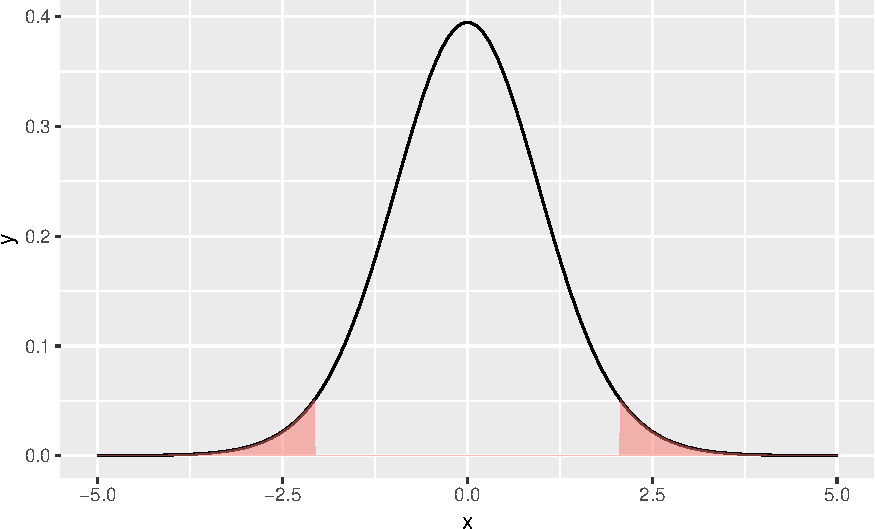
\includegraphics[width=0.7\linewidth]{regression-analysis_files/figure-latex/b0rjt-1} 

}

\caption{Rejection region for $\beta_0$}\label{fig:b0rjt}
\end{figure}

More importantly, we test \(\beta_1\) which means slope

\[H_0 : \beta_1 = \alpha_1 \qquad \text{vs} \qquad H_1 : \beta_1 \neq \alpha_1\]

\begin{equation}
  T = \frac{\hat\beta_1 - \alpha_1}{\hat\sigma \sqrt{\frac{1}{S_{xx}}}} \stackrel{H_0}{\sim} t(n - 2)
  \label{eq:b1test}
\end{equation}

For this test statistic \eqref{eq:b1test},

\[\text{reject}\: H_0 \quad \text{if} \: \lvert T \rvert > t_{\frac{\alpha}{2}}(n - 2)\]

Looking at these two statistics, we can intuitively know the meaning. As \(\lvert \hat\beta_1 - \alpha_1 \rvert\) becomes larger, the data support \(H_1\).

\hypertarget{analysis-of-variance}{%
\section{Analysis of Variance}\label{analysis-of-variance}}

\hypertarget{useful-distributions}{%
\subsection{Useful distributions}\label{useful-distributions}}

In linear regression setting, we usually assume \(\epsilon_i \stackrel{iid}{\sim}N(0, \sigma^2)\). There are some useful distributions around Normal.

\BeginKnitrBlock{proposition}[$\chi^2$-distribution]
\protect\hypertarget{prp:chisq}{}{\label{prp:chisq} \iffalse (\(\chi^2\)-distribution) \fi{} }Square of standard normal follows \(\chi^2\)-distribution.

If \(Z \sim N(0, 1)\), then \(Z^2 \sim \chi^2(1)\)

If \(Z_i \stackrel{indep}{\sim}N(0, 1)\), then \(Z_1^2 + \cdots + Z_n^2 \sim \chi^2(n)\)
\EndKnitrBlock{proposition}

\BeginKnitrBlock{proposition}[t-distribution]
\protect\hypertarget{prp:tdist}{}{\label{prp:tdist} \iffalse (t-distribution) \fi{} }Let \(Z \sim N(0, 1) \perp\!\!\!\perp V \sim \chi^2(m)\). Then

\[T = \frac{Z}{\sqrt{V / m}} \sim t(m)\]
\EndKnitrBlock{proposition}

\BeginKnitrBlock{proposition}[F-distribution]
\protect\hypertarget{prp:fdist}{}{\label{prp:fdist} \iffalse (F-distribution) \fi{} }Let \(V \sim \chi^2(m) \perp\!\!\!\perp W \sim \chi^2(n)\). Then

\[F = \frac{V / m}{W / n} \sim F(m, n)\]
\EndKnitrBlock{proposition}

Also, there is \emph{non-central analogue} of these three distributions, i.e.~starting from \(Z \sim N(\mu, 1)\).

\BeginKnitrBlock{proposition}[Noncentral $\chi^2$-distribution]
\protect\hypertarget{prp:nonchi}{}{\label{prp:nonchi} \iffalse (Noncentral \(\chi^2\)-distribution) \fi{} }Square of scaled normal follows non-central \(\chi^2\)-distribution.

If \(Z_i \stackrel{indep}{\sim}N(\mu_i, 1)\), then \(Z_1^2 + \cdots + Z_n^2 \sim \chi^2(n, \sum\limits_{i = 1}^n \mu_i^2)\)

\(\sum\limits_{i = 1}^n \mu_i^2\) is called a non-central parameter.
\EndKnitrBlock{proposition}

\BeginKnitrBlock{proposition}[Noncentral t-distribution]
\protect\hypertarget{prp:nontdist}{}{\label{prp:nontdist} \iffalse (Noncentral t-distribution) \fi{} }Let \(X \sim N(\mu, 1) \perp\!\!\!\perp V \sim \chi^2(m)\). Then

\[T = \frac{Z}{\sqrt{V / m}} \sim t(m, \mu)\]

\(\mu\) is called a non-central parameter.
\EndKnitrBlock{proposition}

\BeginKnitrBlock{proposition}[Noncentral F-distribution]
\protect\hypertarget{prp:nonfdist}{}{\label{prp:nonfdist} \iffalse (Noncentral F-distribution) \fi{} }Let \(V \sim \chi^2(m, \delta) \perp\!\!\!\perp W \sim \chi^2(n)\). Then

\[F = \frac{V / m}{W / n} \sim F(m, n, \delta)\]

\(\delta\) is called a non-central parameter.
\EndKnitrBlock{proposition}

\hypertarget{quadratic-form}{%
\subsection{Quadratic form}\label{quadratic-form}}

Now we can determine the distributions of various quadratic forms. The reason we are taking care of this is ANOVA deals with sum of squares, i.e.~quadratic form. See Corollary \ref{cor:projss} for this.

\begin{itemize}
\tightlist
\item
  \(SST = \mathbf{Y}^T(I - \Pi_{\mathbf{1}})\mathbf{Y}\)
\item
  \(SSR = \mathbf{Y}^T(\Pi_X - \Pi_{\mathbf{1}})\mathbf{Y}\)
\item
  \(SSE = \mathbf{Y}^T(I - \Pi_X)\mathbf{Y}\)
\end{itemize}

\BeginKnitrBlock{theorem}[Idempotent and symmetric]
\protect\hypertarget{thm:idem}{}{\label{thm:idem} \iffalse (Idempotent and symmetric) \fi{} }Let \(A \in \mathbb{R}^{k \times k}\) be idempotent and symmetric. Then

\begin{enumerate}[label=(\alph*)]
  \item $A^n$ is also idempotent \label{itm:idemone}
  \item $I - A$ is also idempotent \label{itm:idemtwo}
  \item Every eigenvalue of $A$ is either $0$ or $1$ so that $tr(A) = rank(A)$ \label{itm:idemthree}
\end{enumerate}
\EndKnitrBlock{theorem}

\BeginKnitrBlock{proof}
\iffalse{} {Proof. } \fi{}\(\ref{itm:idemone}\) and \(\ref{itm:idemtwo}\) are trivial.

\[(A^n)^2 = (A^2)^n = A^n\]

\[(I - A)^2 = I - 2A + A^2 = I - A\]

\(\ref{itm:idemthree}\)

Fix \(\lambda\) an eigenvalue of \(A\). Let \(\mathbf{v} \neq \mathbf{0}\) be the corresponding eigenvector.

By definition,

\[A\mathbf{v} = \lambda \mathbf{v}\]

Then

\[A^2\mathbf{v} = \lambda(A\mathbf{v}) = \lambda^2\mathbf{v}\]

and so \(\lambda^2\) is eigenvalue of \(A^2\).

Since \(A^2 = A\),

\[\lambda = \lambda^2\]

Hence,

\[\lambda = 0 \:\text{or}\: 1\]

Note that for every matrix and its eigenvalues \(\lambda_j\)

\[tr(A) = \sum_{j = 1}^p \lambda_j, \quad rank(A) = \text{the number of non-zero}\: \lambda_j\]

Since \(\lambda = 0, 1\) of A,

\[tr(A) = rank(A)\]
\EndKnitrBlock{proof}

\BeginKnitrBlock{proposition}[Independence]
\protect\hypertarget{prp:quadmvn}{}{\label{prp:quadmvn} \iffalse (Independence) \fi{} }Assume \(\mathbf{Y} \sim MVN(\mathbf\mu, \Sigma)\). Then

\begin{enumerate}[label=(\roman*)]
  \item If $A$ and $B$ are symmetric, $$Y^T AY \perp\!\!\!\perp Y^T BY \Leftrightarrow A\Sigma B = 0$$
  \item If $A$ is symmetric, $$Y^T AY \perp\!\!\!\perp BY \Leftrightarrow B\Sigma A = 0$$
\end{enumerate}
\EndKnitrBlock{proposition}

\BeginKnitrBlock{theorem}[Distribution of quadratic form]
\protect\hypertarget{thm:quaddist}{}{\label{thm:quaddist} \iffalse (Distribution of quadratic form) \fi{} }Assume that \(\mathbf{Y} \sim MVN(\mathbf\mu, I)\) and that \(A\) is symmetric and idempotent. Then

\[Y^T AY \sim \chi^2(K, \delta)\]

where \(K = rank(A)\) and \(\delta = \boldsymbol\mu^T A \boldsymbol\mu\). Furthermore,

\[
\begin{cases}
  E(Y^T AY) = K + \delta \\
  Var(Y^T AY) = 2(K + 2\delta)
\end{cases}
\]
\EndKnitrBlock{theorem}

\BeginKnitrBlock{corollary}[Inner product of standard normal vector]
\protect\hypertarget{cor:mvnchi}{}{\label{cor:mvnchi} \iffalse (Inner product of standard normal vector) \fi{} }Let \(\mathbf{Z} = (Z_1, \ldots, Z_n)^T \sim MVN(\mathbf{0}, I_n)\). Then

\[\mathbf{Z}^T\mathbf{Z} = \sum_{i = 1}^n Z_i^2 \sim \chi^2(n)\]
\EndKnitrBlock{corollary}

\BeginKnitrBlock{proof}
\iffalse{} {Proof. } \fi{}From Theorem \ref{thm:quaddist} point of view,

\[\mathbf{Z}^T\mathbf{Z} = \mathbf{Z}^T I_n \mathbf{Z}\]

Thus,

\[K = rank(I_n) = n\]

\[\delta = \mathbf{0}\]
\EndKnitrBlock{proof}

Using the above facts, we can now show distributions of sums of squares. First recall that

\[\mathbf{Y} \sim MVN(X\boldsymbol\beta, \sigma^2 I)\]

\BeginKnitrBlock{proposition}[Distribution of SSE]
\protect\hypertarget{prp:ssedist}{}{\label{prp:ssedist} \iffalse (Distribution of SSE) \fi{} }\[\frac{SSE}{\sigma^2} \sim \chi^2(n - 2, 0)\]
\EndKnitrBlock{proposition}

\BeginKnitrBlock{proof}
\iffalse{} {Proof. } \fi{}From Corollary \ref{cor:projss}, write

\[\frac{SSE}{\sigma^2} = \bigg(\frac{\mathbf{Y}}{\sigma}\bigg)^T (I - \Pi_X) \bigg(\frac{\mathbf{Y}}{\sigma}\bigg)\]

Note that

\[\frac{\mathbf{Y}}{\sigma} \sim MVN(\frac{1}{\sigma}X\boldsymbol\beta, I)\]

Since \(I - \Pi_X\) is idempotent and symmetric,

\[K = rank(I - \Pi_X) = tr(I - \Pi_X) = n - rank(\Pi_X) = n - 2\]

\begin{equation} \label{eq:delta1}
  \begin{split}
    \delta & = \bigg(\frac{X\boldsymbol\beta}{\sigma}\bigg)^T (I - \Pi_X) \bigg(\frac{X\boldsymbol\beta}{\sigma}\bigg) \\
    & = \frac{\boldsymbol\beta^TX^TX\boldsymbol\beta}{\sigma^2} - \frac{(\boldsymbol\beta^TX^T)X(X^TX)^{-1}X^T(X\boldsymbol\beta)}{\sigma^2} \\
    & = \frac{\boldsymbol\beta^TX^TX\boldsymbol\beta}{\sigma^2} - \frac{\boldsymbol\beta^TX^TX\boldsymbol\beta}{\sigma^2} \\
    & = 0
  \end{split}
\end{equation}

Hence,

\[\frac{SSE}{\sigma^2} \sim \chi^2(n - 2, 0)\]
\EndKnitrBlock{proof}

In case of \(SSE\), it always follows \(\chi^2(n - 2)\) no matter what \(H_0\) is. However, \(SSR\) and \(SST\) depend on \(\beta_1\) that we want to test.

\BeginKnitrBlock{proposition}[Distribution of SSR]
\protect\hypertarget{prp:ssrdist}{}{\label{prp:ssrdist} \iffalse (Distribution of SSR) \fi{} }\[\frac{SSR}{\sigma^2} \sim \chi^2(1, \delta)\]

where \(\delta = \frac{1}{\sigma^2}\sum\limits_{i = 1}^n (x_i - \overline{x})^2 \beta_1^2 = \frac{S_{xx}\beta_1^2}{\sigma^2}\)
\EndKnitrBlock{proposition}

\BeginKnitrBlock{proof}
\iffalse{} {Proof. } \fi{}From Corollary \ref{cor:projss}, write

\[\frac{SSR}{\sigma^2} = \bigg(\frac{\mathbf{Y}}{\sigma}\bigg)^T (\Pi_X - \Pi_{\mathbf{1}}) \bigg(\frac{\mathbf{Y}}{\sigma}\bigg)\]

Note that \(\Pi_X - \Pi_{\mathbf{1}}\) is symmetric idempotent. One proceeds in a similar way.

\[K = rank(\Pi_X - \Pi_{\mathbf{1}}) = tr(\Pi_X - \Pi_{\mathbf{1}}) = rank(\Pi_X) - rank(\Pi_{\mathbf{1}}) = 2 - 1 = 1\]

\begin{equation*}
  \begin{split}
    \delta & = \bigg(\frac{X\boldsymbol\beta}{\sigma}\bigg)^T (\Pi_X - \Pi_{\mathbf{1}}) \bigg(\frac{X\boldsymbol\beta}{\sigma}\bigg) \qquad \because \frac{\mathbf{Y}}{\sigma} \sim MVN(\frac{1}{\sigma}X\boldsymbol\beta, I) \\
    & = \frac{\boldsymbol\beta^T \Big\{ X^T(\Pi_X - \Pi_{\mathbf{1}})X \Big\} \boldsymbol\beta }{\sigma^2}
  \end{split}
\end{equation*}

Since \(\mathbf{1} \in Col(X)\),

\[\Pi_X \mathbf{1} = \mathbf{1}\]

It gives that

\begin{equation} \label{eq:ssrquad1}
  \mathbf{1}^T(\Pi_X - \Pi_{\mathbf{1}})\mathbf{1} = 0
\end{equation}

If \(\mathbf{x} \neq \mathbf{1}\), then we have

\begin{equation} \label{eq:ssrquad2}
  \mathbf{x}^T(\Pi_X - \Pi_{\mathbf{1}})\mathbf{x} = \sum_{i = 1}^n (x_i - \overline{x})^2 = S_{xx}
\end{equation}

Recall that

\[\overline{x}\mathbf{1} = \mathbf{1}(\mathbf{1}^T\mathbf{1})^{-1}\mathbf{1}^T\mathbf{x} = \Pi_{\mathbf{1}}\mathbf{x}\]

Then we have

\begin{equation} \label{eq:ssrquad3}
  \mathbf{1}^T(\Pi_X - \Pi_{\mathbf{1}})\mathbf{x} = \sum x_i - n \overline{x} = 0
\end{equation}

By symmetry,

\begin{equation} \label{eq:ssrquad4}
  \mathbf{x}^T(\Pi_X - \Pi_{\mathbf{1}})\mathbf{1} = n \overline{x} - \sum x_i = 0
\end{equation}

Hence by partitioning \(X = [\mathbf{1} \mid \mathbf{x}]\),

\begin{equation} \label{eq:delta2}
  \begin{split}
    \delta & = \frac{\boldsymbol\beta^T \Big\{ [\mathbf{1} \mid \mathbf{x}]^T(\Pi_X - \Pi_{\mathbf{1}})[\mathbf{1} \mid \mathbf{x}] \Big\} \boldsymbol\beta }{\sigma^2} \\
    & = \frac{\boldsymbol\beta^T \begin{bmatrix} \eqref{eq:ssrquad1} & \eqref{eq:ssrquad3} \\ \eqref{eq:ssrquad4} & \eqref{eq:ssrquad2} \end{bmatrix} \boldsymbol\beta}{\sigma^2} \\
    & = \frac{\boldsymbol\beta^T \begin{bmatrix} 0 & 0 \\ 0 & S_{xx} \end{bmatrix} \boldsymbol\beta}{\sigma^2} \\
    & = \frac{S_{xx}\beta_1^2}{\sigma^2}
  \end{split}
\end{equation}
\EndKnitrBlock{proof}

\BeginKnitrBlock{proposition}[Independence]
\protect\hypertarget{prp:ssind}{}{\label{prp:ssind} \iffalse (Independence) \fi{} }SSE and SSR are independent, i.e.

\[SSE \perp\!\!\!\perp SSR\]
\EndKnitrBlock{proposition}

\BeginKnitrBlock{proof}
\iffalse{} {Proof. } \fi{}Note that both \(SSE\) and \(SSR\) are quadratic forms of \(\mathbf{Y} \sim MVN(X\boldsymbol\beta, \sigma^2 I)\) and that each \(I - \Pi_X\) and \(\Pi_X - \Pi_{\mathbf{1}}\) is symmetric. Then from Proposition \ref{prp:quadmvn},

Claim: \((I - \Pi_X)(\sigma^2I)(\Pi_X - \Pi_{\mathbf{1}}) = 0\), i.e.~\((I - \Pi_X)(\Pi_X - \Pi_{\mathbf{1}}) = 0\)

It is obvious that

\[\Pi_X\Pi_{\mathbf{1}} = \Pi_{\mathbf{1}}\]

Then

\begin{equation*}
  \begin{split}
    (I - \Pi_X)(\Pi_X - \Pi_{\mathbf{1}}) & = \Pi_X - \Pi_{\mathbf{1}} - \Pi_X^2 + \Pi_X\Pi_{\mathbf{1}} \\
    & = \Pi_X - \Pi_{\mathbf{1}} - \Pi_X + \Pi_{\mathbf{1}} \qquad \because \text{idempotent} \\
    & = 0
  \end{split}
\end{equation*}

This completes the proof.
\EndKnitrBlock{proof}

\BeginKnitrBlock{proposition}[Independence]
\protect\hypertarget{prp:ssbind}{}{\label{prp:ssbind} \iffalse (Independence) \fi{} }SSE and \((\hat\beta_0, \hat\beta_1)\) are independent, i.e.

\[SSE \perp\!\!\!\perp(\hat\beta_0, \hat\beta_1)^T\]
\EndKnitrBlock{proposition}

\BeginKnitrBlock{proof}
\iffalse{} {Proof. } \fi{}Note that

\[\boldsymbol{\hat\beta}= (\hat\beta_0, \hat\beta_1)^T = (X^TX)^{-1}X^T\mathbf{Y}\]

Since \(I - \Pi_X\) of \(SSE\) is symmetric, from Proposition \ref{prp:quadmvn},

Claim: \(((X^TX)^{-1}X^T)(\sigma^2I)(I - \Pi_X) = 0\), i.e.~\(((X^TX)^{-1}X^T)(I - \Pi_X) = 0\)

Since \(\Pi_X = X(X^TX)^{-1}X^T\),

\begin{equation*}
  \begin{split}
    ((X^TX)^{-1}X^T)(I - \Pi_X) & = (X^TX)^{-1}X^T - (X^TX)^{-1}X^TX(X^TX)^{-1}X^T \\
    & = (X^TX)^{-1}X^T - (X^TX)^{-1}X^T \\
    & = 0
  \end{split}
\end{equation*}

This completes the proof.
\EndKnitrBlock{proof}

\BeginKnitrBlock{proposition}[Distribution of SST]
\protect\hypertarget{prp:sstdist}{}{\label{prp:sstdist} \iffalse (Distribution of SST) \fi{} }\[\frac{SST}{\sigma^2} \sim \chi^2(n - 1, \delta)\]

where \(\delta = \sum\limits_{i = 1}^n (x_i - \overline{x})^2 \beta_1^2 = \frac{S_{xx}\beta_1^2}{\sigma^2}\)
\EndKnitrBlock{proposition}

\BeginKnitrBlock{proof}
\iffalse{} {Proof. } \fi{}It proceedes in a similary way from Corollary \ref{cor:projss}

\[\frac{SST}{\sigma^2} = \bigg(\frac{\mathbf{Y}}{\sigma}\bigg)^T (I - \Pi_{\mathbf{1}}) \bigg(\frac{\mathbf{Y}}{\sigma}\bigg)\]

Since \(I - \Pi_{\mathbf{1}}\) is symmetric idempotent,

\[K = rank(I - \Pi_{\mathbf{1}}) = tr(I - \Pi_{\mathbf{1}}) = n - rank(\Pi_{\mathbf{1}}) = n - 1\]

Since \(\mathbf{1} \in sp( \{ \mathbf{1} \})\),

\[\Pi_{\mathbf{1}} \mathbf{1} = \mathbf{1}\]

Hence,

\begin{equation*}
  \begin{split}
    \delta & = \bigg(\frac{X\boldsymbol\beta}{\sigma}\bigg)^T (I - \Pi_{\mathbf{1}}) \bigg(\frac{X\boldsymbol\beta}{\sigma}\bigg) \\
    & = \frac{S_{xx}\beta_1^2}{\sigma^2} \qquad \because \eqref{eq:delta1} \:\text{and}\: \eqref{eq:delta2} 
  \end{split}
\end{equation*}
\EndKnitrBlock{proof}

\hypertarget{anova-for-testing-significance-of-regression}{%
\subsection{ANOVA for testing significance of regression}\label{anova-for-testing-significance-of-regression}}

Recall that

\[SST = SSR + SSE\]

\begin{itemize}
\tightlist
\item
  \(SST\): the variation of a response itself
\item
  \(SSR\): the variation of a response \emph{explained by the model}
\item
  \(SSE\): the variation of a response that \emph{cannot be explained by the model}
\end{itemize}

As mentioned in section \ref{decompsst}, whether the model is useful or not can depend on the proportion of \(SSR\) versus \(SSE\) in constant \(SST\). When \(SSR\) is large compared to \(SSE\), we can say that the model is good. On the other hand, when \(SSR\) is not large, the model might be poor. This is what \(R^2\) measures intuitively.

However, this direct comparison somtimes does not work in many times. Both \(SSR\) and \(SSE\) comes from different distribution, which have different degrees of freedom. So we \emph{compare standardized versions}, i.e.~divided by the degrees of freedom.

\BeginKnitrBlock{definition}[Degrees of freedom]
\protect\hypertarget{def:dof}{}{\label{def:dof} \iffalse (Degrees of freedom) \fi{} }Degrees of freedom of each sum of squares is

\[df = \text{the number of deviation} - \text{the number of linear constraints}\]
\EndKnitrBlock{definition}

\BeginKnitrBlock{corollary}[df of SS]
\protect\hypertarget{cor:dfss}{}{\label{cor:dfss} \iffalse (df of SS) \fi{} }\(df\) of each sum of square is computed as

\begin{enumerate}[label=(\alph*)]
  \item $df(SST) = n - 1$ \label{itm:dfssone}
  \item $df(SSR) = 1$ \label{itm:dfsstwo}
  \item $df(SSE) = n - 2$ \label{itm:dfssthree}
\end{enumerate}
\EndKnitrBlock{corollary}

\BeginKnitrBlock{proof}
\iffalse{} {Proof. } \fi{}\(\ref{itm:dfssone}\)

Since \(\sum (Y_i - \overline{Y}) = 0\), we have \(1\) linear constraints. Thus,

\[df(SST) = n - 1\]

\(\ref{itm:dfsstwo}\)

Note that \(\hat{Y_i} - \overline{Y} = \hat\beta_1(x_i - \overline{x})\)

where \(\sum (x_i - \overline{x}) = 0\).

Thus,

\[df(SSR) = n - (n - 1) = 1\]

\(\ref{itm:dfssthree}\)

From Example \ref{exm:usingnormal}, \(\sum (Y_i - \hat{Y_i}) = 0\) and \(\sum x_i (Y_i - \hat{Y_i}) = 0\).

Thus,

\[df(SSE) = n - 2\]
\EndKnitrBlock{proof}

Dividing sum of squares in \(df\), we can standardize it.

\BeginKnitrBlock{definition}[Mean square]
\protect\hypertarget{def:ms}{}{\label{def:ms} \iffalse (Mean square) \fi{} }Mean square is a sum of square \(SS\) divided by its degree of freedom \(df\)

\[MS := \frac{SS}{df}\]
\EndKnitrBlock{definition}

Using the values of corollary \ref{cor:dfss} we can define each mean square for \(SSR\) and \(SSE\).

\BeginKnitrBlock{definition}[Regression mean square]
\protect\hypertarget{def:msr}{}{\label{def:msr} \iffalse (Regression mean square) \fi{} }\[MSR := \frac{SSR}{1} = SSR\]
\EndKnitrBlock{definition}

From Proposition \ref{prp:ssrdist}, the following corollary can be drawn.

\BeginKnitrBlock{corollary}[Distribution of MSR]
\protect\hypertarget{cor:msrdist}{}{\label{cor:msrdist} \iffalse (Distribution of MSR) \fi{} }Under \(H_0: \beta_1 = 0\),

\[\frac{SSR}{\sigma^2} \stackrel{H_0}{\sim} \chi^2(1)\]
\EndKnitrBlock{corollary}

Now standardize residual sum of square.

\BeginKnitrBlock{definition}[Residual mean square]
\protect\hypertarget{def:mse}{}{\label{def:mse} \iffalse (Residual mean square) \fi{} }\[MSE := \frac{SSE}{n - 2}\]
\EndKnitrBlock{definition}

From Proposition \ref{prp:ssrdist}, we can construct same statistic. In fact, \(\frac{SSE}{\sigma^2}\) follows \(\chi^2(n - 2)\) whether or not \(\beta_1\) is zero. Its \(\delta = 0\).

\BeginKnitrBlock{corollary}[Distribution of MSE]
\protect\hypertarget{cor:msedist}{}{\label{cor:msedist} \iffalse (Distribution of MSE) \fi{} }\[\frac{SSE}{\sigma^2} \sim \chi^2(n - 2)\]
\EndKnitrBlock{corollary}

Finally, we can now use Proposition \ref{prp:fdist} so that

\[
F \equiv \frac{MSR}{MSE} = \frac{\frac{SSE / \sigma^2 \sim \chi^2(1)}{1}}{\frac{SSR / \sigma^2 \stackrel{H_0}{\sim}\chi^2(n - 2)}{n - 2}} \stackrel{H_0}{\sim}F(1, n - 2)
\]

By construction, this test statistic is used for

\[H_0: \beta_1 = 0\]

which means that the predictor does not explain the response anything. In other words, we are testing that

\begin{equation}
  H_0: \text{Model is not useful at all} \qquad \text{vs} \qquad H_1: \text{Model can explain data}
  \label{eq:goodfit}
\end{equation}

\BeginKnitrBlock{remark}[F statistic on testing significance]
\iffalse{} {Remark (F statistic on testing significance). } \fi{}Null hypothesis \eqref{eq:goodfit} can be tested with \(F\)-statistic.

\[F_0 = \frac{MSR}{MSE} = \frac{SSR / df(SSR)}{SSE / df(SSE)} \stackrel{H_0}{\sim}F(df(SSR), df(SSE))\]
\EndKnitrBlock{remark}

Here, it is

\[F_0 = \frac{SSR / 1}{SSE / (n - 2)}\]

Then we reject \(H_0\) if

\[F_0 > F_\alpha\bigg( df(SSR), df(SSE) \bigg)\]

\begin{figure}[H]

{\centering 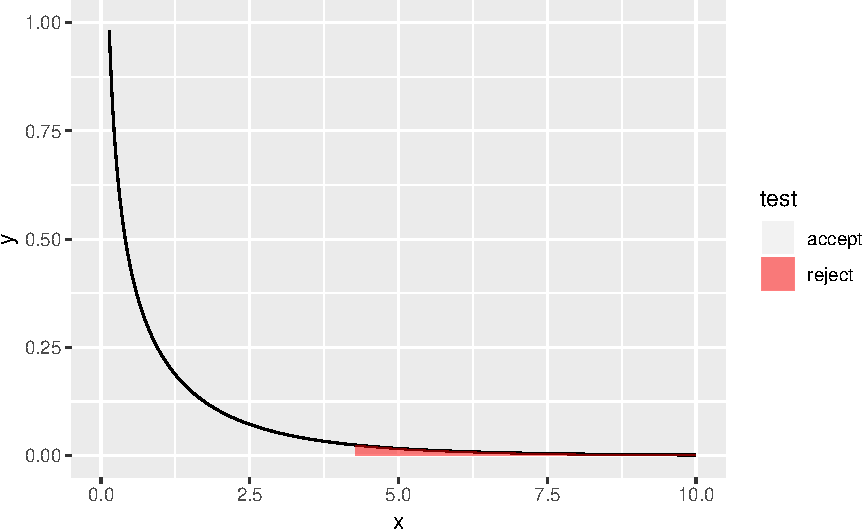
\includegraphics[width=0.7\linewidth]{regression-analysis_files/figure-latex/goodfitfig-1} 

}

\caption{Rejection region for significance testing}\label{fig:goodfitfig}
\end{figure}

\begin{Shaded}
\begin{Highlighting}[]
\KeywordTok{summary}\NormalTok{(delv_fit)}
\CommentTok{#> }
\CommentTok{#> Call:}
\CommentTok{#> lm(formula = y ~ x, data = delv)}
\CommentTok{#> }
\CommentTok{#> Residuals:}
\CommentTok{#>    Min     1Q Median     3Q    Max }
\CommentTok{#> -7.581 -1.874 -0.349  2.181 10.634 }
\CommentTok{#> }
\CommentTok{#> Coefficients:}
\CommentTok{#>             Estimate Std. Error t value Pr(>|t|)    }
\CommentTok{#> (Intercept)    3.321      1.371    2.42    0.024 *  }
\CommentTok{#> x              2.176      0.124   17.55  8.2e-15 ***}
\CommentTok{#> ---}
\CommentTok{#> Signif. codes:  0 '***' 0.001 '**' 0.01 '*' 0.05 '.' 0.1 ' ' 1}
\CommentTok{#> }
\CommentTok{#> Residual standard error: 4.18 on 23 degrees of freedom}
\CommentTok{#> Multiple R-squared:  0.93,   Adjusted R-squared:  0.927 }
\CommentTok{#> F-statistic:  308 on 1 and 23 DF,  p-value: 8.22e-15}
\end{Highlighting}
\end{Shaded}

This statistic is \texttt{F-statistic} included in \texttt{summary.lm()} output. This is saved as \texttt{\$fstatistic}.

\begin{Shaded}
\begin{Highlighting}[]
\KeywordTok{summary}\NormalTok{(delv_fit)}\OperatorTok{$}\NormalTok{fstatistic}
\CommentTok{#> value numdf dendf }
\CommentTok{#>   308     1    23}
\end{Highlighting}
\end{Shaded}

We usually summarize these statistic in table form, so called \emph{ANOVA table}.

\begin{longtable}[]{@{}cccccc@{}}
\toprule
Source & SS & df & MS & F & p-value\tabularnewline
\midrule
\endhead
Model & \(SSR\) & \(1\) & \(MSR\) & \(F_0\) & p-value\tabularnewline
Error & \(SSE\) & \(n - 2\) & \(MSE\) & &\tabularnewline
Total & \(SST\) & \(n - 1\) & & &\tabularnewline
\bottomrule
\end{longtable}

To get this table, just use \texttt{anova()} for \texttt{lm} object.

\begin{Shaded}
\begin{Highlighting}[]
\KeywordTok{anova}\NormalTok{(delv_fit)}
\CommentTok{#> Analysis of Variance Table}
\CommentTok{#> }
\CommentTok{#> Response: y}
\CommentTok{#>           Df Sum Sq Mean Sq F value  Pr(>F)    }
\CommentTok{#> x          1   5382    5382     308 8.2e-15 ***}
\CommentTok{#> Residuals 23    402      17                    }
\CommentTok{#> ---}
\CommentTok{#> Signif. codes:  0 '***' 0.001 '**' 0.01 '*' 0.05 '.' 0.1 ' ' 1}
\end{Highlighting}
\end{Shaded}

Since the last \texttt{Total} row is just sum of the model and error, the function does not give it. To use this table as \texttt{data.frame} more easily, just implement \texttt{broom::tidy} as before.

\begin{Shaded}
\begin{Highlighting}[]
\KeywordTok{anova}\NormalTok{(delv_fit) }\OperatorTok\StringTok{ }
\StringTok{  }\NormalTok{broom}\OperatorTok{::}\KeywordTok{tidy}\NormalTok{()}
\CommentTok{#> # A tibble: 2 x 6}
\CommentTok{#>   term         df sumsq meansq statistic   p.value}
\CommentTok{#>   <chr>     <int> <dbl>  <dbl>     <dbl>     <dbl>}
\CommentTok{#> 1 x             1 5382. 5382.       308.  8.22e-15}
\CommentTok{#> 2 Residuals    23  402.   17.5       NA  NA}
\end{Highlighting}
\end{Shaded}

Denote that here \emph{simple linear regression setting} \(F\)-statistic and \(t\)-statistic of Equation \eqref{eq:b1test} perform exactly same thing, \(H_0 : \beta_1 = 0\). In fact, we know that

\[F(1, k) \stackrel{d}{=} T_k^2\]

\BeginKnitrBlock{remark}
\iffalse{} {Remark. } \fi{}In the simple linear regression setting, \(F\)-test for significance and \(t\)-test for no slope are equivalent, i.e.~under \(H_0 : \beta_1 = 0\)

\[F_0 = \frac{\hat\beta_1 S_{xx}}{\hat\sigma^2} = \bigg( \frac{\hat\beta_1}{\hat\sigma / \sqrt{S_{xx}}} \bigg) = T_0^2\]
\EndKnitrBlock{remark}

\hypertarget{multiple}{%
\chapter{Multiple Linear Regression}\label{multiple}}

\hypertarget{model-1}{%
\section{Model}\label{model-1}}

\begin{Shaded}
\begin{Highlighting}[]
\NormalTok{(cem <-}\StringTok{ }\NormalTok{MPV}\OperatorTok{::}\NormalTok{cement }\OperatorTok\StringTok{ }\KeywordTok{tbl_df}\NormalTok{())}
\CommentTok{#> # A tibble: 13 x 5}
\CommentTok{#>        y    x1    x2    x3    x4}
\CommentTok{#>    <dbl> <dbl> <dbl> <dbl> <dbl>}
\CommentTok{#>  1  78.5     7    26     6    60}
\CommentTok{#>  2  74.3     1    29    15    52}
\CommentTok{#>  3 104.     11    56     8    20}
\CommentTok{#>  4  87.6    11    31     8    47}
\CommentTok{#>  5  95.9     7    52     6    33}
\CommentTok{#>  6 109.     11    55     9    22}
\CommentTok{#>  7 103.      3    71    17     6}
\CommentTok{#>  8  72.5     1    31    22    44}
\CommentTok{#>  9  93.1     2    54    18    22}
\CommentTok{#> 10 116.     21    47     4    26}
\CommentTok{#> 11  83.8     1    40    23    34}
\CommentTok{#> 12 113.     11    66     9    12}
\CommentTok{#> 13 109.     10    68     8    12}
\end{Highlighting}
\end{Shaded}

Above is a data set about cement and concerning four ingredients from the \citet{Montgomery:2015aa} textbook.

\begin{itemize}
\tightlist
\item
  \texttt{y}: heat evolved in calories per gram of cement
\item
  \texttt{x1}: tricalcium aluminate
\item
  \texttt{x2}: tricalcium silicate
\item
  \texttt{x3}: tetracalcium alumino ferrite
\item
  \texttt{x4}: dicalcium silicate
\end{itemize}

Given data \((x_{11}, x_{12}, \ldots, x_{1p}, Y_1), \ldots, (x_{n1}, x_{n2}, \ldots, x_{np}, Y_n)\) (\(p = 4\)), we try to fit linear regression model

\[Y_i = \beta_0 + \beta_1 x_{i1} + \cdots + \beta_p x_{ip} + \epsilon_{i}\]

with

\[\epsilon_i \stackrel{iid}{\sim}(0, \sigma^2)\]

Compared to simple linear regression problem \ref{simple}, we have more parameters for coefficients

\[(\beta_0, \beta_1, \ldots, \beta_p, \sigma^2)\]

Each \(\beta_j\) is a change of \(Y\) when each predictor variable \(x_j\) increases in 1 unit while the others fixed. In this part, we use \emph{matrix notation}. Extending our former matrix work \ref{matnot},

\[
\underset{\huge \mathbf{Y}}{\begin{bmatrix}
  Y_1 \\
  Y_2 \\
  \vdots \\
  Y_n
\end{bmatrix}} = \underset{\huge X}{\begin{bmatrix}
  1 & x_{11} & \cdots & x_{1p} \\
  1 & x_{21} & \cdots & x_{2p} \\
  \vdots & \vdots & \vdots & \vdots \\
  1 & x_{n1} & \cdots & x_{np}
\end{bmatrix}} \underset{\huge \boldsymbol\beta}{\begin{bmatrix}
  \beta_0 \\
  \vdots \\
  \beta_p
\end{bmatrix}} + \underset{\huge \E}{\begin{bmatrix}
  \epsilon_1 \\
  \epsilon_2 \\
  \vdots \\
  \epsilon_n
\end{bmatrix}}
\]

where \(\epsilon_i\) are i.i.d., and

\[E \E = \mathbf{0}\]

\[Var \E = \sigma^2 I\]

\hypertarget{least-square-estimation}{%
\section{Least Square Estimation}\label{least-square-estimation}}

Write \(\boldsymbol\beta \equiv (\beta_1, \ldots, \beta_p)^T \in \mathbb{R}^{p + 1}\). Extend Equation \eqref{eq:qmatrix}.

\begin{equation}
  \begin{split}
    \boldsymbol{\hat\beta}& = \argmin_{ \boldsymbol\beta\in \mathbb{R}^{p + 1}} \sum_{i = 1}^n (Y_i - \beta_0 - \beta_1 x_{i1} - \cdots - \beta_p x_{ip})^2 \\
    & = \argmin_{ \boldsymbol\beta\in \mathbb{R}^{p + 1}} \lVert \mathbf{Y} - \beta_0 \mathbf{1} - \beta_1 \mathbf{x}_1 - \cdots - \beta_p \mathbf{x}_p \rVert^2 \\
    & = \argmin_{ \boldsymbol\beta\in \mathbb{R}^{p + 1}} \lVert \mathbf{Y} - X \boldsymbol\beta\rVert^2
  \end{split}
  \label{eq:qmultiple}
\end{equation}

As discussed, the solution \(\boldsymbol{\hat\beta}\) is related to the projection. \(X\boldsymbol{\hat\beta}\) is a projection of \(\mathbf{Y}\) onto \(Col(X)\).

\hypertarget{normal-equation}{%
\subsection{Normal equation}\label{normal-equation}}

Now recap the section \ref{solproj}. Fundamental subspaces theorem \ref{thm:fundsub} implies that

\[\mathbf{Y} - X \boldsymbol{\hat\beta}\in Col(X)^{\perp} = N(X^T)\]

From the second part of subset, i.e.~\(N(X^T)\), we now have \emph{Normal equation}

\begin{equation}
  X^T(\mathbf{Y} - X \boldsymbol{\hat\beta}) = \mathbf{0}
  \label{eq:multeq}
\end{equation}

This is equivalent to

\[X^T\mathbf{Y} = X^TX \boldsymbol{\hat\beta}\]

Hence, if \(X^T X\) is invertible, the equation gives unique solution

\[\boldsymbol{\hat\beta}= (X^TX)^{-1}X^T \mathbf{Y}\]

Our first question is when \(X^T X\) is invertible, and Theorem \ref{thm:fullrank} have said that it is when the model matrix \(X\) is full rank.

\BeginKnitrBlock{lemma}
\protect\hypertarget{lem:modelnnd}{}{\label{lem:modelnnd} }Let \(X \in \mathbb{R}^{n \times (p + 1)}\) be any model matrix. Then \(X^T X\) is always non-negative definite.

\[\forall \mathbf{v} \in \mathbb{R}^{p + 1} : \mathbf{v}^T(X^T X)\mathbf{v} \ge 0\]
\EndKnitrBlock{lemma}

\BeginKnitrBlock{proof}
\iffalse{} {Proof. } \fi{}Let \(\mathbf{v} \in \mathbb{R}^{p + 1}\). Then

\[\mathbf{v}^T(X^T X)\mathbf{v} = (X\mathbf{v})^T (X\mathbf{v}) = \lVert X\mathbf{v} \rVert^2 \ge 0\]
\EndKnitrBlock{proof}

This lemma can also prove our Theorem \ref{thm:fullrank}.

\BeginKnitrBlock{theorem}
\protect\hypertarget{thm:fullrank2}{}{\label{thm:fullrank2} }Let \(\mathbf{Y} = X\boldsymbol\beta\) inconsistent and let \(X \in \mathbb{R}^{n \times (p + 1)}\) with \(n > p + 1\).

If \(rank(X) = p + 1\), i.e.~full rank, then \(X^T X\) is invertible.
\EndKnitrBlock{theorem}

\BeginKnitrBlock{proof}
\iffalse{} {Proof. } \fi{}Let \(\mathbf{c} \in \mathbb{R}^{(p + 1)}\)

Suppose that \(X^T X\) is positive definite.

\begin{equation*}
  \begin{split}
    & \Leftrightarrow \mathbf{c}^TX^T X \mathbf{c} = 0 \quad \text{implies} \quad \mathbf{c} = \mathbf{0} \\
    & \Leftrightarrow X\mathbf{c} = \mathbf{0} \quad \text{implies} \quad \mathbf{c} = \mathbf{0} \\
    & \Leftrightarrow \text{columns of}\: X \:\text{linearly independent} \\
    & \Leftrightarrow rank(X) = p + 1
  \end{split}
\end{equation*}
\EndKnitrBlock{proof}

\hypertarget{orthogonal-decomposition}{%
\subsection{Orthogonal decomposition}\label{orthogonal-decomposition}}

\BeginKnitrBlock{theorem}
\protect\hypertarget{thm:orthonormal}{}{\label{thm:orthonormal} }Let \(Col(X)\) be a subspace of \(\mathbb{R}^n\), let \(\mathbf{Y} \in \mathbb{R}^n\), and let \(\{ \mathbf{u}_0, \ldots, \mathbf{u}_{p} \}\) be an orthonormal basis for \(Col(X)\). If

\[\mathbf{\hat{Y}} = \sum_{j = 0}^p \hat\beta_j \mathbf{u}_j\]

where

\[\hat\beta_j = \Pi(\mathbf{Y} \mid R(\mathbf{u}_j)) \quad \text{for each} \: i\]

then \(\mathbf{\hat{Y}} - \mathbf{Y} \in Col(X)^{\perp}\).
\EndKnitrBlock{theorem}

\BeginKnitrBlock{theorem}
\protect\hypertarget{thm:orthonormalproj}{}{\label{thm:orthonormalproj} }Under the hypothesis of Theorem \ref{thm:orthonormal}, \(\mathbf{\hat{Y}} \in Col(X)\) is the closest to \(\mathbf{Y}\) amongst its any element \(\mathbf{p}\), i.e.

\[\Vert \mathbf{p} - \mathbf{Y} \Vert > \Vert \mathbf{\hat{Y}} - \mathbf{Y} \Vert\]

for any \(\mathbf{p} \neq \mathbf{\hat{Y}}\) in \(Col(X)\)
\EndKnitrBlock{theorem}

In other words, projection of \(\mathbf{Y}\) onto \(Col(X)\), \(\mathbf{\hat{Y}}\) can be \emph{represented as sum of projections of} \(\mathbf{Y}\) \emph{onto each (orthogonal) individual variable}. Before looking at individual basis, consider two-block space.

Write

\[
X = \left[\begin{array}{c|ccc}
  1 & x_{11} & \cdots & x_{1p} \\
  1 & x_{21} & \cdots & x_{2p} \\
  \vdots & \vdots & \vdots & \vdots \\
  1 & x_{n1} & \cdots & x_{np}
\end{array}\right] = [\mathbf{1}, \mathbb{X}_A]
\]

Consider \(R(X)\), \(R(\mathbf{1})\), and \(R(\mathbb{X}_A)\).

To decompose subspace \(R(X)\), we try to orthogonalize \(\mathbf{1}\) and \(\mathbb{X}_A\). By Theorem \ref{thm:orthonormal}, we have

\[\mathbf{1} \perp \mathbb{X}_A - \Pi_{\mathbf{1}}\mathbb{X}_A\]

In fact, the right one \(\mathbb{X}_A - \Pi_{\mathbf{1}}\mathbb{X}_A\) is the \emph{residual after simple linear regression} \(\mathbb{X}_A\) onto \(\mathbf{1}\). We have seen in Figure \ref{fig:simpledraw2} of section \ref{matnot} that the \emph{residual is orthogonal to predictor vector}. In this procedure, we choose residual as new predictor instead of response in simple linear regression, i.e.~\(\mathbb{X}_A\). If this is done to individual predictor variables, it is called \emph{successive orthogonalization} and it will be coved next section with QR decomposition.

Theorem \ref{thm:dsum} implies that

\[R(X) = R(\mathbf{1}) \oplus R(\mathbb{X}_A - \Pi_{\mathbf{1}}\mathbb{X}_A)\]

\BeginKnitrBlock{theorem}[Orthogonal decomposition]
\protect\hypertarget{thm:orthdecomp}{}{\label{thm:orthdecomp} \iffalse (Orthogonal decomposition) \fi{} }Let \(X = [\mathbf{1}, \mathbb{X}_A]\). Then

\begin{enumerate}[label=(\roman*)]
  \item $$R(X) = R(\mathbf{1}) \oplus R(\mathbb{X}_A - \Pi_{\mathbf{1}}\mathbb{X}_A)$$ \label{itm:orthdecompone}
  \item $$\Pi(\cdot \mid R(X)) = \Pi(\cdot \mid R(\mathbf{1})) + \Pi(\cdot \mid R(\mathbb{X}_A - \Pi_{\mathbf{1}}\mathbb{X}_A))$$ \label{itm:orthdecomptwo}
\end{enumerate}
\EndKnitrBlock{theorem}

Write

\[\mathbb{X}_{A, \perp} := \mathbb{X}_A - \Pi_{\mathbf{1}}\mathbb{X}_A\]

Note that

\[\Pi_{\mathbf{1}} = \mathbf{1}(\mathbf{1}^T\mathbf{1})^{-1}\mathbf{1}^T = \frac{1}{n}\mathbf{1}\mathbf{1}^T\]

Then

\begin{equation}
  \begin{split}
    X\boldsymbol{\hat\beta} & = \hat\beta_0\mathbf{1} + \mathbb{X}_A\boldsymbol{\hat\beta}_A \\
    & = \hat\beta_0\mathbf{1} + (\mathbb{X}_{A, \perp} + \Pi_{\mathbf{1}}\mathbb{X}_A)\boldsymbol{\hat\beta}_A \\
    & = \Big(\hat\beta_0 + \frac{1}{n}\mathbf{1}^T\mathbb{X}_A\boldsymbol{\hat\beta}_A \Big)\mathbf{1} + \mathbb{X}_{A,\perp}\boldsymbol{\hat\beta}_A \qquad \because \hat\beta_0 + \frac{1}{n}\mathbf{1}^T\mathbb{X}_A\boldsymbol{\hat\beta}_A \in \mathbb{R}
  \end{split}
  \label{eq:blockfit}
\end{equation}

From (ii) of Theorem \ref{thm:orthdecomp},

\begin{equation}
  \begin{split}
    \Pi(\mathbf{Y} \mid R(X)) & = \Pi(\mathbf{Y} \mid R(\mathbf{1})) + \Pi(\mathbf{Y} \mid R(\mathbb{X}_{A,\perp})) \\
    & = \overline{Y}\mathbf{1} + \mathbb{X}_{A,\perp}(\mathbb{X}_{A,\perp}^T\mathbb{X}_{A,\perp})^{-1}\mathbb{X}_{A,\perp}^T\mathbf{Y}
  \end{split}
  \label{eq:decompfit}
\end{equation}

Since \(\mathbf{1} \perp \mathbb{X}_{A, \perp}\), Equations \eqref{eq:blockfit} and \eqref{eq:decompfit} imply that

\begin{equation}
  \begin{cases}
    \hat\beta_0 = \overline{Y} - \frac{1}{n}\mathbf{1}^T\mathbb{X}_A\boldsymbol{\hat\beta}_A \\
    \boldsymbol{\hat\beta}_A = (\mathbb{X}_{A,\perp}^T\mathbb{X}_{A,\perp})^{-1}\mathbb{X}_{A,\perp}^T\mathbf{Y}
  \end{cases}
  \label{eq:orthbeta}
\end{equation}

\begin{figure}[H]

{\centering 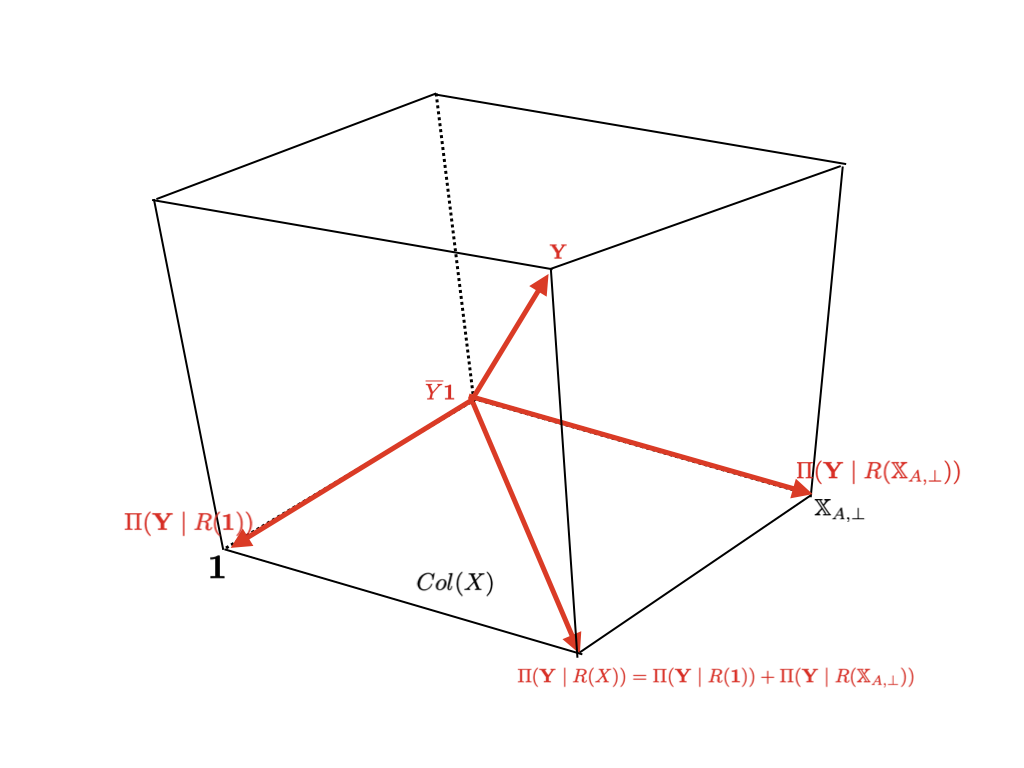
\includegraphics[width=0.7\linewidth]{images/multiple-orthogonal} 

}

\caption{Orthogonal decomposition of the column space and LSE}\label{fig:illdecomp}
\end{figure}

See Figure \ref{fig:illdecomp}. Two are orthogonal, so sum of projections onto them become LSE. In fact, \emph{each projection indicate each regression coefficient}. When we do not have orthogonal basis, however, each projection is nothing.

\begin{figure}[H]

{\centering 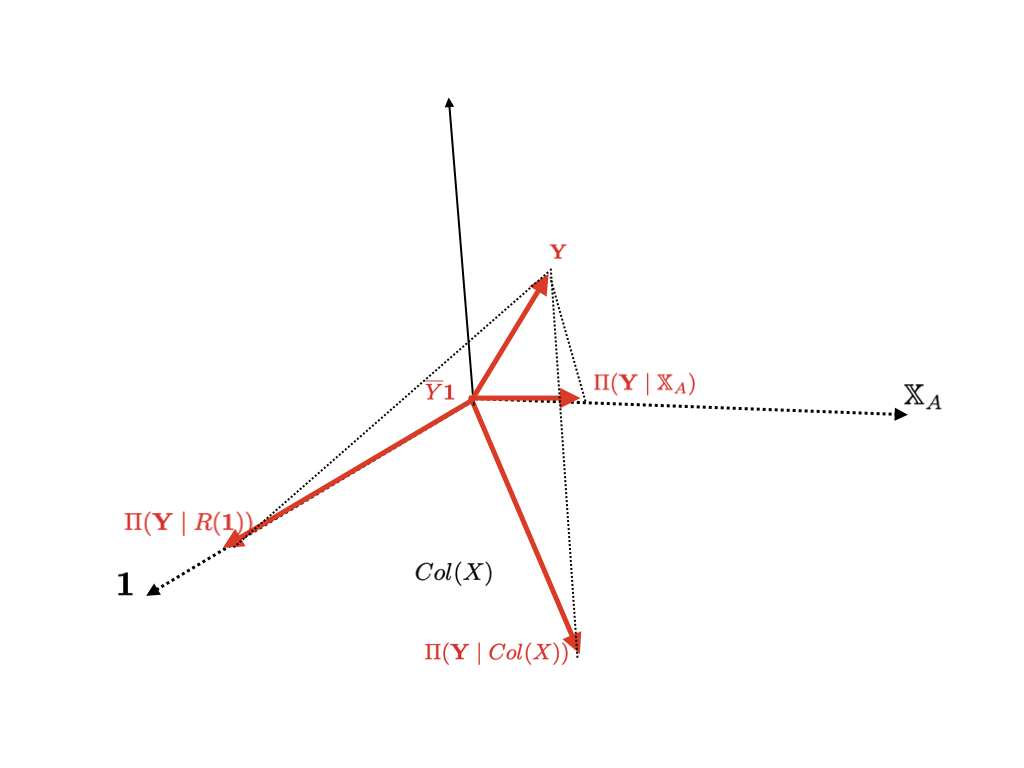
\includegraphics[width=0.7\linewidth]{images/multiple-nonorth} 

}

\caption{Non-orthongality}\label{fig:illdecomp2}
\end{figure}

So what we have done is orthogonalization.

\[\tilde{\mathbb{X}}_A = \Pi_{\mathbf{1}}\mathbb{X}_A + (\mathbb{X}_A - \Pi_{\mathbf{1}}\mathbb{X}_A)\]

\hypertarget{gram-schmidt-qr-factorization}{%
\subsection{Gram-Schmidt QR factorization}\label{gram-schmidt-qr-factorization}}

Let's briefly look at orthogonalization process. From Theorem \ref{thm:orthonormal}, we can derive following \emph{orthonormalization process}.

\BeginKnitrBlock{theorem}[Gram-Schmidt Process]
\protect\hypertarget{thm:gs}{}{\label{thm:gs} \iffalse (Gram-Schmidt Process) \fi{} }Let \(\{ \mathbf{x}_1, \ldots, \mathbf{x}_{p + 1} \}\) be a basis for the inner product space \(V\). Let

\[\mathbf{u}_1 = \bigg( \frac{1}{\lVert \mathbf{x}_1 \rVert} \bigg) \mathbf{x}_1\]

and define next \(\mathbf{u}_2, \ldots, \mathbf{u}_{p + 1}\) recursively by

\[\mathbf{u}_{k + 1} = \frac{1}{\lVert \mathbf{x}_{k + 1} - \mathbf{r}_k^{*} \rVert}(\mathbf{x}_{k + 1} - \mathbf{r}_k^{*})\]

for \(k = 1, \ldots, p\), where

\[\mathbf{r}_k^{*} = <\mathbf{x}_{k + 1}, \mathbf{u}_1> \mathbf{u}_1 + <\mathbf{x}_{k + 1}, \mathbf{u}_2 >\mathbf{u}_2 + \cdots + < \mathbf{x}_{k + 1}, \mathbf{u}_k > \mathbf{u}_k\]

is the projection of \(\mathbf{x}_{k + 1}\) onto \(sp(\{ \mathbf{u}_1, \ldots, \mathbf{u}_k \})\).

Hence, we get \(\{ \mathbf{u}_1, \ldots, \mathbf{u}_{p + 1} \}\) is an orthonormal basis for \(V\).
\EndKnitrBlock{theorem}

\begin{algorithm} \label{alg:alggs}
  \SetAlgoLined
  \SetKwInOut{Input}{input}
  \Input{basis $\{ \mathbf{x}_0, \ldots, \mathbf{x}_p \}$}
  Initialize $\mathbf{v}_0 = \mathbf{x}_0$\;
  \For{$k \leftarrow 1$ \KwTo $p$}{
    $\mathbf{u}_{k - 1} = \frac{\mathbf{v}_{k - 1}}{\lVert \mathbf{v}_{k - 1} \rVert}$\;
    $\mathbf{r}_k^{*} = <\mathbf{x}_{k + 1}, \mathbf{u}_0> \mathbf{u}_0 + <\mathbf{x}_{k + 1}, \mathbf{u}_1 >\mathbf{u}_1 + \cdots + < \mathbf{x}_{k + 1}, \mathbf{u}_k > \mathbf{u}_k$\;
    $\mathbf{v}_{k + 1} = \mathbf{x}_{k + 1} - \mathbf{r}_k^{*}$
  }
  $\mathbf{u}_p = \frac{\mathbf{v}_p}{\lVert \mathbf{v}_p \rVert}$
  \caption{Gram-schmidt process}
\end{algorithm}

Our interest is \(Col(X)\), and we can factorizae this model matrix so that it represents orthonormalization process \ref{thm:gs}.

\BeginKnitrBlock{theorem}[Gram-Schmidt QR factorization]
\protect\hypertarget{thm:gsqr}{}{\label{thm:gsqr} \iffalse (Gram-Schmidt QR factorization) \fi{} }Let \(X \in \mathbb{R}^{n \times (p + 1)}\). Then \(X\) can be factored into

\[X = QR\]

where \(Q \in \mathbb{R}^{n \times (p + 1)}\) is an orthogonal matrix, i.e.~its column vectors are orthonormal and \(R \in \mathbb{R}^{(p + 1) \times (p + 1)}\) is an upper triangular matrix whose diagonal entries are all positive.
\EndKnitrBlock{theorem}

\BeginKnitrBlock{proof}
\iffalse{} {Proof. } \fi{}Denote that this is just the representation of Gram-schmidt orthogonalization. Then it gives

\[\mathbf{u}_1 = \frac{\mathbf{x}_1}{\lVert \mathbf{x}_1 \rVert} \Rightarrow \mathbf{x}_1 = \lVert \mathbf{x}_1 \rVert \mathbf{u}_1\]

\begin{equation*}
  \begin{split}
    & \mathbf{v}_2 = \mathbf{x}_2 - <\mathbf{x}_2, \mathbf{u}_1> \mathbf{u}_1, \quad \mathbf{u}_2 = \frac{\mathbf{v}_2}{\lVert \mathbf{v}_2 \rVert} \\
    & \Rightarrow \mathbf{x}_2 = <\mathbf{x}_2, \mathbf{u}_1>\mathbf{u}_1 + \lVert \mathbf{v}_2 \rVert \mathbf{u}_2 \\
    & \Rightarrow \mathbf{x}_2 = \left[\begin{array}{c|c}
      \mathbf{u}_1 & \mathbf{u}_2
    \end{array}\right] \begin{bmatrix}
      <\mathbf{x}_2, \mathbf{u}_1> \\
      \lVert \mathbf{v}_2 \rVert
    \end{bmatrix}
  \end{split}
\end{equation*}

It procees in a simlar way to the others. Hence,

\begin{equation}
  \begin{split}
    X & = \begin{bmatrix} \mathbf{x}_1 & \cdots & \mathbf{x}_{p+1} \end{bmatrix} \\
    & = \begin{bmatrix}
      \mathbf{u}_1 & \mathbf{u}_2 & \cdots & \mathbf{u}_{p + 1}
    \end{bmatrix} \begin{bmatrix}
      \lVert \mathbf{v}_1 \rVert & < \mathbf{x}_2, \mathbf{u}_1> & < \mathbf{x}_3, \mathbf{u}_1> & \cdots & < \mathbf{x}_{p + 1}, \mathbf{u}_1> \\
      0 & \lVert \mathbf{v}_2 \rVert & < \mathbf{x}_3, \mathbf{u}_2> & \cdots & < \mathbf{x}_{p + 1}, \mathbf{u}_2> \\
      0 & 0 & \lVert \mathbf{v}_3 \rVert & \cdots & < \mathbf{x}_{p + 1}, \mathbf{u}_3> \\
      \vdots & \vdots & \vdots & \vdots & \vdots \\
      0 & 0 & 0 & 0 & \lVert \mathbf{v}_{p + 1} \rVert
    \end{bmatrix} \\
    & \equiv QR
  \end{split}
  \label{eq:qrrep}
\end{equation}
\EndKnitrBlock{proof}

Look again the equation in Theorem \ref{thm:gs}. In each process \(k\), the projection is done to the \((k - 1)\)-dimensional space. In other words, as process goes through, dimension increases. So we try to project each vector only in 1-dimension each step.

\BeginKnitrBlock{theorem}[Modified Gram-Schmidt Process]
\protect\hypertarget{thm:modgs}{}{\label{thm:modgs} \iffalse (Modified Gram-Schmidt Process) \fi{} }Let \(\{ \mathbf{x}_1, \ldots, \mathbf{x}_{p + 1} \}\) be a basis for the inner product space \(V\) and let \(\{ \mathbf{q}_1, \ldots, \mathbf{q}_{p + 1} \}\) be an orthonormal basis.

Set \(\mathbf{q}_1 = \frac{\mathbf{x}_1}{\lVert \mathbf{x}_1 \rVert}\). Then consider \(sp(\{ \mathbf{q}_1 \})\).

In the first step, make every \(\{ \mathbf{x}_2, \ldots, \mathbf{x}_{p + 1} \}\) orthogonal to \(\mathbf{q}_1\).

\[\mathbf{x}_k^{(1)} = \mathbf{x}_k - (\mathbf{q}_1^T \mathbf{x}_k)\mathbf{q}_1, \quad k = 2, \ldots, p + 1\]

So we get orthogonal set \(\{ \mathbf{q}_1, \mathbf{x}_2^{(1)}, \ldots, \mathbf{x}_{p + 1}^{(1)} \}\). Next, set \(\mathbf{q}_2 = \frac{\mathbf{x}^{(1)}}{\lVert \mathbf{x}_2^{(2)} \rVert}\). Consider \(sp(\{ \mathbf{q}_2 \})\). Since we have \(\mathbf{q}_1 \perp \mathbf{q}_2\),

\[\mathbf{x}_k^{(2)} = \mathbf{x}_k^{(1)} - (\mathbf{q}_2^T \mathbf{x}_k^{(1)})\mathbf{q}_2 \perp \mathbf{q}_2 , \quad k = 3, \ldots, p + 1\]

Thus, get \(\{ \mathbf{q}_1, \mathbf{q}_2, \mathbf{x}_3^{(2)}, \ldots, \mathbf{x}_{p + 1}^{(2)} \}\). \(\mathbf{q}_3, \ldots, \mathbf{q}_{p + 1}\) are successively determined in a similary way.

At the last step, set

\[\mathbf{q}_{p + 1} = \frac{\mathbf{x}_{p + 1}^{(p)}}{\lVert \mathbf{x}_{p + 1}^{(p)} \rVert}\]
\EndKnitrBlock{theorem}

Since each projection is done in 1-dimension, the algorithm becomes more understandable. Consider

\[
Q = \begin{bmatrix}
  \mathbf{q}_1 & \mathbf{q}_2 & \cdots \mathbf{q}_{p + 1}
\end{bmatrix} \in \mathbb{R}^{n \times (p + 1)} \quad \text{orthogonal}
\]

and

\[
R = [r_{kj}] = \begin{bmatrix}
  r_{11} & r_{12} & \cdots & r_{1,p+1} \\
  0 & r_{22} & \cdots & r_{2, p+1} \\
  0 & 0 & \cdots & r_{3,p+1} \\
  \vdots & \vdots & \vdots & \vdots \\
  0 & 0 & 0 & r_{p+1, p+1}
\end{bmatrix} \in \mathbb{R}^{(p+1) \times (p + 1)}
\]

We can perform \(QR\) factorization by following step.

\begin{algorithm} \label{alg:algqr}
  \SetAlgoLined
  \For{$k \leftarrow 1$ \KwTo $(p + 1)$}{
    $r_{kk} = \lVert \mathbf{x}_{k} \rVert$\;
    $\mathbf{q}_k = \frac{\mathbf{x}_k}{r_{kk}}$\;
    \For{$j \leftarrow 1$ \KwTo $(p + 1)$}{
      $r_{kj} = \mathbf{q}_k^T\mathbf{x}_j$\;
      $\mathbf{x}_j = \mathbf{x}_j - r_{kj}\mathbf{q}_k$\;
    }
  }
  \caption{QR decomposition for modified G-S process}
\end{algorithm}

This \emph{orthonormal basis} gives some useful facts with least squares problem \citep{Leon:2014aa}.

\hypertarget{successive-orthogonalization}{%
\subsection{Successive orthogonalization}\label{successive-orthogonalization}}

In fact, G-S process \(\ref{alg:alggs}\) is equivalent to succesive orthogonalization, i.e.~regress(project) \(\mathbf{x}_j\) onto the others \citep{Hastie:2013aa}.

\begin{algorithm} \label{alg:algorth}
  \SetAlgoLined
  Initialize $\mathbf{v}_0 = \mathbf{1}$\;
  \For{$k \leftarrow 1$ \KwTo $p$}{
    Regress $\mathbf{x}_k$ on $\mathbf{q}_0, \ldots, \mathbf{q}_{k - 1}$\;
    $\hat\beta_{lk} = \frac{<\mathbf{v}_l, \mathbf{x}_k>}{< \mathbf{v}_l, \mathbf{v}_l>}, l = 0, \ldots, k - 1$\;
    Residual $\mathbf{v}_k = \mathbf{x}_k - \sum\limits_{l = 0}^{k - 1}\hat\beta_{lk}\mathbf{v}_k$\;
  }
  Regress $\mathbf{Y}$ on $\mathbf{v}_p$
  \caption{Successive orthogonalization}
\end{algorithm}

Now we can solve least squares problem using QR decomposition. Recall that

\[X = QR\]

as specified in Theorem \ref{thm:gsqr}. Then normal equation implies that

\begin{equation}
  \begin{split}
    & (X^TX)\boldsymbol{\hat\beta} = X^T\mathbf{Y} \\
    & \Leftrightarrow R^TQ^TQR \boldsymbol{\hat\beta} = R^TQ^T \mathbf{Y} \\
    & \Leftrightarrow R^TR \boldsymbol{\hat\beta} = R^TQ^T \mathbf{Y} \qquad \because Q^TQ = I \\
    & \Leftrightarrow R \boldsymbol{\hat\beta} = Q^T \mathbf{Y} \qquad \text{if}\: R \:\text{is invertible}
  \end{split}
  \label{eq:qrbeta}
\end{equation}

Hence,

\begin{equation}
  \boldsymbol{\hat\beta} = R^{-1}Q^T\mathbf{Y}
  \label{eq:qrhat}
\end{equation}

It follows that

\begin{equation}
  \mathbf{\hat{Y}} = (QR)\boldsymbol{\hat\beta} = QQ^T\mathbf{Y}
  \label{eq:qrfit}
\end{equation}

Let's compare the result. Base function \texttt{qr()} give the QR factorization. Given this object, we can get each \(Q\) and \(R\) by \texttt{qr.Q()} and \texttt{qr.R()}.

\begin{Shaded}
\begin{Highlighting}[]
\NormalTok{cem_qr <-}
\StringTok{  }\NormalTok{cem }\OperatorTok\StringTok{ }
\StringTok{  }\KeywordTok{model.matrix}\NormalTok{(y }\OperatorTok{~}\StringTok{ }\NormalTok{., }\DataTypeTok{data =}\NormalTok{ .) }\OperatorTok\StringTok{ }
\StringTok{  }\KeywordTok{qr}\NormalTok{()}
\NormalTok{cem_q <-}\StringTok{ }\KeywordTok{qr.Q}\NormalTok{(cem_qr)}
\NormalTok{cem_r <-}\StringTok{ }\KeywordTok{qr.R}\NormalTok{(cem_qr)}
\end{Highlighting}
\end{Shaded}

Using Equation \eqref{eq:qrhat}, we get each coefficient as follow.

\begin{Shaded}
\begin{Highlighting}[]
\KeywordTok{solve}\NormalTok{(cem_r) }\OperatorTok\StringTok{ }\KeywordTok{t}\NormalTok{(cem_q) }\OperatorTok\StringTok{ }\NormalTok{cem}\OperatorTok{$}\NormalTok{y}
\CommentTok{#>               [,1]}
\CommentTok{#> (Intercept) 62.405}
\CommentTok{#> x1           1.551}
\CommentTok{#> x2           0.510}
\CommentTok{#> x3           0.102}
\CommentTok{#> x4          -0.144}
\end{Highlighting}
\end{Shaded}

On the other hand, \texttt{lm()} gives the following result.

\begin{Shaded}
\begin{Highlighting}[]
\KeywordTok{lm}\NormalTok{(y }\OperatorTok{~}\StringTok{ }\NormalTok{., }\DataTypeTok{data =}\NormalTok{ cem)}
\CommentTok{#> }
\CommentTok{#> Call:}
\CommentTok{#> lm(formula = y ~ ., data = cem)}
\CommentTok{#> }
\CommentTok{#> Coefficients:}
\CommentTok{#> (Intercept)           x1           x2           x3           x4  }
\CommentTok{#>      62.405        1.551        0.510        0.102       -0.144}
\end{Highlighting}
\end{Shaded}

We can check the result is same. In fact, \texttt{lm()} fits the model by default \texttt{method\ =\ "qr"}.

\begin{quote}
the method to be used; for fitting, currently only method = ``qr'' is supported; method = ``model.frame'' returns the model frame (the same as with model = TRUE, see below).
\end{quote}

By default and only way, \texttt{lm()} fits the model using \(QR\) factorization. What does this orthogonal basis mean? For simplicity, consider simple linear regression problem.

\begin{figure}[H]

{\centering 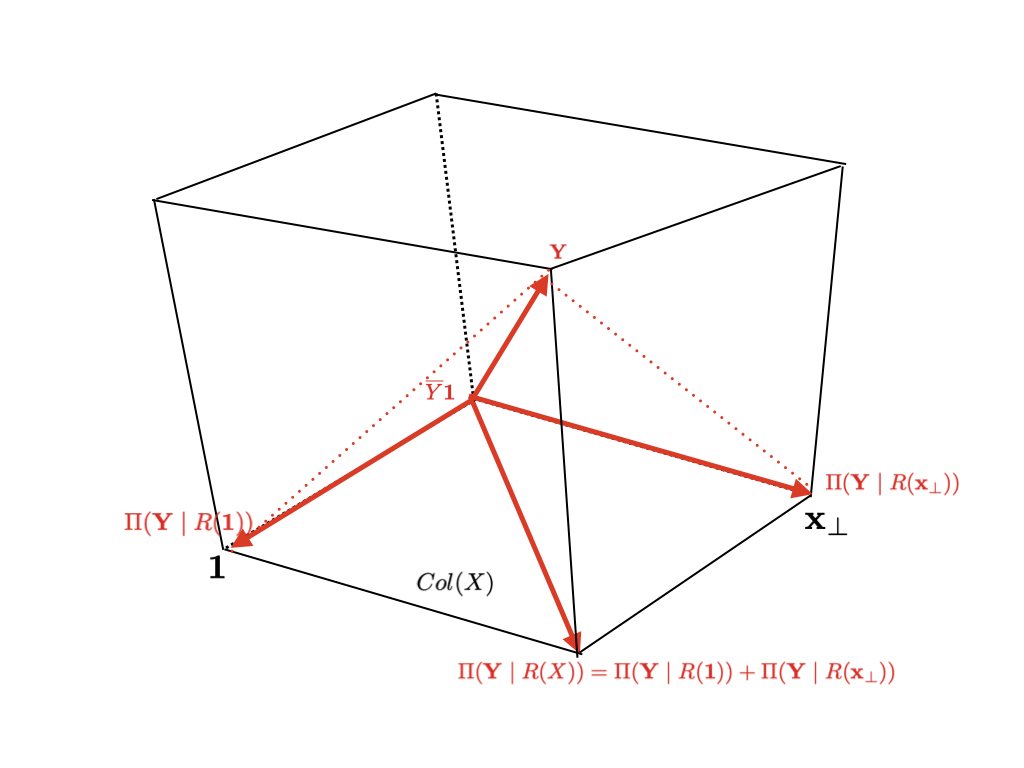
\includegraphics[width=0.7\linewidth]{images/multiple-qr1} 

}

\caption{Orthogonalized basis}\label{fig:qrpng}
\end{figure}

\begin{figure}[H]

{\centering 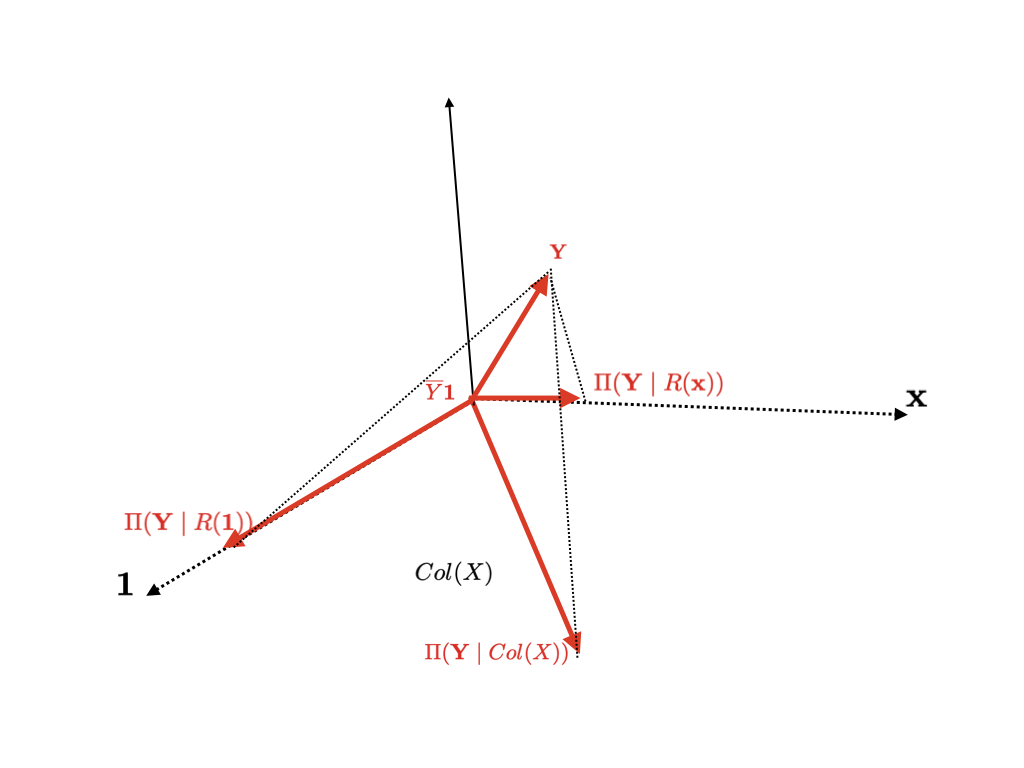
\includegraphics[width=0.7\linewidth]{images/multiple-qr2} 

}

\caption{Non-orthogonal basis}\label{fig:qrpng2}
\end{figure}

See Figure \ref{fig:qrpng}. By construbtion, projection onto each basis is same as \(\hat\beta_0\) and \(\hat\beta_1\). In Figure \ref{fig:qrpng2}, however, each projection is not regression coefficient.

\begin{figure}[H]

{\centering 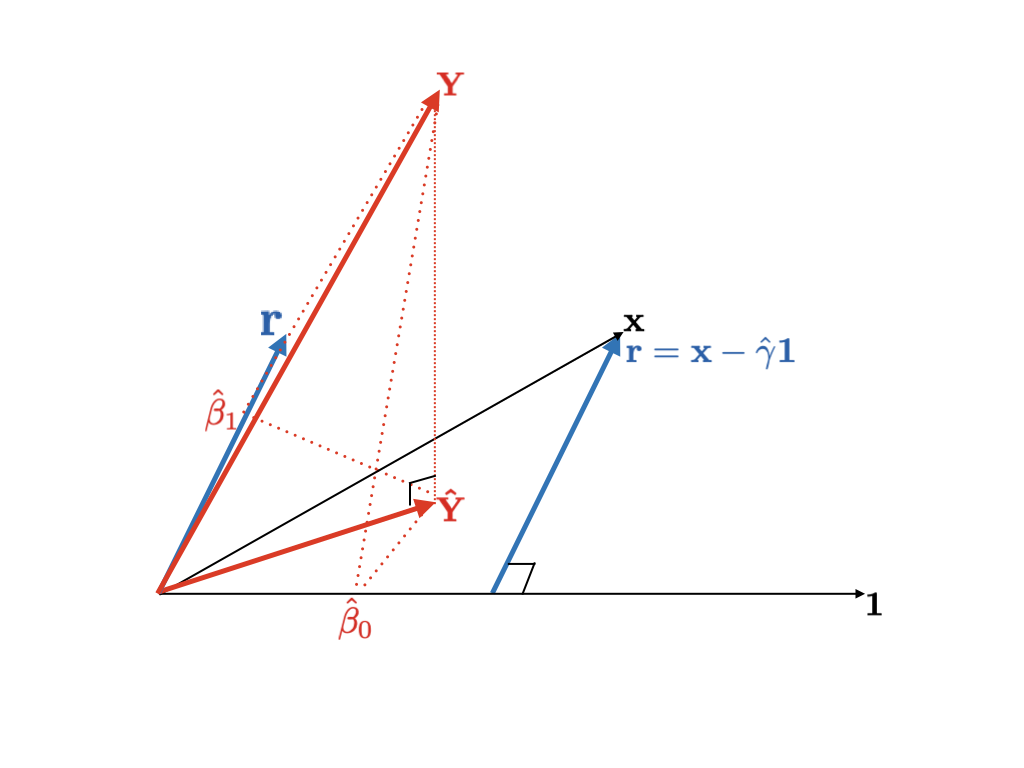
\includegraphics[width=0.7\linewidth]{images/multiple-qr3} 

}

\caption{QR decomposition for model matrix}\label{fig:simpledraw3}
\end{figure}

Regress \(\mathbf{x}\) onto \(\mathbf{1}\). Its residual can be a new orthogonalized predictor.

\hypertarget{properties-of-lse}{%
\subsection{Properties of LSE}\label{properties-of-lse}}

We have seen how we extend point estimator \(\boldsymbol{\hat\beta}\). In turn, we can check this is unbiased, and BLUE.

\BeginKnitrBlock{proposition}[Expectation and Variance]
\protect\hypertarget{prp:multbmoment}{}{\label{prp:multbmoment} \iffalse (Expectation and Variance) \fi{} }\(\boldsymbol{\hat\beta}\) is unbiased.

\begin{enumerate}
  \item $E\boldsymbol{\hat\beta} = \boldsymbol\beta$
  \item $Var\boldsymbol{\hat\beta} = \sigma^2(X^TX)^{-1}$
\end{enumerate}
\EndKnitrBlock{proposition}

\BeginKnitrBlock{proof}
\iffalse{} {Proof. } \fi{}\begin{equation*}
  \begin{split}
    E\boldsymbol{\hat\beta} & = E\bigg( (X^TX)^{-1}X^T\mathbf{Y} \bigg) \\
    & = (X^TX)^{-1}X^T E\mathbf{Y} \\
    & = (X^TX)^{-1}X^T X\boldsymbol\beta \\
    & = \boldsymbol\beta
  \end{split}
\end{equation*}

Hence, \(\boldsymbol{\hat\beta}\) is unbiased.

\begin{equation*}
  \begin{split}
    Var\boldsymbol{\hat\beta} & = Var\bigg( (X^TX)^{-1}X^T\mathbf{Y} \bigg) \\
    & = (X^TX)^{-1}X^T Var(\mathbf{Y}) X(X^TX)^{-1} \\
    & = (X^TX)^{-1}X^T(\sigma^2 I)X(X^TX)^{-1} \\
    & = \sigma^2 (X^TX)^{-1}
  \end{split}
\end{equation*}
\EndKnitrBlock{proof}

Since the variance of LSE have been revealed, now we want to know if this is the lowest one among estimators. Gauss-Markov theorem states that LSE has the lowest variance among linear unbiased estimators for \(\boldsymbol\beta\), so called the \textbf{best linear unbiased estimator (BLUE)}.

\BeginKnitrBlock{theorem}[Gauss-Markov Theorem]
\protect\hypertarget{thm:multgm}{}{\label{thm:multgm} \iffalse (Gauss-Markov Theorem) \fi{} }\(\boldsymbol{\hat\beta} = (X^TX)^{-1}X^T\mathbf{Y}\) is BLUE, i.e.

For any \(\tilde{\boldsymbol\beta} \in \Omega \equiv \{ \tilde{\boldsymbol\beta} : \tilde{\boldsymbol\beta} = C\mathbf{Y} , E\tilde{\boldsymbol\beta} = \boldsymbol\beta \}\),

\[Var(\boldsymbol{\hat\beta}) \le Var(\tilde{\boldsymbol\beta})\]
\EndKnitrBlock{theorem}

\BeginKnitrBlock{proof}
\iffalse{} {Proof. } \fi{}Let \(\tilde{\boldsymbol\beta} \in \Omega \equiv \{ \tilde{\boldsymbol\beta} : \tilde{\boldsymbol\beta} = C\mathbf{Y} , E\tilde{\boldsymbol\beta} = \boldsymbol\beta \}\)

Claim: \(Var(\tilde{\boldsymbol\beta}) - Var(\boldsymbol{\hat\beta})\) is non-negative definite.

Note that \(\boldsymbol{\hat\beta}\) is the one with \(C = (X^TX)^{-1}X^T\).

Set \(D := C - (X^TX)^{-1}X^T\). From unbiasedness,

\begin{equation*}
  \begin{split}
    E\tilde{\boldsymbol\beta} & = CE\mathbf{Y} \\
    & = CX\boldsymbol\beta \\
    & = \Big( (X^TX)^{-1}X^T + D \Big)X\boldsymbol\beta \\
    & = \boldsymbol\beta + DX\boldsymbol\beta \\
    & = \boldsymbol\beta
  \end{split}
\end{equation*}

Since \(\forall \boldsymbol\beta \in \mathbb{R}^{p + 1} : DX \boldsymbol\beta = \mathbf{0}\),

\begin{equation} \label{eq:prgm}
  DX = 0
\end{equation}

\begin{equation*}
  \begin{split}
    Var\tilde{\boldsymbol\beta} & = Var(C\mathbf{Y}) \\
    & = \sigma^2CC^T \\
    & = \sigma^2\Big( (X^TX)^{-1}X^T + D \Big) \Big( (X^TX)^{-1}X^T + D \Big)^T \\
    & = \sigma^2\Big( (X^TX)^{-1} + DX(X^TX)^{-1} + (X^TX)^{-1}X^TD^T + DD^T \Big) \\
    & = \sigma^2\Big( (X^TX)^{-1} + DD^T \Big) \qquad \because \eqref{eq:prgm} \\
    & = Var\boldsymbol{\hat\beta} + \sigma^2DD^T
  \end{split}
\end{equation*}

Note that \(DD^T\) is non-negative definite. Hence,

\[Var\tilde{\boldsymbol\beta} - Var\boldsymbol{\hat\beta} = \sigma^2DD^T\]

is non-negative definite. This completes the proof.
\EndKnitrBlock{proof}

As in simple linear regression setting, we define \emph{residuals} and explain \(\sigma^2\).

\BeginKnitrBlock{definition}[Residuals]
\protect\hypertarget{def:multres}{}{\label{def:multres} \iffalse (Residuals) \fi{} }Let \(\hat{\mathbf{Y}} = (\hat{Y_1}, \ldots, \hat{Y_n})^T\) with \(\hat{Y_i} = \hat\beta_0 + \hat\beta_1 x_{i1} + \cdots + \hat\beta_px_{ip}\). Then the residual is defined by

\[\mathbf{e} := (\ldots,Y_i - \hat\beta_0 - \hat\beta_1 x_{i1} - \cdots - \hat\beta_px_{ip}, \ldots)^T = \mathbf{Y} - \hat{\mathbf{Y}} \in \mathbb{R}^n\]
\EndKnitrBlock{definition}

Extending the simple setting, we estimate \(\sigma^2\) with inner product of residuals divided by its degrees of freedom, i.e.~\emph{MSE}. The degrees of freedom becomes \(n - \text{the number of coefficients}\). Thus, \(n - (p + 1) = n - p - 1\).

\BeginKnitrBlock{proposition}[Estimation of $\sigma^2$]
\protect\hypertarget{prp:multsigma}{}{\label{prp:multsigma} \iffalse (Estimation of \(\sigma^2\)) \fi{} }Let \(\mathbf{e} = \mathbf{Y} - \hat{\mathbf{Y}}\) be residuals as in Definition \ref{def:multres}. Then

\[\hat\sigma^2 = \frac{\lVert \mathbf{e} \rVert}{n - p - 1}\]
\EndKnitrBlock{proposition}

The reason we divide with degrees of freedom is to make \(\hat\sigma^2\) unbiased.

\BeginKnitrBlock{proposition}[Mean of $\hat\sigma^2$]
\protect\hypertarget{prp:multsigmean}{}{\label{prp:multsigmean} \iffalse (Mean of \(\hat\sigma^2\)) \fi{} }\(\hat\sigma^2\) is unbiased, i.e.

\[E\bigg( \lVert \mathbf{Y} - \hat{\mathbf{Y}} \rVert^2 \bigg) = (n - p - 1)\sigma^2\]
\EndKnitrBlock{proposition}

\BeginKnitrBlock{proof}
\iffalse{} {Proof. } \fi{}Since \(\mathbf{Y} = \Pi_X\mathbf{Y}\),

\begin{equation*}
  \begin{split}
    \lVert \mathbf{Y} - \hat{\mathbf{Y}} \rVert^2 & = \lVert (I - \Pi_X)\mathbf{Y} \rVert^2 \\
    & = \mathbf{Y}^T(I - \Pi_X)^T(I - \Pi_X)\mathbf{Y} \\
    & = \mathbf{Y}^T (I - \Pi_X)\mathbf{Y} \qquad \because (I - \Pi_X): \text{symmetric idempotent}
  \end{split}
\end{equation*}

Since \(\mathbf{Y}^T (I - \Pi_X)\mathbf{Y} \in \mathbb{R}\),

\begin{equation*}
  \begin{split}
    \mathbf{Y}^T (I - \Pi_X)\mathbf{Y} & = tr\bigg( \mathbf{Y}^T (I - \Pi_X)\mathbf{Y} \bigg) \\
    & = tr\bigg( (I - \Pi_X)\mathbf{Y} \mathbf{Y}^T \bigg)
  \end{split}
\end{equation*}

Then

\begin{equation*}
  \begin{split}
    E\lVert \mathbf{Y} - \hat{\mathbf{Y}} \rVert^2 & = E\Big[ \mathbf{Y}^T (I - \Pi_X)\mathbf{Y} \Big] \\
    & = E\bigg[ tr\Big( (I - \Pi_X)\mathbf{Y} \mathbf{Y}^T \Big) \bigg] \\
    & = tr\bigg( (I - \Pi_X) \underset{(\ast)}{\underline{E\Big[ \mathbf{Y} \mathbf{Y}^T \Big]}} \bigg)
  \end{split}
\end{equation*}

Consider \((\ast)\).

\begin{equation*}
  \begin{split}
    E(\mathbf{Y}\mathbf{Y}^T) & = Var\mathbf{Y} + (E\mathbf{Y})(E\mathbf{Y})^T \\
    & = \sigma^2 I + X\boldsymbol\beta\boldsymbol\beta^T X^T
  \end{split}
\end{equation*}

Hence,

\begin{equation*}
  \begin{split}
    E\lVert \mathbf{Y} - \hat{\mathbf{Y}} \rVert^2 & = tr\bigg( (I - \Pi_X) E\Big[ \mathbf{Y} \mathbf{Y}^T \Big] \bigg) \\
    & = tr\bigg((I - \Pi_X)\sigma^2 + (I - \Pi_X)X\boldsymbol\beta\boldsymbol\beta^T X^T \bigg) \\
    & = tr\bigg( (I - \Pi_X)\sigma^2 \bigg) + tr\bigg( \boldsymbol\beta^T X^T(I - \Pi_X)X\boldsymbol\beta \bigg) \qquad \because (I - \Pi_X)X\boldsymbol\beta = X\boldsymbol\beta - X\boldsymbol\beta = 0 \\
    & = tr\bigg( (I - \Pi_X)\sigma^2 \bigg) \\
    & = (n - p - 1)\sigma^2 \qquad \because \begin{cases} tr(I) = n \\ tr(\Pi_X) = p + 1 \end{cases}
  \end{split}
\end{equation*}
\EndKnitrBlock{proof}

In this proposition, we have used model matrix directly. Instead, we can use Equation \eqref{eq:qrhat} for simplicity.

\BeginKnitrBlock{proposition}[Variance using QR decomposition]
\protect\hypertarget{prp:qrmoment}{}{\label{prp:qrmoment} \iffalse (Variance using QR decomposition) \fi{} }Let \(X = QR\). Then \(\boldsymbol{\hat\beta} = R^{-1}Q^T\mathbf{Y}\). It follows that

\[Var\boldsymbol{\hat\beta} = \sigma^2(R^TR)^{-1}\]
\EndKnitrBlock{proposition}

\BeginKnitrBlock{proof}
\iffalse{} {Proof. } \fi{}It proceeds in a similar way for \(\boldsymbol{\hat\beta} = R^{-1}Q^T\mathbf{Y}\).

\begin{equation*}
  \begin{split}
    Var\boldsymbol{\hat\beta} & = Var\bigg( R^{-1}Q^T\mathbf{Y} \bigg) \\
    & = R^{-1}Q^T Var(\mathbf{Y}) Q(R^T)^{-1} \\
    & = R^{-1}Q^T (\sigma^2 I) Q(R^T)^{-1} \\
    & = \sigma^2 (R^TR)^{-1} \qquad \because Q^TQ = I \\
  \end{split}
\end{equation*}
\EndKnitrBlock{proof}

\BeginKnitrBlock{proposition}[QR representation for residual]
\protect\hypertarget{prp:qrres}{}{\label{prp:qrres} \iffalse (QR representation for residual) \fi{} }Let \(X = QR\). Then

\[\mathbf{e} = (I - QQ^T)\mathbf{Y}\]
\EndKnitrBlock{proposition}

\BeginKnitrBlock{proof}
\iffalse{} {Proof. } \fi{}From Equation \eqref{eq:qrfit},

\[\Pi_X = QQ^T\]

Hence,

\[\mathbf{e} = (I - \Pi_X)\mathbf{Y} = (I - QQ^T)\mathbf{Y}\]
\EndKnitrBlock{proof}

On Figure \ref{fig:simpledraw3}, we can see these relations. Operation \(Q^T\mathbf{Y}\) is just projection to each orthogonal basis. \(Q\) sums these projection so that we get \(\mathbf{\hat{Y}}\) which projection of \(\mathbf{Y}\) onto the column space of model matrix.

\begin{figure}[H]

{\centering 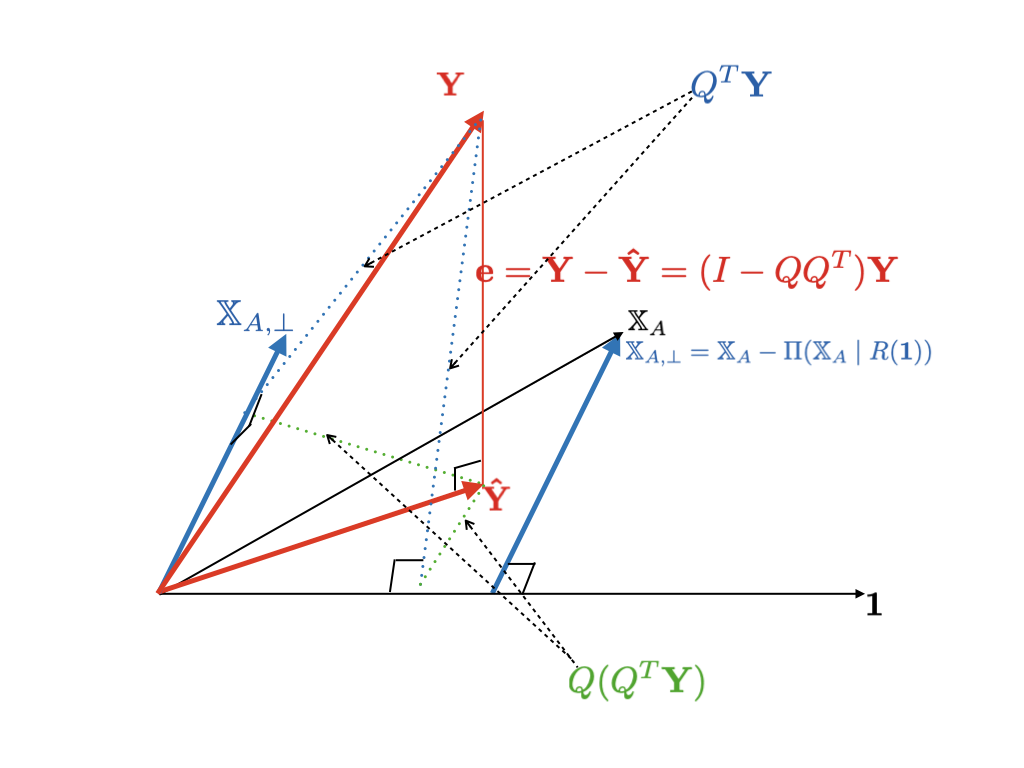
\includegraphics[width=0.7\linewidth]{images/multiple-residual} 

}

\caption{Residual vector}\label{fig:multresfig}
\end{figure}

\hypertarget{mean-response-and-response-1}{%
\subsection{Mean response and response}\label{mean-response-and-response-1}}

Let \(\mathbf{z} = (z_1, \ldots, z_p)^T\).

\BeginKnitrBlock{theorem}[Estimation of the mean response]
\protect\hypertarget{thm:multmeanres}{}{\label{thm:multmeanres} \iffalse (Estimation of the mean response) \fi{} }\[\hat\mu_z = \hat\beta_0 + \mathbf{z}^T\boldsymbol{\hat\beta}_A\]
\EndKnitrBlock{theorem}

\BeginKnitrBlock{theorem}[(out of sample) Prediction of a response]
\protect\hypertarget{thm:multpred}{}{\label{thm:multpred} \iffalse ((out of sample) Prediction of a response) \fi{} }\[\hat{Y}_z = \hat\beta_0 + \mathbf{z}^T \boldsymbol{\hat\beta}_Z\]
\EndKnitrBlock{theorem}

\BeginKnitrBlock{proposition}[Residual vector]
\protect\hypertarget{prp:multresprop}{}{\label{prp:multresprop} \iffalse (Residual vector) \fi{} }Let \(\mathbf{e} = (I - \Pi_X)\mathbf{Y}\). Then

\begin{enumerate}
  \item $Var(\mathbf{e}) = \sigma^2(I - \Pi_X)$
  \item $\mathbf{e} \perp \mathbf{\hat{Y}}$
\end{enumerate}
\EndKnitrBlock{proposition}

\BeginKnitrBlock{proof}[$Var(\mathbf{e})$]
\iffalse{} {Proof (\(Var(\mathbf{e})\)). } \fi{}\begin{equation*}
  \begin{split}
    Var(\mathbf{e}) & = Var\Big( (I - \Pi_X)\mathbf{Y} \Big) \\
    & = (I - \Pi_X) Var(\mathbf{Y}) (I - \Pi_X)^T \\
    & = \sigma^2 (I - \Pi_X) \qquad \because (I - \Pi_X) \:\text{symmetric itempotent}
  \end{split}
\end{equation*}
\EndKnitrBlock{proof}

\BeginKnitrBlock{proof}[$\mathbf{e} \perp \mathbf{\hat{Y}}$]
\iffalse{} {Proof (\(\mathbf{e} \perp \mathbf{\hat{Y}}\)). } \fi{}Note that

\[\mathbf{e} \in Col(X)^{\perp}\]

From the properties of projection, we have

\begin{equation}
  \begin{cases}
    \mathbf{e} \perp \mathbf{1} \\
    \mathbf{e} \perp \mathbf{x}_j & \forall j = 1, 2, \ldots, p
  \end{cases}
  \label{eq:multnormaleq}
\end{equation}

Since \(\hat{Y_i} = \hat\beta_0 + \hat\beta_1 x_{i1} + \cdots + \hat\beta_p x_{ip}\),

\[\mathbf{e} \perp \mathbf{\hat{Y}}\]
\EndKnitrBlock{proof}

Equation \eqref{eq:multnormaleq} is another form of the \emph{normal equation}.

\BeginKnitrBlock{remark}
\iffalse{} {Remark. } \fi{}The least squares regression line \(\{ (\mathbf{z}, y) : y = \hat\beta_0 + \mathbf{z}^T\hat\beta_A \}\) always passes through

\[\bigg( \frac{1}{n} \mathbb{X}_A^T \mathbf{1}, \overline{Y} \bigg)\]

In simple linear regression setting,

\[(\overline{x}, \overline{Y})\]
\EndKnitrBlock{remark}

\BeginKnitrBlock{proof}
\iffalse{} {Proof. } \fi{}First consider \(p = 1\). Normal equation gives directly that

\[\hat\beta_0 = \overline{Y} - \hat\beta_1 \overline{x}\]

Thus,

\[\overline{Y} = \hat\beta_0 + \hat\beta_1 \overline{x}\]

We now give more general proof, i.e.~for \(p \ge 1\).

Claim: \(\overline{Y} = \hat\beta_0 + \bigg(\frac{1}{n} \mathbb{X}_A^T \mathbf{1} \bigg)^T \boldsymbol{\hat\beta}_A\)

From Equation \eqref{eq:orthbeta},

\[\hat\beta_0 = \overline{Y} - \frac{1}{n}\mathbf{1}^T\mathbb{X}_A\boldsymbol{\hat\beta}_A\]

It follows that

\[\overline{Y} = \hat\beta_0 + \frac{1}{n}\mathbf{1}^T\mathbb{X}_A\boldsymbol{\hat\beta}_A\]

This completes the proof.
\EndKnitrBlock{proof}

\hypertarget{analysis-of-variance-1}{%
\section{Analysis of Variance}\label{analysis-of-variance-1}}

\hypertarget{decomposition-of-sst}{%
\subsection{Decomposition of SST}\label{decomposition-of-sst}}

We have

\begin{itemize}
\tightlist
\item
  \(SST = \lVert \mathbf{Y} - \overline{Y}\mathbf{1} \rVert^2 = \mathbf{Y}^T(I - \Pi_{\mathbf{1}})\mathbf{Y}\)
\item
  \(SSR = \lVert \mathbf{\hat{Y}} - \overline{Y}\mathbf{1} \rVert^2 = \mathbf{Y}^T(\Pi_X - \Pi_{\mathbf{1}})\mathbf{Y}\)
\item
  \(SSE = \lVert \mathbf{Y} - \mathbf{\hat{Y}} \rVert^2 = \mathbf{Y}^T(I - \Pi_X)\mathbf{Y}\)
\end{itemize}

\begin{figure}[H]

{\centering 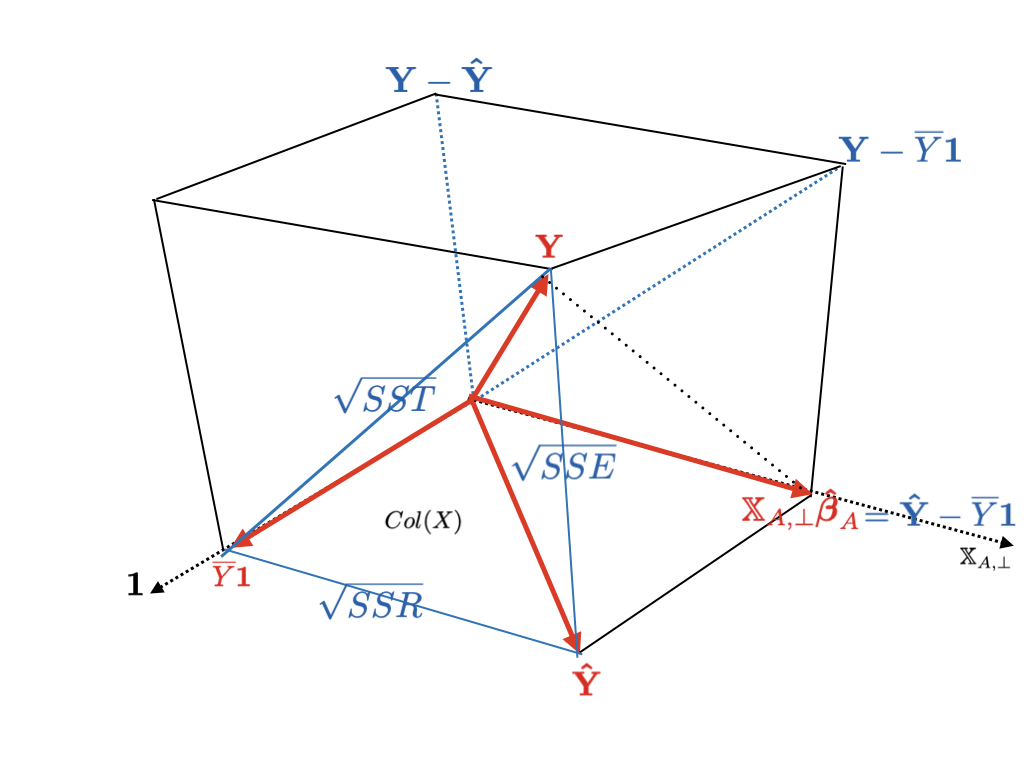
\includegraphics[width=0.7\linewidth]{images/multiple-anova} 

}

\caption{Decomposition of SST}\label{fig:mdecomp}
\end{figure}

In Figure \ref{fig:mdecomp}, Pythagorean law gives

\[SST = SSR + SSE\]

\BeginKnitrBlock{lemma}
\protect\hypertarget{lem:unnamed-chunk-71}{}{\label{lem:unnamed-chunk-71} }Let \(X = [\mathbf{1} \mid \mathbb{X}_A]\) and let \(\mathbb{X}_{A, \perp} = \mathbb{X}_A - \Pi_{\mathbf{1}}\mathbb{X}_A\). Then

\[\mathbf{\hat{Y}} - \overline{Y}\mathbf{1} = \mathbb{X}_{A, \perp}\boldsymbol{\hat\beta}_A\]
\EndKnitrBlock{lemma}

\BeginKnitrBlock{proof}
\iffalse{} {Proof. } \fi{}Note that \(\mathbf{1} \perp \mathbb{X}_{A, \perp}\).

Recall that

\[\Pi(\mathbf{Y} \mid R(\mathbf{1})) = \mathbf{1}(\mathbf{1}^T\mathbf{1})^{-1}\mathbf{1}^T\mathbf{Y} = \overline{Y}\mathbf{1}\]

From Theorem \ref{thm:orthdecomp},

\begin{equation*}
  \begin{split}
    \mathbf{\hat{Y}} & = \Pi(\mathbf{Y} \mid R(\mathbf{1})) + \Pi(\mathbf{Y} \mid R(\mathbb{X}_{A,\perp})) \\
    & = \overline{Y}\mathbf{1} + \mathbb{X}_{A,\perp}\boldsymbol{\hat\beta}_A
  \end{split}
\end{equation*}

Hence,

\[\mathbf{\hat{Y}} - \overline{Y}\mathbf{1} = \mathbb{X}_{A,\perp}\boldsymbol{\hat\beta}_A\]
\EndKnitrBlock{proof}

\hypertarget{distributions}{%
\subsection{Distributions}\label{distributions}}

\BeginKnitrBlock{proposition}[Distribution of SS]
\protect\hypertarget{prp:ssdist}{}{\label{prp:ssdist} \iffalse (Distribution of SS) \fi{} }Extending for \(p > 1\), we can get each result.

\begin{enumerate}
  \item $\frac{SSE}{\sigma^2} \sim \chi^2(n - p - 1)$
  \item $\frac{SSR}{\sigma^2} \sim \chi^2(p, \delta), \quad \delta = \frac{\boldsymbol\beta^TX^T(\Pi_X - \Pi_{\mathbf{1}})X\boldsymbol\beta}{\sigma^2}$
  \item $SSR \perp\!\!\!\perp SSE$
  \item $SSE \perp\!\!\!\perp\boldsymbol{\hat\beta}$
  \item $\frac{SST}{\sigma^2} \sim \chi^2(n - 1, \delta), \quad \delta = \frac{\boldsymbol\beta^TX^T(I - \Pi_{\mathbf{1}})X\boldsymbol\beta}{\sigma^2}$
\end{enumerate}
\EndKnitrBlock{proposition}

\BeginKnitrBlock{proof}[Distribution of SSE]
\iffalse{} {Proof (Distribution of SSE). } \fi{}Note that

\[SSE = \mathbf{Y}^T(I - \Pi_X)\mathbf{Y}\]

From Theorem \ref{thm:quaddist},

\[K = rank(I - \Pi_X) = tr(I - \Pi_X) = n - rank(\Pi_X) = n - p - 1\]

\(\delta\) proof is exactly same as Proposition \ref{prp:ssedist}.

\begin{equation*}
  \begin{split}
    \delta & = \bigg(\frac{X\boldsymbol\beta}{\sigma}\bigg)^T (I - \Pi_X) \bigg(\frac{X\boldsymbol\beta}{\sigma}\bigg) \\
    & = \frac{\boldsymbol\beta^TX^TX\boldsymbol\beta}{\sigma^2} - \frac{(\boldsymbol\beta^TX^T)X(X^TX)^{-1}X^T(X\boldsymbol\beta)}{\sigma^2} \\
    & = \frac{\boldsymbol\beta^TX^TX\boldsymbol\beta}{\sigma^2} - \frac{\boldsymbol\beta^TX^TX\boldsymbol\beta}{\sigma^2} \\
    & = 0
  \end{split}
\end{equation*}

Hence, \(\delta = 0\).
\EndKnitrBlock{proof}

\BeginKnitrBlock{proof}[Distribution of SSR]
\iffalse{} {Proof (Distribution of SSR). } \fi{}Note that

\[SSR = \mathbf{Y}^T(\Pi_X - \Pi_{\mathbf{1}})\mathbf{Y}\]

From Theorem \ref{thm:quaddist},

\[K = rank(\Pi_X - \Pi_{\mathbf{1}}) = tr(\Pi_X) - tr(\Pi_{\mathbf{1}}) = rank(\Pi_X) - rank(\Pi_{\mathbf{1}}) = p + 1 - 1 = p\]

\(\delta\) proof is exactly same as Proposition \ref{prp:ssrdist}.

\begin{equation}
  \begin{split}
    \delta & = \bigg(\frac{X\boldsymbol\beta}{\sigma}\bigg)^T (\Pi_X - \Pi_{\mathbf{1}}) \bigg(\frac{X\boldsymbol\beta}{\sigma}\bigg) \qquad \because \frac{\mathbf{Y}}{\sigma} \sim MVN(\frac{1}{\sigma}X\boldsymbol\beta, I) \\
    & = \frac{\boldsymbol\beta^T \Big\{ X^T(\Pi_X - \Pi_{\mathbf{1}})X \Big\} \boldsymbol\beta }{\sigma^2}
  \end{split}
  \label{eq:multssrdel}
\end{equation}

This completes the proof.
\EndKnitrBlock{proof}

In univariate setting, we have seen that \(\delta\) is expressed in terms of \(\hat\beta_1\) excluding \(\hat\beta_0\). How about in multivariate? In Equation \eqref{eq:multssrdel}, we can block design matrix \(X\) into

\[X = \begin{bmatrix} \mathbf{1} \mid \mathbb{X}_A \end{bmatrix}\]

One proceeds in a similar way. Since both \(\mathbf{1}, \mathbb{X}_A \in Col(X)\),

\[\Pi_X \mathbf{1} = \mathbf{1}, \qquad \Pi_X \mathbb{X}_A = \mathbb{X}_A\]

Since \(\mathbf{1} \in R(\{ \mathbf{1} \})\),

\[\Pi_{\mathbf{1}} \mathbf{1} = \mathbf{1}\]

Since \(\Pi_{\mathbf{1}} = \frac{1}{n}\mathbf{1}\mathbf{1}^T\),

\[
\Pi_{\mathbf{1}}\mathbb{X}_A = \mathbf{1} \mathbf{\overline{x}}^T = \begin{bmatrix}
  \overline{x}_1 & \overline{x}_2 & \cdots & \overline{x}_p \\
  \overline{x}_1 & \overline{x}_2 & \cdots & \overline{x}_p \\
  \vdots & \vdots & \vdots & \vdots \\
  \overline{x}_1 & \overline{x}_2 & \cdots & \overline{x}_p
\end{bmatrix}
\]

Using these facts, we have following

\begin{equation} \label{eq:mssrquad1}
  \mathbf{1}^T (\Pi_X - \Pi_{\mathbf{1}}) \mathbf{1} = \mathbf{1}^T (\mathbf{1} - \mathbf{1}) = 0
\end{equation}

\begin{equation} \label{eq:mssrquad2}
  \begin{split}
    \mathbf{1}^T (\Pi_X - \Pi_{\mathbf{1}}) \mathbb{X}_A & = \mathbf{1}^T (\mathbb{X}_A - \mathbf{1} \mathbf{\overline{x}}^T) \\
    & = \mathbf{1}^T \begin{bmatrix}
      x_{ij} - \overline{x}_j
    \end{bmatrix}_{1 \times j} \\
    & = \begin{bmatrix}
      \sum_i x_{ij} - n \overline{x}_j
    \end{bmatrix}_{1 \times j} \\
    & 0
  \end{split}
\end{equation}

\begin{equation} \label{eq:mssrquad3}
  \mathbb{X}_A^T (\Pi_X - \Pi_{\mathbf{1}}) \mathbf{1} = \mathbb{X}_A^T (\mathbf{1} - \mathbf{1}) = 0
\end{equation}

From Lemma \ref{lem:sxy},

\begin{equation} \label{eq:mssrquad4}
  \begin{split}
    \mathbb{X}_A^T (\Pi_X - \Pi_{\mathbf{1}}) \mathbb{X}_A & = \mathbb{X}_A^T \begin{bmatrix}
      x_{ij} - \overline{x}_j
    \end{bmatrix}_{1 \times j} \\
    & = \begin{bmatrix}
      \sum_i x_{ij}(x_{jk} - \overline{x}_k)
    \end{bmatrix}_{j \times k} \\
    & = \begin{bmatrix}
      \sum_i (x_{ij} - \overline{x}_j) (x_{ik} - \overline{x}_k)
    \end{bmatrix}_{j \times k} \\
    & = (n - 1) Var(\mathbb{X}_A) \\
    & \equiv S
  \end{split}
\end{equation}

Hence,

\begin{equation}
  \begin{split}
    \delta & = \frac{\boldsymbol\beta^T \Big\{ \begin{bmatrix} \mathbf{1} \mid \mathbb{X}_A \end{bmatrix}^T(\Pi_X - \Pi_{\mathbf{1}})\begin{bmatrix} \mathbf{1} \mid \mathbb{X}_A \end{bmatrix} \Big\} \boldsymbol\beta }{\sigma^2} \\
    & = \frac{\boldsymbol\beta^T \left[\begin{array}{c|c}
      \eqref{eq:mssrquad1} & \eqref{eq:mssrquad2} \\ \hline
      \eqref{eq:mssrquad3} & \eqref{eq:mssrquad4}
    \end{array}\right] \boldsymbol\beta}{\sigma^2} \\
    & = \frac{\boldsymbol\beta^T \left[\begin{array}{c|c}
      0 & 0 \\ \hline
      0 & S
    \end{array}\right] \boldsymbol\beta}{\sigma^2} \\
    & = \frac{\boldsymbol\beta_A^T S \boldsymbol\beta_A}{\sigma^2}
  \end{split}
  \label{eq:mssrdelta}
\end{equation}

\BeginKnitrBlock{proof}[Independence between SSE and SSR]
\iffalse{} {Proof (Independence between SSE and SSR). } \fi{}Since \(SSE\) and \(SSR\) are quadratic form of \(\mathbf{Y} \sim MVN(X\boldsymbol\beta, \sigma^2 I)\) and each \(I - \Pi_X\) and \(\Pi_X - \Pi_{\mathbf{1}}\) is symmetric,

Claim: \((I - \Pi_X)(\Pi_X - \Pi_{\mathbf{1}}) = 0\)

We have already shown this in Proposition \ref{prp:ssind}. Using the fact that \(\Pi_X\Pi_{\mathbf{1}} = \Pi_{\mathbf{1}}\),

\begin{equation*}
  \begin{split}
    (I - \Pi_X)(\Pi_X - \Pi_{\mathbf{1}}) & = \Pi_X - \Pi_{\mathbf{1}} - \Pi_X^2 + \Pi_X\Pi_{\mathbf{1}} \\
    & = \Pi_X - \Pi_{\mathbf{1}} - \Pi_X + \Pi_{\mathbf{1}} \qquad \because \text{idempotent} \\
    & = 0
  \end{split}
\end{equation*}
\EndKnitrBlock{proof}

\BeginKnitrBlock{proof}[Independence between SSE and regression vector]
\iffalse{} {Proof (Independence between SSE and regression vector). } \fi{}The proof is same as \ref{prp:ssbind}, by showing that \(((X^TX)^{-1}X^T)(I - \Pi_X) = 0\).

Since \(\Pi_X = X(X^TX)^{-1}X^T\),

\[((X^TX)^{-1}X^T)(I - \Pi_X) = (X^TX)^{-1}X^T - (X^TX)^{-1}X^T = 0\]

This completes the proof.
\EndKnitrBlock{proof}

\BeginKnitrBlock{proof}[Distribution of SST]
\iffalse{} {Proof (Distribution of SST). } \fi{}Note that

\[SST = \mathbf{Y}^T(I - \Pi_{\mathbf{1}})\mathbf{Y}\]

From Theorem \ref{thm:quaddist},

\[K = rank(I - \Pi_{\mathbf{1}}) = tr(I - \Pi_{\mathbf{1}}) = n - 1\]

and

\begin{equation*}
  \begin{split}
    \delta & = \bigg(\frac{X\boldsymbol\beta}{\sigma}\bigg)^T (I - \Pi_{\mathbf{1}}) \bigg(\frac{X\boldsymbol\beta}{\sigma}\bigg) \\
    & = \frac{\boldsymbol\beta^TX^T(I - \Pi_{\mathbf{1}})X\boldsymbol\beta}{\sigma^2}
  \end{split}
\end{equation*}
\EndKnitrBlock{proof}

\hypertarget{anova-for-testing-significance-of-regression-1}{%
\subsection{ANOVA for testing significance of regression}\label{anova-for-testing-significance-of-regression-1}}

Under the normality of error term

\[\boldsymbol\epsilon_i \sim MVN(\mathbf{0}, \sigma^2 I)\]

a test statistic can follow \(F\)-distribution as in univariate setting.

\BeginKnitrBlock{corollary}[F-test]
\protect\hypertarget{cor:ftest}{}{\label{cor:ftest} \iffalse (F-test) \fi{} }Under normality,

\[F = \frac{SSR / p}{SSE / (n - p - 1)} \sim F(p, n - p - 1, \delta)\]

where

\(\delta = \frac{\boldsymbol\beta^TX^T(\Pi_X - \Pi_{\mathbf{1}})X\boldsymbol\beta}{\sigma^2}\)
\EndKnitrBlock{corollary}

In the proof of \ref{prp:ssrdist}, we can understand the structure that \(\delta = 0\) when all coefficients corresponding to predictors are zero.

\[F \stackrel{H_0}{\sim} F(p, n - p - 1)\]

where

\[H_0: \beta_1 = \beta_2 = \cdots = \beta_p = 0\]

As other ordinary test, we just reject this \(H_0\) if observed \(F_0\) is large, i.e.

\[F_0 > F_{\alpha}(p, n - p - 1)\]

See Figure \ref{fig:goodfitfig}. \textbf{ANOVA table} summarizes these statistics in table form.

\begin{longtable}[]{@{}cccccc@{}}
\toprule
Source & SS & df & MS & F & p-value\tabularnewline
\midrule
\endhead
Model & \(SSR\) & \(p\) & \(MSR = \frac{SSR}{p}\) & \(F_0 = \frac{MSR}{MSE}\) & p-value\tabularnewline
Error & \(SSE\) & \(n - p - 1\) & \(MSE = \frac{SSE}{n - p - 1}\) & &\tabularnewline
Total & \(SST\) & \(n - 1\) & & &\tabularnewline
\bottomrule
\end{longtable}

Everything is same in \texttt{R}.

\begin{Shaded}
\begin{Highlighting}[]
\NormalTok{cem_fit <-}\StringTok{ }\KeywordTok{lm}\NormalTok{(y }\OperatorTok{~}\StringTok{ }\NormalTok{., }\DataTypeTok{data =}\NormalTok{ cem)}
\KeywordTok{summary}\NormalTok{(cem_fit)}
\CommentTok{#> }
\CommentTok{#> Call:}
\CommentTok{#> lm(formula = y ~ ., data = cem)}
\CommentTok{#> }
\CommentTok{#> Residuals:}
\CommentTok{#>    Min     1Q Median     3Q    Max }
\CommentTok{#> -3.175 -1.671  0.251  1.378  3.925 }
\CommentTok{#> }
\CommentTok{#> Coefficients:}
\CommentTok{#>             Estimate Std. Error t value Pr(>|t|)  }
\CommentTok{#> (Intercept)   62.405     70.071    0.89    0.399  }
\CommentTok{#> x1             1.551      0.745    2.08    0.071 .}
\CommentTok{#> x2             0.510      0.724    0.70    0.501  }
\CommentTok{#> x3             0.102      0.755    0.14    0.896  }
\CommentTok{#> x4            -0.144      0.709   -0.20    0.844  }
\CommentTok{#> ---}
\CommentTok{#> Signif. codes:  0 '***' 0.001 '**' 0.01 '*' 0.05 '.' 0.1 ' ' 1}
\CommentTok{#> }
\CommentTok{#> Residual standard error: 2.45 on 8 degrees of freedom}
\CommentTok{#> Multiple R-squared:  0.982,  Adjusted R-squared:  0.974 }
\CommentTok{#> F-statistic:  111 on 4 and 8 DF,  p-value: 4.76e-07}
\end{Highlighting}
\end{Shaded}

You can see \texttt{F-statistic} with degrees of freedom 4 8.

\begin{Shaded}
\begin{Highlighting}[]
\KeywordTok{summary}\NormalTok{(cem_fit)}\OperatorTok{$}\NormalTok{fstatistic}
\CommentTok{#> value numdf dendf }
\CommentTok{#>   111     4     8}
\end{Highlighting}
\end{Shaded}

However, \texttt{anova.lm()} gives a bit different format This is related to \emph{extra sum of squares}, which will be covered later.

\begin{Shaded}
\begin{Highlighting}[]
\KeywordTok{anova}\NormalTok{(cem_fit)}
\CommentTok{#> Analysis of Variance Table}
\CommentTok{#> }
\CommentTok{#> Response: y}
\CommentTok{#>           Df Sum Sq Mean Sq F value  Pr(>F)    }
\CommentTok{#> x1         1   1450    1450  242.37 2.9e-07 ***}
\CommentTok{#> x2         1   1208    1208  201.87 5.9e-07 ***}
\CommentTok{#> x3         1     10      10    1.64    0.24    }
\CommentTok{#> x4         1      0       0    0.04    0.84    }
\CommentTok{#> Residuals  8     48       6                    }
\CommentTok{#> ---}
\CommentTok{#> Signif. codes:  0 '***' 0.001 '**' 0.01 '*' 0.05 '.' 0.1 ' ' 1}
\end{Highlighting}
\end{Shaded}

\hypertarget{coefficient-of-determination-1}{%
\subsection{Coefficient of determination}\label{coefficient-of-determination-1}}

In univariate setting, coefficient of determination measures linear relationship based on the \(SST\) decomposition.

\[R^2 = \frac{SSR}{SST} = \hat\rho = \cos\theta\]

Moreover, it becomes to be same as sample correlation \(\hat\rho\) and angle between two vectors. In multivariate setting, we also define this kind of measure.

\BeginKnitrBlock{definition}[Coefficient of Determination]
\protect\hypertarget{def:mrsq}{}{\label{def:mrsq} \iffalse (Coefficient of Determination) \fi{} }For \(\mathbf{Y}_i = X\boldsymbol\beta+ \epsilon_i\),

\[R^2 := \max_{\boldsymbol\beta\in \mathbb{R}^{p + 1}} \hat\rho(\mathbf{Y}, X\boldsymbol\beta)\]

where \(\hat\rho\) means sample correlation.
\EndKnitrBlock{definition}

We have mentioned about \(R^2 = (\cos\theta)^2\) in simple linear regression. See Equation \eqref{eq:rsqcos}. Now we try to see detail of this relation. First, in \citet{Leon:2014aa}, you might see the relation of \(\cos\theta\) and inner product.

\BeginKnitrBlock{lemma}
\protect\hypertarget{lem:cosprod}{}{\label{lem:cosprod} }If \(\mathbf{x}, \mathbf{y} \in \mathbb{R}^n\) are two nonzero vectors and \(\theta\) is the angle between them, then

\[\mathbf{x}^T\mathbf{y} = \lVert \mathbf{x} \rVert \lVert \mathbf{y} \rVert \cos\theta\]
\EndKnitrBlock{lemma}

\begin{figure}[H]

{\centering 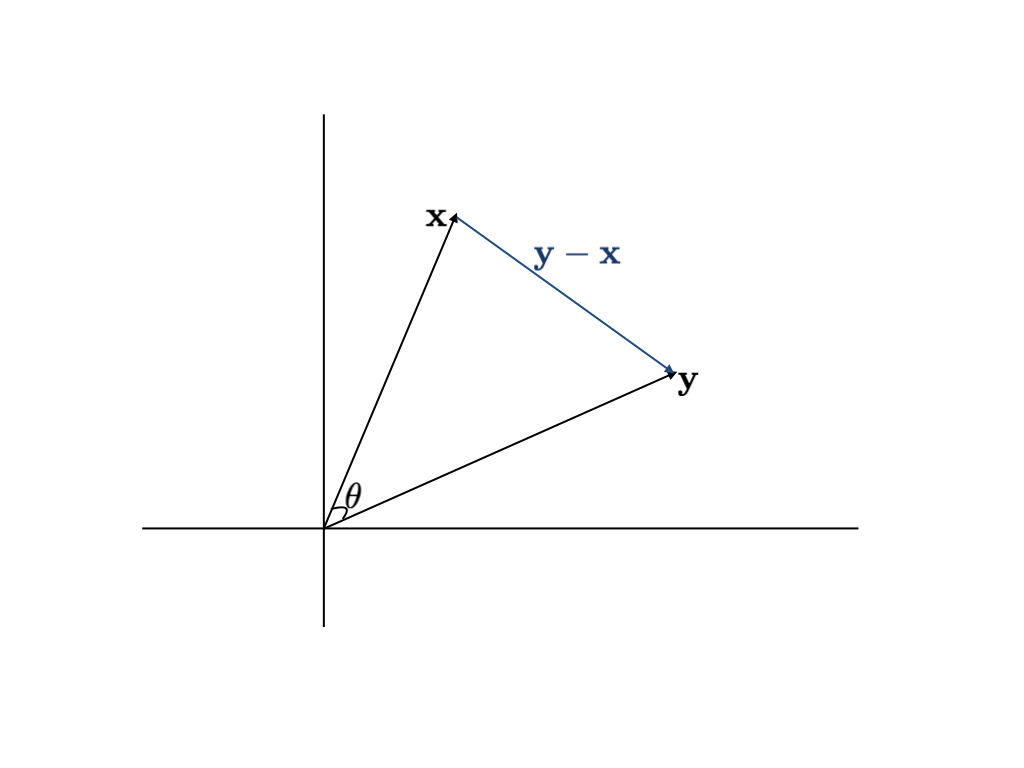
\includegraphics[width=0.7\linewidth]{images/multiple-cos} 

}

\caption{Two vectors in $\mathbb{R}^2$}\label{fig:cosfig}
\end{figure}

\BeginKnitrBlock{proof}
\iffalse{} {Proof. } \fi{}See Figure \ref{fig:cosfig}. We have a triangle. Law of cosines gives that

\[\lVert \mathbf{y} - \mathbf{x} \rVert^2 = \lVert \mathbf{x} \rVert^2 + \lVert \mathbf{y} \rVert^2 -2 \lVert \mathbf{x} \rVert \lVert \mathbf{y} \rVert \cos\theta\]

It follows that

\begin{equation*}
  \begin{split}
    \lVert \mathbf{x} \rVert \lVert \mathbf{y} \rVert \cos\theta & = \frac{1}{2}(\lVert \mathbf{x} \rVert^2 + \lVert \mathbf{y} \rVert^2 - \lVert \mathbf{y} - \mathbf{x} \rVert^2) \\
    & = \frac{1}{2}(\mathbf{x}^T \mathbf{x} + \mathbf{y}^T \mathbf{y} - (\mathbf{y} - \mathbf{x})^T(\mathbf{y} - \mathbf{x})) \\
    & = \mathbf{x}^T\mathbf{y}
  \end{split}
\end{equation*}
\EndKnitrBlock{proof}

This implies the \emph{relationship between sample correlation and the angle}.

\BeginKnitrBlock{theorem}[Sample correlation and the Angle]
\protect\hypertarget{thm:corrangle}{}{\label{thm:corrangle} \iffalse (Sample correlation and the Angle) \fi{} }Let \(\mathbf{X} = (X_1, \ldots, X_n)^T\) and \(\mathbf{Y} = (Y_1, \ldots, Y_n)^T\) be random variables. Then

\[\hat\rho(\mathbf{X}, \mathbf{Y}) = cos \theta\]

where \(\theta\) is the angle between \(\mathbf{X} - \overline{X}\mathbf{1}\) and \(\mathbf{Y} - \overline{Y}\mathbf{1}\).
\EndKnitrBlock{theorem}

\BeginKnitrBlock{proof}
\iffalse{} {Proof. } \fi{}Note that

\[\widehat{Cov}(\mathbf{X}, \mathbf{Y}) = \frac{1}{n - 1} (\mathbf{X} - \overline{X}\mathbf{1})^T(\mathbf{Y} - \overline{Y}\mathbf{1})\]

\[\hat\sigma_{\mathbf{X}} = \sqrt{\frac{1}{n - 1} (\mathbf{X} - \overline{X}\mathbf{1})^T (\mathbf{X} - \overline{X}\mathbf{1})}\]

and

\[\hat\sigma_{\mathbf{Y}} = \sqrt{\frac{1}{n - 1} (\mathbf{Y} - \overline{Y}\mathbf{1})^T (\mathbf{Y} - \overline{Y}\mathbf{1})}\]

and hence it follows that

\begin{equation*}
  \begin{split}
    \hat\rho(\mathbf{X}, \mathbf{Y}) & = \frac{\widehat{Cov}(\mathbf{X}, \mathbf{Y})}{\hat\sigma_{\mathbf{X}}\hat\sigma_{\mathbf{Y}}} \\
    & = \frac{(\mathbf{X} - \overline{X}\mathbf{1})^T(\mathbf{Y} - \overline{Y}\mathbf{1})}{\sqrt{(\mathbf{X} - \overline{X}\mathbf{1})^T (\mathbf{X} - \overline{X}\mathbf{1})}\sqrt{(\mathbf{Y} - \overline{Y}\mathbf{1})^T (\mathbf{Y} - \overline{Y}\mathbf{1})}} \\
    & = \frac{<\mathbf{X} - \overline{X}\mathbf{1}, \mathbf{Y} - \overline{Y}\mathbf{1}>}{\lVert \mathbf{X} - \overline{X}\mathbf{1} \rVert \lVert \mathbf{Y} - \overline{Y}\mathbf{1} \rVert} \\
    & = cos \theta
  \end{split}
\end{equation*}

where \(\theta\) is the angle between \(\mathbf{X} - \overline{X}\mathbf{1}\) and \(\mathbf{Y} - \overline{Y}\mathbf{1}\).
\EndKnitrBlock{proof}

Using this fact, we can finally derive that

\begin{equation}
  \hat\rho(\mathbf{Y}, X\boldsymbol\beta) = \cos\theta
  \label{eq:rsqangle}
\end{equation}

where \(\theta\) is the angle between \(\mathbf{Y} - \overline{Y}\mathbf{1}\) and

\[\beta_1(\mathbf{x}_1 - \overline{x}_1\mathbf{1}) + \cdots \beta_p(\mathbf{x}_p - \overline{x}_p\mathbf{1}) = \mathbb{X}_{A,\perp} \boldsymbol\beta_A \in Col(\mathbb{X}_{A, \perp})\]

\begin{figure}[H]

{\centering 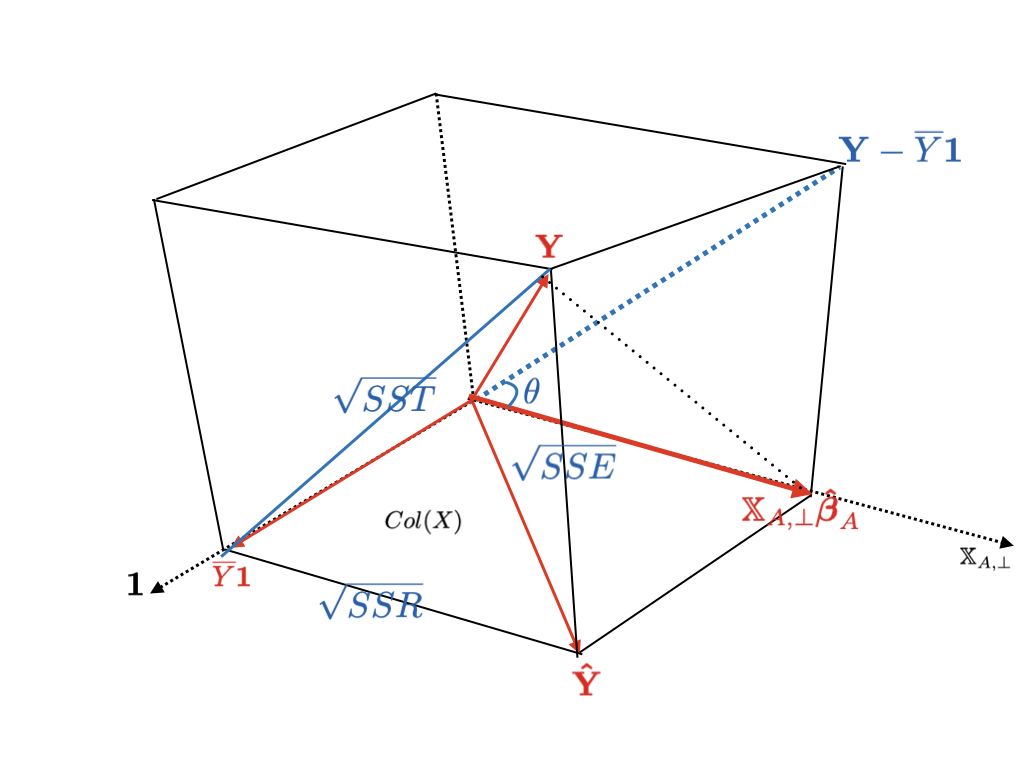
\includegraphics[width=0.7\linewidth]{images/multiple-rsq} 

}

\caption{$R^2$ and Projection}\label{fig:rsqfig}
\end{figure}

See Figure \ref{fig:rsqfig}. \(\theta\) is marked on Figure \ref{fig:mdecomp} setting. In this setting, we know that \(\theta < \frac{\pi}{2}\) is minimized by projection onto \(\mathbb{X}_{A,\perp}\). This means that \(\cos\theta\) is maximized. In other words,

\[R^2 = \frac{SSR}{SST} = (\cos\theta)^2\]

is maximized by the projection of \(\mathbf{Y} - \overline{Y}\mathbf{1}\) onto \(Col(\mathbb{X}_{A, \perp})\). Thus, \(R^2\) can be interpreted as \emph{proportion of variability of \(Y\) that is explained by the set of \(x_j\)s}. It is obvious that \(0 \le R^2 \le 1\).

\(R^2\) becomes larger if a set of \(\mathbb{X}_{A, \perp}\) explains the response well. Is it proper to use this measure as judging \emph{goodness-of-fit}? However, this is not a good measure for model comparison. Model comparison includes different number of predictors. \emph{\(SSE\), however, always decreases when new \(X_j\) is added,} while \(SST = \sum (Y_i - \overline{Y})\) never changes given \(Y\) data. This leads

\[R^2 = 1 - \frac{SSE}{SST}\]

always becomes larger by more predictors. For example,

\[
\begin{cases}
  Y = \beta_0 + \beta_1 X_1 + \epsilon \\
  Y = \beta_0 + \beta_1 X_1 + \beta_1 X_2 + \epsilon
\end{cases}
\]

Whether \(X_2\) additionaly contributes to \(Y\) significantly, \(R^2\) increases and we could judge that second model is better than first one. Hence to use this properly, we need some adjustment. As \(p + 1\) increases, this adjustment should become smaller:

\[\frac{n - 1}{n - p - 1}\]

\BeginKnitrBlock{definition}[Adjusted Rsquared]
\protect\hypertarget{def:ra}{}{\label{def:ra} \iffalse (Adjusted Rsquared) \fi{} }\[R_a^2 := 1 - \frac{SSE / (n - p - 1)}{SST / (n - 1)}\]
\EndKnitrBlock{definition}

\BeginKnitrBlock{remark}[Adjustment]
\iffalse{} {Remark (Adjustment). } \fi{}\[R_a^2 = 1 - \frac{n - 1}{n - p - 1}(1 - R^2)\]
\EndKnitrBlock{remark}

\BeginKnitrBlock{proof}
\iffalse{} {Proof. } \fi{}Note that

\[R^2 = 1 - \frac{SSE}{SST}\]

and hence,

\begin{equation*}
  \begin{split}
    R_a^2 & := 1 - \frac{SSE / (n - p - 1)}{SST / (n - 1)} \\
    & = 1 - \frac{n - 1}{n - p - 1}\bigg(\frac{SSE}{SST}\bigg) \\
    & = 1 - \frac{n - 1}{n - p - 1}(1 - R^2)
  \end{split}
\end{equation*}
\EndKnitrBlock{proof}

So \(R_a^2\) becomes a useful measure for the goodness-of-fit. On the contrary, \emph{it cannot be interpreted as the proportion of total variation in \(Y\) that is explained by \(X_1, \ldots, X_p\).}

\hypertarget{distributions-1}{%
\section{Distributions}\label{distributions-1}}

\hypertarget{individual-regression-coefficients}{%
\subsection{Individual Regression coefficients}\label{individual-regression-coefficients}}

Under Normality,

\[\mathbf{Y} \sim MVN(X\boldsymbol\beta, \sigma^2I)\]

Since \(\boldsymbol{\hat\beta}\) is an unbiased estimator, Proposition \ref{prp:multbmoment} implies that

\begin{equation}
  \boldsymbol{\hat\beta}\sim MVN\bigg( \boldsymbol\beta, \sigma^2(X^TX)^{-1} \bigg)
  \label{eq:hbdist}
\end{equation}

Let \(C \equiv (X^TX)^{-1}\). Then

\[
\begin{bmatrix}
  \hat\beta_0 \\ \hline
  \hat\beta_1 \\ \hline
  \vdots \\ \hline
  \hat\beta_p
\end{bmatrix} \sim MVN\Bigg( \begin{bmatrix}
  \beta_0 \\ \hline
  \beta_1 \\ \hline
  \vdots \\ \hline
  \beta_p
\end{bmatrix}, \sigma^2\begin{bmatrix}
  c_{00} & \cdots & \cdots \\ \hline
  \cdots & c_{11} & \cdots \\ \hline
  \vdots & \vdots & \vdots \\ \hline
  \cdots & \cdots & c_{pp}
\end{bmatrix} \Bigg)
\]

i.e.~Individual coefficient follows

\[\hat\beta_j \sim N(\beta_j, c_{jj}\sigma^2), \quad j = 0, 1, \ldots, p\]

where \(c_{jj}\) is \(j + 1\)th diagonal element of \(C = (X^TX)^{-1}\). Then

\begin{equation}
  \frac{\hat\beta_k - \beta_k}{\sigma\sqrt{c_{kk}}} \sim N(0, 1)
  \label{eq:bejzdist}
\end{equation}

From Proposition \ref{prp:ssdist},

\[\frac{SSE}{\sigma^2} \sim \chi^2(n - p - 1)\]

Since \(\hat\sigma^2 = \frac{SSE}{n - p - 1}\) and \(\hat\beta_k \perp\!\!\!\perp\hat\sigma^2\),

\begin{equation}
  \frac{\hat\beta_k - \beta_k}{\hat\sigma\sqrt{c_{kk}}} = \frac{(\hat\beta_k - \beta_k) / (\sigma\sqrt{c_{kk}}) \sim N(0, 1)}{\sqrt{\frac{SSE}{\sigma^2} / (n - p - 1) \sim \chi^2(n - p - 1)}} \sim t(n - p - 1), \quad k = 0, 1, \ldots, p
  \label{eq:bejtdist}
\end{equation}

\hypertarget{mean-response-1}{%
\subsection{Mean response}\label{mean-response-1}}

Consider prediction at \(\mathbf{z} = (1, z_1, \ldots, z_p)^T\)

Mean response targets

\[\hat\mu_{\mathbf{z}} = \mathbf{z}^T\boldsymbol{\hat\beta}\]

From Equation \eqref{eq:hbdist},

\[\hat\mu_{\mathbf{z}} \sim N(\mathbf{z}^T\boldsymbol\beta, \sigma^2\mathbf{z}^T(X^TX)^{-1}\mathbf{z})\]

Set

\begin{equation}
  C_{\mathbf{z}} := \mathbf{z}^T(X^TX)^{-1}\mathbf{z}
  \label{eq:predse}
\end{equation}

Then by standardization,

\begin{equation}
  \frac{\hat\mu_{\mathbf{z}} - \mu_{\mathbf{z}}}{\sqrt{C_{\mathbf{z}}\sigma^2}} \sim N(0, 1)
  \label{eq:meanreszdist}
\end{equation}

Hence,

\begin{equation}
  \frac{\hat\mu_{\mathbf{z}} - \mu_{\mathbf{z}}}{\sqrt{C_{\mathbf{z}}\hat\sigma^2}} \sim t(n - p - 1)
  \label{eq:meanrestdist}
\end{equation}

\hypertarget{response-1}{%
\subsection{Response}\label{response-1}}

Now we target \(\mathbf{Y}\) at \(\mathbf{z} = (1, z_1, \ldots, z_p)^T\) \emph{out-of-sample}. \(\boldsymbol\epsilon_{\mathbf{z}}\) at this point is independent of the data set.

Consider

\begin{equation}
  \hat{Y}_{\mathbf{z}} - Y_{\mathbf{z}} = \mathbf{z}^T(\boldsymbol{\hat\beta}- \boldsymbol\beta) + \epsilon_{\mathbf{z}}
  \label{eq:prerrz}
\end{equation}

As in Proposition \ref{prp:bepsmvn}, it can be proven that

\[
\begin{bmatrix}
  \boldsymbol{\hat\beta}- \boldsymbol\beta\\
  \epsilon_{\mathbf{z}}
\end{bmatrix} \sim MVN
\]

by showing marginal follows Normal and two are independent. First part - marginal follows normal distribution - has been already shown and assumed. Since these are Normal, it is enough to show covariance is zero.

\begin{equation*}
  \begin{split}
    Cov((\boldsymbol{\hat\beta}- \boldsymbol\beta), \epsilon_{\mathbf{z}}) & = Cov\Big( (X^TX)^{-1}X^T Y, \epsilon_{\mathbf{z}} \Big) \\
    & = (X^TX)^{-1}X^T Cov(Y, \epsilon_{\mathbf{z}}) \\
    & = 0
  \end{split}
\end{equation*}

Hence, the joint distribution

\[
\begin{bmatrix}
  \boldsymbol{\hat\beta}- \boldsymbol\beta\\ \hline
  \epsilon_{\mathbf{z}}
\end{bmatrix} \sim MVN\bigg( \mathbf{0}, \left[\begin{array}{c|c}
  \sigma^2(X^TX)^{-1} & 0 \\ \hline
  0 & \sigma^2
\end{array}\right] \bigg)
\]

From Equation \eqref{eq:prerrz},

\begin{equation*}
  \begin{split}
    \hat{Y}_{\mathbf{z}} - Y_{\mathbf{z}} & = \left[\begin{array}{c|c}
      \mathbf{z}^T & 1
    \end{array}\right] \begin{bmatrix}
      \boldsymbol{\hat\beta}- \boldsymbol\beta\\ \hline
      \epsilon_{\mathbf{z}}
    \end{bmatrix} \\
    & \sim N \Bigg( \mathbf{0}, \left[\begin{array}{c|c}
      \mathbf{z}^T & 1
    \end{array}\right] \left[\begin{array}{c|c}
      \sigma^2(X^TX)^{-1} & 0 \\ \hline
      0 & \sigma^2
    \end{array}\right] \left[\begin{array}{cc}
      \mathbf{z} \\ 1
    \end{array}\right] \Bigg) \\
    & \stackrel{d}{=} N \Big( \mathbf{0}, \sigma^2\mathbf{z}^T(X^TX)^{-1}\mathbf{z} + \sigma^2 \Big)
  \end{split}
\end{equation*}

Using notation from Equation \eqref{eq:predse}, we get

\begin{equation}
  \hat{\mathbf{Y}}_{\mathbf{z}} - \mathbf{Y}_{\mathbf{z}} \sim N\bigg( \mathbf{0}, (C_{\mathbf{z}} + 1)\sigma^2 \bigg)
  \label{eq:resdistn}
\end{equation}

Then standardization gives that

\begin{equation}
  \frac{\hat{Y}_{\mathbf{z}} - Y_{\mathbf{z}}}{\sqrt{(C_{\mathbf{z}} + 1)\sigma^2}} \sim N(0, 1)
  \label{eq:reszdist}
\end{equation}

and hence,

\begin{equation}
  \frac{\hat{Y}_{\mathbf{z}} - Y_{\mathbf{z}}}{\sqrt{(C_{\mathbf{z}} + 1)\hat\sigma^2}} \sim t(n - p - 1)
  \label{eq:restdist}
\end{equation}

Compare Statistic \eqref{eq:restdist} with Statistic \eqref{eq:meanrestdist}. We can see that out-of-sample one has larger standard error by \(\sigma^2\) with same degrees of freedom. This is same as simple regression setting. Error of mean response only comes from \(\boldsymbol{\hat\beta}\). When we predict out-of-sample individual, however, \(Var(\epsilon_{\mathbf{z}})\) is added. Denote that this \(\epsilon_{\mathbf{z}}\) should be independent with given data. Otherwise, we cannot get the distribution as ordinary \citep{Johnson:2013aa}.

\hypertarget{statistical-inference-1}{%
\section{Statistical Inference}\label{statistical-inference-1}}

We have derived basic distributions, so we try to test or build a confidence interval.

\hypertarget{individual-regression-coefficients-1}{%
\subsection{Individual Regression coefficients}\label{individual-regression-coefficients-1}}

From Statistic \eqref{eq:bejtdist}, we can easily make \((1 - \alpha)100\%\) confidence interval \(\hat\theta \pm t_{\frac{\alpha}{2}} SE\) and test statistic.

\BeginKnitrBlock{theorem}[$(1 - \alpha)100\%$ Confidence interval]
\protect\hypertarget{thm:bjci}{}{\label{thm:bjci} \iffalse (\((1 - \alpha)100\%\) Confidence interval) \fi{} }\((1 - \alpha)100\%\) confidence interval for each individual \(\beta_j\) is

\[\bigg[ \hat\beta_j \pm t_{\frac{\alpha}{2}}(n - p - 1) \hat\sigma\sqrt{c_{kk}} \bigg]\]
\EndKnitrBlock{theorem}

In fact, we have already seen the test statistic form.

\BeginKnitrBlock{theorem}[Partial t-test]
\protect\hypertarget{thm:partialt}{}{\label{thm:partialt} \iffalse (Partial t-test) \fi{} }Test \(H_0: \beta_k = \alpha_k \quad \text{vs} \quad H_1: \beta_k \neq \alpha_k\). For given data, partial \(t\)-test computes

\[T_0 = \frac{\hat\beta_k - \alpha_k}{\hat\sigma\sqrt{c_{kk}}} \sim t(n - p - 1)\]

where \((X^TX)^{-1} = (c_{ij})_{0 \le i,j \le p}\)
\EndKnitrBlock{theorem}

As usual test, we reject \(H_0\) when

\[\lvert T_0 \rvert > t_{\frac{\alpha}{2}}(n - p - 1)\]

\begin{figure}[H]

{\centering 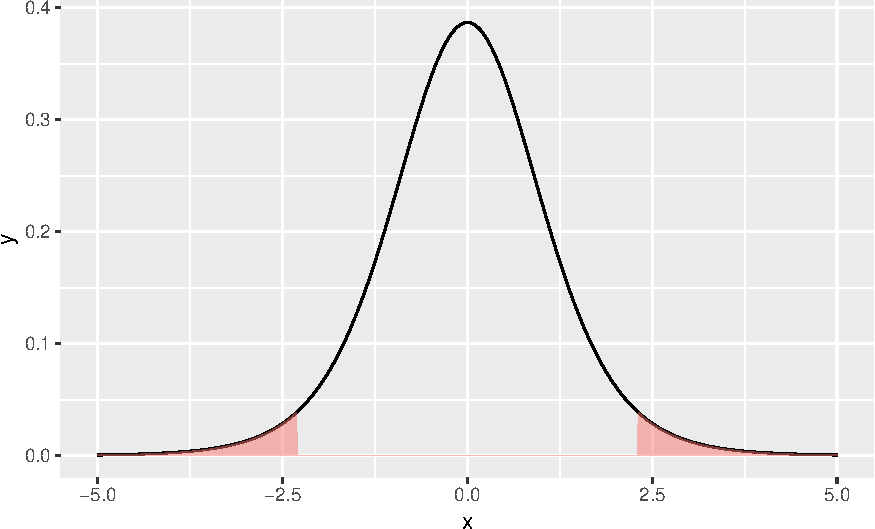
\includegraphics[width=0.7\linewidth]{regression-analysis_files/figure-latex/bjreject-1} 

}

\caption{Rejection region for $\beta_k$}\label{fig:bjreject}
\end{figure}

If we use \texttt{summary()} to \texttt{lm} object, we can get each \(T\) statistic(\texttt{t\ value}), standard error(\texttt{Std.\ Error}), and p-value(\texttt{Pr(\textgreater{}\textbar{}t\textbar{})}). These are the results of partial \(t\)-test.

\begin{Shaded}
\begin{Highlighting}[]
\KeywordTok{summary}\NormalTok{(cem_fit)}
\CommentTok{#> }
\CommentTok{#> Call:}
\CommentTok{#> lm(formula = y ~ ., data = cem)}
\CommentTok{#> }
\CommentTok{#> Residuals:}
\CommentTok{#>    Min     1Q Median     3Q    Max }
\CommentTok{#> -3.175 -1.671  0.251  1.378  3.925 }
\CommentTok{#> }
\CommentTok{#> Coefficients:}
\CommentTok{#>             Estimate Std. Error t value Pr(>|t|)  }
\CommentTok{#> (Intercept)   62.405     70.071    0.89    0.399  }
\CommentTok{#> x1             1.551      0.745    2.08    0.071 .}
\CommentTok{#> x2             0.510      0.724    0.70    0.501  }
\CommentTok{#> x3             0.102      0.755    0.14    0.896  }
\CommentTok{#> x4            -0.144      0.709   -0.20    0.844  }
\CommentTok{#> ---}
\CommentTok{#> Signif. codes:  0 '***' 0.001 '**' 0.01 '*' 0.05 '.' 0.1 ' ' 1}
\CommentTok{#> }
\CommentTok{#> Residual standard error: 2.45 on 8 degrees of freedom}
\CommentTok{#> Multiple R-squared:  0.982,  Adjusted R-squared:  0.974 }
\CommentTok{#> F-statistic:  111 on 4 and 8 DF,  p-value: 4.76e-07}
\end{Highlighting}
\end{Shaded}

If the test is significant, it means that additional contribution of that variable is significant after all other variables are already in the model. This might be understood well with extra sum of squares concept, later.

\hypertarget{prediction-interval-1}{%
\subsection{Prediction interval}\label{prediction-interval-1}}

Consider prediction at \(\mathbf{z} = (1, z_1, \ldots, z_p)^T\). Write

\[C_{\mathbf{z}} := \mathbf{z}^T(X^TX)^{-1}\mathbf{z}\]

\BeginKnitrBlock{theorem}[Prediction or Confidence interval for mean response]
\protect\hypertarget{thm:meanresci}{}{\label{thm:meanresci} \iffalse (Prediction or Confidence interval for mean response) \fi{} }\((1 - \alpha)100\%\) prediction interval for \(\mu_{\mathbf{z}}\) is

\[\bigg[ \hat\mu_{\mathbf{z}} \pm t_{\frac{\alpha}{2}}(n - p - 1)\sqrt{C_{\mathbf{z}}\hat\sigma^2} \bigg]\]
\EndKnitrBlock{theorem}

\BeginKnitrBlock{theorem}[Out-of-sample prediction interval]
\protect\hypertarget{thm:predresci}{}{\label{thm:predresci} \iffalse (Out-of-sample prediction interval) \fi{} }\((1 - \alpha)100\%\) prediction interval for \(Y_{\mathbf{z}}\) is

\[\bigg[ \hat{Y}_{\mathbf{z}} \pm t_{\frac{\alpha}{2}}(n - p - 1)\sqrt{(C_{\mathbf{z}} + 1)\hat\sigma^2} \bigg]\]
\EndKnitrBlock{theorem}

See standard error part of Theorem \ref{thm:meanresci} and Theorem \ref{thm:predresci}. As mentioned, Out of sample prediction interval \emph{always has larger standard error.} This leads to wider interval.

\hypertarget{regression-coefficient-vector}{%
\subsection{Regression coefficient vector}\label{regression-coefficient-vector}}

Now we consider the coefficients simultaneously. For example, \(\boldsymbol\beta= (\beta_0, \beta_1, \ldots, \beta_p)^T\).

Note that

\[\boldsymbol{\hat\beta}- \boldsymbol\beta\sim MVN(\mathbf{0}, \sigma^2(X^TX)^{-1})\]

Then standardization gives

\[\mathbf{Z} \equiv \frac{(X^TX)^{\frac{1}{2}}}{\sigma}(\boldsymbol{\hat\beta}- \boldsymbol\beta) \sim MVN(\mathbf{0}, I)\]

It follows that

\[\mathbf{Z}^T\mathbf{Z} = \frac{(\boldsymbol{\hat\beta}- \boldsymbol\beta)^T X^TX (\boldsymbol{\hat\beta}- \boldsymbol\beta)}{\sigma^2} \sim \chi^2(p + 1)\]

Since \(\frac{SSE}{\sigma^2} \sim \chi^2(n - p - 1)\) and \(\hat\sigma^2 = MSE\),

\begin{equation}
  \begin{split}
    \frac{(\boldsymbol{\hat\beta}- \boldsymbol\beta)^T X^TX (\boldsymbol{\hat\beta}- \boldsymbol\beta)}{\hat\sigma^2 (p + 1)} & = \frac{(X\boldsymbol{\hat\beta}- X\boldsymbol\beta)^T(X\boldsymbol{\hat\beta}- X\boldsymbol\beta)}{MSE} \\
    & = \frac{SSR / (p + 1)}{SSE / (n - p - 1)} \\
    & = F(p + 1, n - p - 1, \delta)
  \end{split}
  \label{eq:bvecdist}
\end{equation}

where \(\delta = \frac{\boldsymbol\beta^TX^T(I - \Pi_{\mathbf{1}})X\boldsymbol\beta}{\sigma^2}\).

\BeginKnitrBlock{corollary}[F-test]
\protect\hypertarget{cor:bvech0}{}{\label{cor:bvech0} \iffalse (F-test) \fi{} }Test \(H_0: \boldsymbol\beta= \mathbf{0} \quad \text{vs} \quad H_1: \boldsymbol\beta\neq \mathbf{0}\). For given data, \(F\)-test computes

\[\frac{(\boldsymbol{\hat\beta}- \boldsymbol\beta)^T X^TX (\boldsymbol{\hat\beta}- \boldsymbol\beta)}{\hat\sigma^2 (p + 1)} = \frac{SSR / (p + 1)}{MSE} \stackrel{H_0}{\sim}F(p + 1, n - p - 1)\]
\EndKnitrBlock{corollary}

From the first part, we can get the confidence region for \(\boldsymbol\beta\).

\BeginKnitrBlock{theorem}[Confidence region]
\protect\hypertarget{thm:bveccr}{}{\label{thm:bveccr} \iffalse (Confidence region) \fi{} }\((1 - \alpha)100\%\) confidence interval for \(\boldsymbol\beta= (\beta_0, \beta_1, \ldots, \beta_p)^T\) is

\[\Big\{ \boldsymbol\beta: (\boldsymbol{\hat\beta}- \boldsymbol\beta)^T X^TX (\boldsymbol{\hat\beta}- \boldsymbol\beta) \le (p + 1)\hat\sigma^2 F_{1 - \alpha}(p + 1, n - p - 1) \Big\}\]
\EndKnitrBlock{theorem}

\BeginKnitrBlock{remark}
\iffalse{} {Remark. } \fi{}The confidence region for the vector \(\boldsymbol\beta\) is the ellipsoid that is centered at \(\boldsymbol{\hat\beta}\). Eigenvectors and eigenvalues of \(X^TX\) determines its orientation and size, respectively. See \citet{Johnson:2013aa} for details.
\EndKnitrBlock{remark}

\texttt{ellipse::ellipse()} has method for \texttt{lm} object. So if you provides the regression object, it will give ellipsoid coordinate as \texttt{matrix}. However, this function only supports two variables. By specifying \texttt{which} argument, you can select which variable to get coordinates. By default, first two variables \texttt{c(1,\ 2)}.

\begin{Shaded}
\begin{Highlighting}[]
\NormalTok{ellipse}\OperatorTok{::}\KeywordTok{ellipse}\NormalTok{(cem_fit) }\OperatorTok\StringTok{ }
\StringTok{  }\KeywordTok{tbl_df}\NormalTok{() }\OperatorTok\StringTok{ }\CommentTok{# change to data frame}
\StringTok{  }\KeywordTok{ggplot}\NormalTok{(}\KeywordTok{aes}\NormalTok{(}\DataTypeTok{x =} \StringTok{`}\DataTypeTok{(Intercept)}\StringTok{`}\NormalTok{, }\DataTypeTok{y =}\NormalTok{ x1)) }\OperatorTok{+}
\StringTok{  }\KeywordTok{geom_path}\NormalTok{()}
\end{Highlighting}
\end{Shaded}

\begin{center}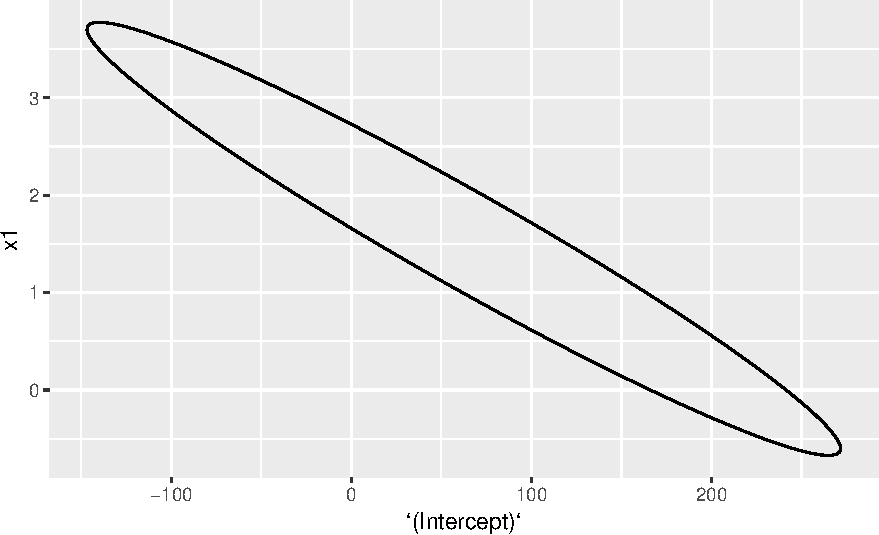
\includegraphics[width=0.7\linewidth]{regression-analysis_files/figure-latex/unnamed-chunk-87-1} \end{center}

Look again corollary \ref{cor:bvech0}. Compare this to ANOVA. Something is different. When testing significance in ANOVA, degrees of freedom of \(SSR\) was \(p\). Because when testing regression relation, we only need \(\beta_1\) to \(\beta_p\), i.e.~\(p\) parameters. How can we do this here?

\hypertarget{regression-coefficient-vector-boldsymbolbeta_a}{%
\subsection{\texorpdfstring{Regression coefficient vector \(\boldsymbol\beta_A\)}{Regression coefficient vector \textbackslash boldsymbol\textbackslash beta\_A}}\label{regression-coefficient-vector-boldsymbolbeta_a}}

Consider \(\boldsymbol\beta_A = (\beta_1, \ldots, \beta_p)^T\). In fact, these tell us significance of variables. We can use \(\mathbb{X}_{A, \perp}\) defined before. From Equation \eqref{eq:orthbeta},

\[\boldsymbol{\hat\beta}_A = (\mathbb{X}_{A,\perp}^T\mathbb{X}_{A,\perp})^{-1}\mathbb{X}_{A,\perp}^T\mathbf{Y}\]

The reason using \(\mathbb{X}_{A, \perp}\) is to decomposing the space orthogonally.

\[
\boldsymbol{\hat\beta}- \boldsymbol\beta= \begin{bmatrix}
  \hat\beta_0 - \beta_0 \\ \hline
  \boldsymbol{\hat\beta}_A - \boldsymbol\beta_A
\end{bmatrix} \sim MVN\Bigg( \begin{bmatrix}
  0 \\ \hline
  \mathbf{0}
\end{bmatrix}, \sigma^2 (X^T X)^{-1} \bigg)
\]

with

\[Var(\boldsymbol{\hat\beta}_A - \boldsymbol\beta_A) = \sigma^2 (\mathbb{X}_{A, \perp}^T\mathbb{X}_{A, \perp})^{-1}\]

\BeginKnitrBlock{theorem}[Confidence region]
\protect\hypertarget{thm:bacr}{}{\label{thm:bacr} \iffalse (Confidence region) \fi{} }\((1 - \alpha)100\%\) confidence interval for \(\boldsymbol\beta_A = (\beta_1, \ldots, \beta_p)^T\) is

\[\Big\{ \boldsymbol\beta_A : (\boldsymbol{\hat\beta}_A - \boldsymbol\beta_A)^T \mathbb{X}_{A, \perp}^T\mathbb{X}_{A, \perp} (\boldsymbol{\hat\beta}_A - \boldsymbol\beta_A) \le p \hat\sigma^2 F_{\alpha}(p, n - p - 1) \Big\}\]

where \(\boldsymbol{\hat\beta}_A = (\mathbb{X}_{A,\perp}^T\mathbb{X}_{A,\perp})^{-1}\mathbb{X}_{A,\perp}^T\mathbf{Y}\)
\EndKnitrBlock{theorem}

This tests the same hypothesis as ANOVA for significance.

\BeginKnitrBlock{remark}
\iffalse{} {Remark. } \fi{}As for \(X\), the confidence region for the vector \(\boldsymbol\beta_A\) is the ellipsoid that is centered at \(\boldsymbol{\hat\beta}_A\). Eigenvectors and eigenvalues of \(\mathbb{X}_{A, \perp}^T\mathbb{X}_{A, \perp}\) determines its orientation and size, respectively.
\EndKnitrBlock{remark}

\hypertarget{nested-models}{%
\section{Nested Models}\label{nested-models}}

We have seen \(t\)-test and \(F\)-test testing \(\beta_j = 0\) and \(\beta_1 = \cdots = \beta_p = 0\), respectively. Here, we generalize the hypothesis in terms of \emph{nested model}. Consider several types of hypothesis.

\BeginKnitrBlock{example}[Examples of three types of hypothesis]
\protect\hypertarget{exm:ftestex}{}{\label{exm:ftestex} \iffalse (Examples of three types of hypothesis) \fi{} }We can test if every coefficient is zero or some coefficient is zero, or just test if coefficients are same not specific value.

\begin{enumerate}
  \item $H_0: \beta_1 = \cdots = \beta_p = 0$
  \item $H_0: \beta_{p - 1} = \beta_p = 0$
  \item $H_0: \beta_{p - 1} = \beta_p$
\end{enumerate}
\EndKnitrBlock{example}

What is the unified approach to these kind of test?

\hypertarget{full-model-and-reduced-model}{%
\subsection{Full model and reduced model}\label{full-model-and-reduced-model}}

To test some forms of \(H_0\), consider two nested model.

\BeginKnitrBlock{definition}[Nested models]
\protect\hypertarget{def:fmrm}{}{\label{def:fmrm} \iffalse (Nested models) \fi{} }We name nested models for the test as follow.

\begin{enumerate}
  \item \textbf{\textit{Full model}} (FM) represents the basic starting model
  \item \textbf{\textit{Reduced model}} (RM) represents the null model under $H_0$
\end{enumerate}
\EndKnitrBlock{definition}

In Example \ref{exm:ftestex}, the basic starting model, i.e.~FM is

\[Y_i = \beta_0 + \beta_1 x_{i1} + \cdots + \beta_p x_{ip} + \epsilon_i, \quad \epsilon_i \stackrel{iid}{\sim}N(0, \sigma^2)\]

See the second case.

\[H_0: \beta_{p - 1} = \beta_p = 0 \qquad \text{vs} \qquad H_1: \beta_{p - 1} \neq 0 \:\text{or}\: \beta_p \neq 0\]

This is equivalent to choosing a model between

\[
\begin{cases}
  FM: Y_i = \beta_0 + \beta_1 x_{i1} + \cdots + \beta_p x_{ip} + \epsilon_i \\
  RM: Y_i = \beta_0 + \beta_1 x_{i1} + \cdots + \beta_{p - 2}x_{i,p-2} + \epsilon_i
\end{cases}
\]

Let us define \(SSR\) and \(SSE\) for each model.

\BeginKnitrBlock{definition}[SS of nested models]
\protect\hypertarget{def:ssfmrm}{}{\label{def:ssfmrm} \iffalse (SS of nested models) \fi{} }For each full model and reduced model, compute \(SSR\) and \(SSE\).

\begin{enumerate}
  \item $SSR(FM)$ regression sum of squares after fitting the FM
  \item $SSE(FM)$ error sum of squares after fitting the FM
  \item $SSR(RM)$ regression sum of squares after fitting the RM
  \item $SSR(RM)$ error sum of squares after fitting the RM
\end{enumerate}
\EndKnitrBlock{definition}

By construction, \(SST = \sum\limits_{i = 1}^n(Y_i - \overline{Y})^2\) does not depend on model. This measures variability when no predictor is used. It jus the variation of a response itself. So it becomes consistent with given data.

\BeginKnitrBlock{remark}
\iffalse{} {Remark. } \fi{}\[SST = SSR(FM) + SSE(FM) = SSR(RM) + SSE(RM)\]

and hence

\[SSE(RM) - SSE(FM) = SSR(FM) - SSR(RM)\]
\EndKnitrBlock{remark}

\(SSE\) indicates a variation that cannot be explained by the model. \(SSR\) represents a variation explained by the model. We can compare each between the two model. If \(SSE(RM) - SSE(FM) = SSR(FM) - SSR(RM)\) is large, then we can think that the full model is explaining given data better than reduced model. Or, \(SSE\) says that full model can explain some parts that reduced model have failed to explained. In terms of \(H_0: RM \:\text{vs}\: H_1: FM\), it can be said that it is a strong evidene supporting FM against RM. In turn, we conclude that \(H_1: \beta_{p - 1} \neq 0 \:\text{or}\: \beta_p \neq 0\) from our first hypothesis set.

\BeginKnitrBlock{conjecture}
\protect\hypertarget{cnj:fmrmdist}{}{\label{cnj:fmrmdist} }\[SSR(FM) - SSR(RM) > c \Leftrightarrow \text{reject}\: H_0\]
\EndKnitrBlock{conjecture}

We can test any hypothesis using RM-FM pair as in Conjecture \ref{cnj:fmrmdist}. The question is

\begin{enumerate}
\def\labelenumi{\arabic{enumi}.}
\tightlist
\item
  What is the distribution of \(SSR(FM) - SSR(RM)\)?
\item
  Then what is \(c\)?
\end{enumerate}

Define two design matrices to build full model and reduced model.

\[
Z_1 := \begin{bmatrix}
  1 & x_{11} & \cdots & x_{1, p - 2} \\
  1 & x_{21} & \cdots & x_{2, p - 2} \\
  \vdots & \vdots & \vdots & \vdots \\
  1 & x_{n1} & \cdots & x_{n,p - 2}
\end{bmatrix}, \quad \text{and} \qquad Z_2 := \begin{bmatrix}
  x_{1, p - 1} & x_{1p} \\
  x_{2, p - 1} & x_{2p} \\
  \vdots & \vdots \\
  x_{n, p - 1} & x_{np}
\end{bmatrix}
\]

\(Z_1\) is a design matrix of reduced model, while \(Z_2\) consists of column vector that was not in \(Z_2\), i.e.~which were specified in \(H_0\). It is intended to make

\[
X^{\ast} = \begin{bmatrix}
  Z_1 \mid Z_2
\end{bmatrix} \in \mathbb{R}^{n \times (p + 1)}
\]

where \(X^{\ast}\) can have different column order with original \(X\). It follows that

\[
\begin{cases}
  FM: \mathbf{Y} = X\boldsymbol\beta_F + \E \\
  RM: \mathbf{Y} = Z_1 \boldsymbol\beta_R + \E
\end{cases}
\]

where \(\boldsymbol\beta_F = (\beta_0, \ldots, \beta_p)^T\) and \(\boldsymbol\beta_R = (\beta_0, \beta_1, \ldots, \beta_{p - 2})^T\). Thus,

\begin{equation}
  \begin{cases}
    SSR(FM) = \mathbf{Y}^T (\Pi_X - \Pi_{\mathbf{1}}) \mathbf{Y} \\
    SSR(RM) = \mathbf{Y}^T (\Pi_{Z_1} - \Pi_{\mathbf{1}}) \mathbf{Y}
  \end{cases}
  \label{eq:ssrfmrm}
\end{equation}

and so

\begin{equation}
  \begin{split}
    SSR(FM) - SSR(RM) & = \mathbf{Y}^T (\Pi_X - \Pi_{\mathbf{1}} - \Pi_{Z_1} + \Pi_{\mathbf{1}}) \mathbf{Y} \\
    & = \mathbf{Y}^T (\Pi_X - \Pi_{Z_1}) \mathbf{Y}
  \end{split}
  \label{eq:fmrmstat}
\end{equation}

\BeginKnitrBlock{lemma}
\protect\hypertarget{lem:ssrfmlem}{}{\label{lem:ssrfmlem} }\(SSR(FM) - SSR(RM)\) satisfies following properties.

\begin{enumerate}
  \item $\Pi_X - \Pi_{Z_1}$ is symmetric and idempotent
  \item $tr(\Pi_X - \Pi_{Z_1}) = (p + 1) - \text{number of parameters in reduced model}$
  \item $SSR(FM) - SSR(RM) \perp\!\!\!\perp SSE(FM)$
\end{enumerate}
\EndKnitrBlock{lemma}

\BeginKnitrBlock{proof}
\iffalse{} {Proof. } \fi{}Propery of prjection implies that

\[\Pi_X \Pi_{Z_1} = \Pi_{Z_1}\]

Note that

\[SSE(FM) = \mathbf{Y}^T (I - \Pi_X) \mathbf{Y}\]

Then

\[(\Pi_X - \Pi_{Z_1})(I - \Pi_X) = 0\]

Hence, \(SSR(FM) - SSR(RM) \perp\!\!\!\perp SSE(FM)\)
\EndKnitrBlock{proof}

Go back to our Example \ref{exm:ftestex}. Denote that \(\Pi_X - \Pi_{Z_1}\) implies that \(R_{p - 1}^2 > R_{p - 2}^2\). It is easy to get

\[tr(\Pi_X - \Pi_{Z_1}) = (p + 1) - (p - 1) = 2\]

Then

\begin{equation}
  \frac{SSR(FM) - SSR(RM)}{\sigma^2} \stackrel{H_0}{\sim}\chi^2(2)
  \label{eq:ssrfmnull}
\end{equation}

From Proposition \ref{prp:ssdist}

\[\frac{SSE(FM)}{\sigma^2} \stackrel{H_0}{\sim}\chi^2(n - p - 1)\]

Since \(SSR(FM) - SSR(RM) \perp\!\!\!\perp SSE(FM)\),

\begin{equation}
  \begin{split}
    \frac{(SSR(FM) - SSR(RM)) / 2}{SSE(FM) / (n - p - 1)} & = \frac{\frac{SSR(FM) - SSR(RM)}{\sigma^2} / 2}{\frac{SSE(FM)}{\sigma^2} / (n - p - 1)} \\
    & \stackrel{H_0}{\sim}F(2, n - p - 1)
  \end{split}
  \label{eq:ssrfmstat}
\end{equation}

Hence, for our

\[H_0: \beta_{p - 1} = \beta_p = 0 \qquad \text{vs} \qquad H_1: \beta_{p - 1} \neq 0 \:\text{or}\: \beta_p \neq 0\]

reject \(H_0\) if \(\frac{(SSR(FM) - SSR(RM)) / 2}{SSE(FM) / (n - p - 1)} > F_{\alpha}(2, n - p - 1)\).

See the numerator part \(SSR(FM) - SSR(RM)\) we have been explored. This can be also written as

\[SSR(X_1, \ldots, X_p) - SSR(X_1, \ldots, X_{p - 2})\]

and this is called \emph{extra sum of squares}.

\hypertarget{extra-sum-of-squares}{%
\subsection{Extra sum of squares}\label{extra-sum-of-squares}}

\BeginKnitrBlock{definition}[Extra sum of squares]
\protect\hypertarget{def:ess}{}{\label{def:ess} \iffalse (Extra sum of squares) \fi{} }Extra sum of squares measures the amount of the additional contribution of variables added after the variables that were already considered. For example,

\[SSR(X_2 \mid X_1) := SSR(X_1, X_2) - SSR(X_1)\]

This measures marginal contribution of \(X_2\) after \(X_1\) is considred. Here, the contribution means marginal increase of \(SSR\). Equivalently, marginal decrease of \(SSE\).
\EndKnitrBlock{definition}

\begin{figure}[H]

{\centering 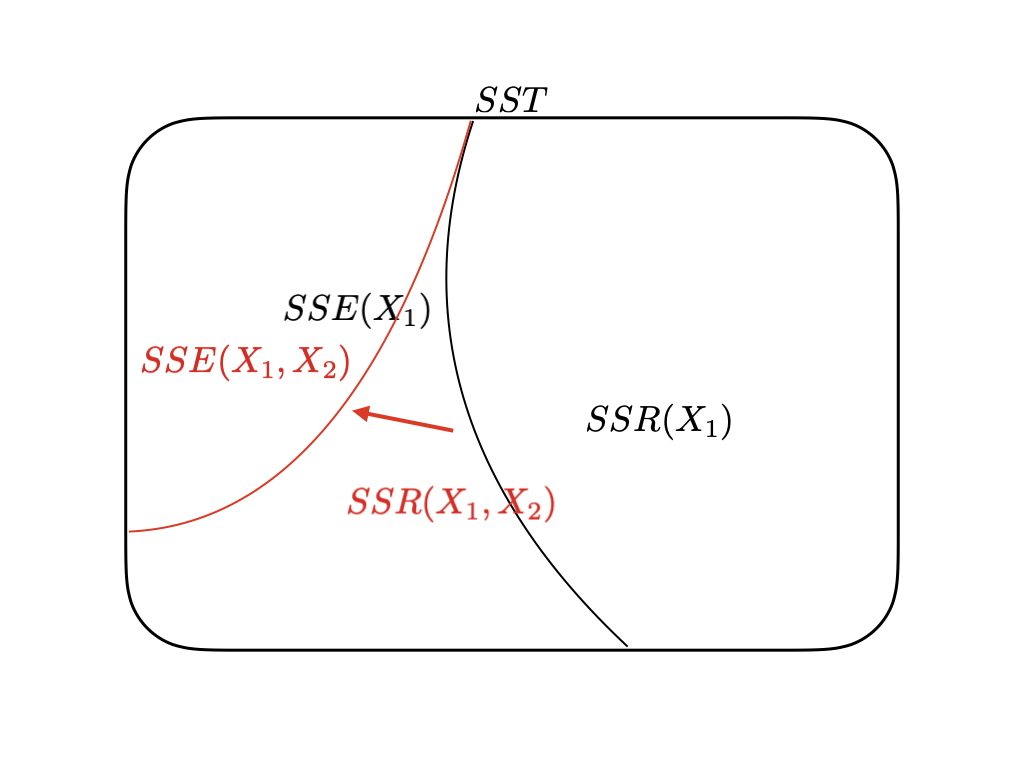
\includegraphics[width=0.7\linewidth]{images/multiple-extrass} 

}

\caption{Extra sum of squares - SSR increases and SSE decreases}\label{fig:essfig}
\end{figure}

Similarly,

\[SSR(X_3, X_4 \mid X_1, X_2) := SSR(X_1, X_2, X_3, X_4) - SSR(X_1, X_2)\]

measures of \(X_3\) and \(X_4\) after \(X_1\) and \(X_2\) are already in the model.

\(SST\) does not change given data. By adding some variables, \(SSR\) increases or \(SSE\) decreases. \emph{We interpret this change as additional contribution of those variables}. If it is large enough, they are significant. Using this idea, we might test any kind of sets of coefficients. Partial \(F\)-test and sequential \(F\)-test are typical forms that we can think of and useful.

\hypertarget{partial-f-test}{%
\subsection{Partial F test}\label{partial-f-test}}

Focus on marginal contribution given that every other predictor is already in the model.

\BeginKnitrBlock{definition}[Partial sum of squares]
\protect\hypertarget{def:pss}{}{\label{def:pss} \iffalse (Partial sum of squares) \fi{} }Partial SS or Type III Sum of squares are following.

\begin{itemize}
  \item $SSR(X_1 \mid X_2, \ldots, X_p)$
  \item $SSR(X_2 \mid X_1, X_3, \ldots, X_p)$
  \item $SSR(X_3 \mid X_1, X_2, X_4, \ldots, X_p)$
  \item $\vdots$
  \item $SSR(X_p \mid X_1, \ldots, X_{p - 1})$
\end{itemize}
\EndKnitrBlock{definition}

\BeginKnitrBlock{remark}
\iffalse{} {Remark. } \fi{}Partial SS satisties following properties.

\begin{enumerate}
  \item $SSR(X_1 \mid X_2, \ldots X_p) + \cdots + SSR(X_p \mid X_1, \ldots, X_{p - 1}) \neq SSR(X_1, \ldots, X_p)$
  \item Partial SS (Type III SS) represents the additional contribution of each predictor after the other predictor variables are considred.
\end{enumerate}
\EndKnitrBlock{remark}

Partial \(F\)-test aims at testing single coefficient.

\[H_0: \beta_j = 0 \qquad \text{vs} \qquad H_1 : \beta_j \neq 0\]

How to make test statistic is same as previous session: using full model and reduced model. Here, one with and without \(\beta_j\).

\begin{equation}
  F_0 = \frac{SSR(X_j \mid X_1, \ldots, X_{j - 1}, X_{j + 1}, \ldots, X_p) / 1}{SSE / (n - p - 1)} \stackrel{H_0}{\sim}F(1, n - p - 1)
  \label{eq:partialstat}
\end{equation}

Hence, reject \(H_0\) if \(F_0 > F_{\alpha}(1, n - p - 1)\). Since the first degrees of freedom is \(1\), we have

\[F_0 = \bigg( \frac{\hat\beta_j}{\widehat{SE}(\hat\beta_j)} \bigg)^2 = T_0^2\]

\BeginKnitrBlock{remark}
\iffalse{} {Remark. } \fi{}Partial \(F\)-test is equivalent to partial \(t\)-test. Both tests the additional contribution of \(X_j\) after the other variables are already considered, not individual significance.
\EndKnitrBlock{remark}

\hypertarget{sequential-f-test}{%
\subsection{Sequential F test}\label{sequential-f-test}}

This sequential \(F\)-test adds variable sequentially.

\BeginKnitrBlock{definition}[Sequential sum of squares]
\protect\hypertarget{def:seqs}{}{\label{def:seqs} \iffalse (Sequential sum of squares) \fi{} }Sequential SS or Type I Sum of squares are following.

\begin{enumerate}
  \item $SSR(X_1)$
  \item $SSR(X_2 \mid X_1)$
  \item $SSR(X_3 \mid X_1, X_2)$
  \item $\vdots$
  \item $SSR(X_p \mid X_1, \ldots, X_{p - 1})$
\end{enumerate}
\EndKnitrBlock{definition}

\BeginKnitrBlock{remark}
\iffalse{} {Remark. } \fi{}Sequential SS satisfies following properties.

\begin{enumerate}
  \item $SSR(X_1) + SSR(X_2 \mid X_1) + \cdots + SSR(X_p \mid X_1, \ldots, X_{p - 1}) = SSR(X_1, \ldots, X_p)$
  \item Sequential SS is useful when we consider nested model. That is, when we know that $X_1$ is the most important, $X_2$ is the second important, and so on.
\end{enumerate}
\EndKnitrBlock{remark}

Following Definition \ref{def:seqs}, start from intercept-only model.

\begin{algorithm}[H] \label{alg:algseq}
  \SetAlgoLined
  \SetKwInOut{Input}{input}
  \SetKwInOut{Output}{output}
  $j \leftarrow 1$\;
  \Repeat{accept $H_0$}{
     $\begin{cases} FM : Y_i = \beta_0 + \cdots + \beta_j x_{1j} + \epsilon_i \\ RM : Y_i = \beta_0 + \ldots + \beta_{j - 1}x_{1, j - 1} + \epsilon_i \end{cases}$\;
    $H_0: \beta_j = 0 (RM) \quad \text{vs} \quad H_1: \beta_j \neq 0 (FM)$\;
    $F_0 = \frac{SSR(X_j \mid X_1, \ldots, X_{j - 1}) / 1}{SSE(X_1, \ldots, X_j) / (n - j - 1)}$\;
    reject $H_0$ if $F_0 > F_{1 - \alpha}(1, n - j - 3)$\;
    $j \leftarrow j + 1$\;
  }
  \Output{accepted model, i.e. final $RM$}
  \caption{Sequential F Test from beginning}
\end{algorithm}

Algorithm \(\ref{alg:algseq}\) shows the logic how to add a variable sequentially. It continues until rejecting \(H_0\). In general form, we can test

\[H_0: \beta_{q + 1} = \beta_{q + 2} = \cdots = \beta_p = 0 \qquad \text{vs} \qquad H_1: \text{not}\: H_0\]

Here, reject \(H_0\) if

\begin{equation}
  \frac{\Big(SSR(X_1, \ldots, X_p) - SSR(X_1, \ldots, X_q)\Big) / (p - q)}{SSE(X_1, \ldots, X_p) / (n - p - 1)} > F_{\alpha}(p - q, n - p - 1)
  \label{eq:seqgen}
\end{equation}

This form of test might be useful when see the significance of categorical predictor. In regression model, quantative predictor is modeled as multiple dummy variables. In this case, we have to see these coefficients all at once and sequential \(F\)-test form might be helpful \citep{Hastie:2013aa}.

\hypertarget{general-linear-hypothesis}{%
\subsection{General linear hypothesis}\label{general-linear-hypothesis}}

See Example \ref{exm:ftestex} again. The third one, \(H_0: \beta_{p - 1} = \beta_p\) can be also tested using \(F\)-test by changing model representation.

\[H_0: \beta_{p - 1} = \beta_p = \alpha \quad \forall \alpha\]

Then null model can be set as

\[Y_i = \beta_0 + \beta_1 x_{i1} + \cdots + \beta_{p - 2} x_{i, p - 2} + \alpha(x_{i, p - 1} + x_{ip}) + \epsilon_i\]

However, there is a more general test procedure: linear combination. For instance, \(\beta_{p - 1} = \beta_p\) can be represented as

\[\beta_{p - 1} - \beta_p = 0 \Leftrightarrow (0, \ldots, 0, 1, -1)^T \boldsymbol\beta= 0\]

Now we analyze this form of hypothesis.

\[H_0: C \boldsymbol\beta= \mathbf{d} \qquad \text{vs} \qquad H_1: C \boldsymbol\beta\neq \mathbf{d}\]

Since \(\hat{\boldsymbol\beta} \sim MVN(\boldsymbol\beta, \sigma^2(X^TX)^{-1})\),

\[C\hat{\boldsymbol\beta} \sim MVN(C \boldsymbol\beta, \sigma^2 C(X^TX)^{-1}C^T)\]

and under \(H_0: C\boldsymbol\beta= \mathbf{d}\),

\[C\hat{\boldsymbol\beta} \stackrel{H_0}{\sim}MVN(\mathbf{d}, \sigma^2 C(X^TX)^{-1}C^T)\]

Set

\[\mathbf{Z} \equiv \frac{1}{\sigma} (C(X^TX)^{-1}C^T)^{-\frac{1}{2}} (C \hat{\boldsymbol\beta} - \mathbf{d}) \stackrel{H_0}{\sim}MVN(\mathbf{0}, I)\]

It follows that

\[\mathbf{Z}^T\mathbf{Z} = \frac{1}{\sigma^2}(C\hat{\boldsymbol\beta} - \mathbf{d})^T(C(X^TX)^{-1}C^T)^{-1}(C\hat{\boldsymbol\beta} - \mathbf{d}) \stackrel{H_0}{\sim}\chi^2(q = rank(C))\]

Since \(SSE \perp\!\!\!\perp\boldsymbol{\hat\beta}\) (See Proposition \ref{prp:ssdist}),

\begin{equation}
  \begin{split}
    \frac{\frac{(C\hat{\boldsymbol\beta} - \mathbf{d})^T(C(X^TX)^{-1}C^T)^{-1}(C\hat{\boldsymbol\beta} - \mathbf{d})}{\sigma^2} / q}{\frac{SSE}{\sigma^2} / (n - p - 1)} & = \frac{(C\hat{\boldsymbol\beta} - \mathbf{d})^T(C(X^TX)^{-1}C^T)^{-1}(C\hat{\boldsymbol\beta} - \mathbf{d}) / q}{\hat\sigma^2} \\
    & \stackrel{H_0}{\sim}F(q, n - p - 1)
  \end{split}
  \label{eq:lincombtest}
\end{equation}

\hypertarget{extra-ss-in-r}{%
\subsection{\texorpdfstring{Extra SS in \texttt{R}}{Extra SS in R}}\label{extra-ss-in-r}}

\texttt{anova.lm()} gives extra sum of squres by default, which is \emph{sequential sum of squares}, i.e.~type I SS.

\begin{Shaded}
\begin{Highlighting}[]
\KeywordTok{anova}\NormalTok{(cem_fit)}
\CommentTok{#> Analysis of Variance Table}
\CommentTok{#> }
\CommentTok{#> Response: y}
\CommentTok{#>           Df Sum Sq Mean Sq F value  Pr(>F)    }
\CommentTok{#> x1         1   1450    1450  242.37 2.9e-07 ***}
\CommentTok{#> x2         1   1208    1208  201.87 5.9e-07 ***}
\CommentTok{#> x3         1     10      10    1.64    0.24    }
\CommentTok{#> x4         1      0       0    0.04    0.84    }
\CommentTok{#> Residuals  8     48       6                    }
\CommentTok{#> ---}
\CommentTok{#> Signif. codes:  0 '***' 0.001 '**' 0.01 '*' 0.05 '.' 0.1 ' ' 1}
\end{Highlighting}
\end{Shaded}

If we change the order,

\begin{Shaded}
\begin{Highlighting}[]
\KeywordTok{anova}\NormalTok{(}\KeywordTok{lm}\NormalTok{(y }\OperatorTok{~}\StringTok{ }\NormalTok{x2 }\OperatorTok{+}\StringTok{ }\NormalTok{x1 }\OperatorTok{+}\StringTok{ }\NormalTok{x3 }\OperatorTok{+}\StringTok{ }\NormalTok{x4, }\DataTypeTok{data =}\NormalTok{ cem))}
\CommentTok{#> Analysis of Variance Table}
\CommentTok{#> }
\CommentTok{#> Response: y}
\CommentTok{#>           Df Sum Sq Mean Sq F value  Pr(>F)    }
\CommentTok{#> x2         1   1809    1809  302.43 1.2e-07 ***}
\CommentTok{#> x1         1    848     848  141.81 2.3e-06 ***}
\CommentTok{#> x3         1     10      10    1.64    0.24    }
\CommentTok{#> x4         1      0       0    0.04    0.84    }
\CommentTok{#> Residuals  8     48       6                    }
\CommentTok{#> ---}
\CommentTok{#> Signif. codes:  0 '***' 0.001 '**' 0.01 '*' 0.05 '.' 0.1 ' ' 1}
\end{Highlighting}
\end{Shaded}

SS differs. To get Type III SS, we can use \texttt{car::Anova()}. This function can compute type II or type III sum of squares. Since it gives type II by default, we should specify \texttt{type\ =\ "III"} or \texttt{type\ =\ 3}.

\begin{Shaded}
\begin{Highlighting}[]
\NormalTok{car}\OperatorTok{::}\KeywordTok{Anova}\NormalTok{(cem_fit, }\DataTypeTok{type =} \DecValTok{3}\NormalTok{)}
\CommentTok{#> Anova Table (Type III tests)}
\CommentTok{#> }
\CommentTok{#> Response: y}
\CommentTok{#>             Sum Sq Df F value Pr(>F)  }
\CommentTok{#> (Intercept)    4.7  1    0.79  0.399  }
\CommentTok{#> x1            26.0  1    4.34  0.071 .}
\CommentTok{#> x2             3.0  1    0.50  0.501  }
\CommentTok{#> x3             0.1  1    0.02  0.896  }
\CommentTok{#> x4             0.2  1    0.04  0.844  }
\CommentTok{#> Residuals     47.9  8                 }
\CommentTok{#> ---}
\CommentTok{#> Signif. codes:  0 '***' 0.001 '**' 0.01 '*' 0.05 '.' 0.1 ' ' 1}
\end{Highlighting}
\end{Shaded}

As base \texttt{anova.lm()}, we can also tidy this object.

\begin{Shaded}
\begin{Highlighting}[]
\NormalTok{car}\OperatorTok{::}\KeywordTok{Anova}\NormalTok{(cem_fit, }\DataTypeTok{type =} \DecValTok{3}\NormalTok{) }\OperatorTok\StringTok{ }
\StringTok{  }\NormalTok{broom}\OperatorTok{::}\KeywordTok{tidy}\NormalTok{()}
\CommentTok{#> # A tibble: 6 x 5}
\CommentTok{#>   term         sumsq    df statistic p.value}
\CommentTok{#>   <chr>        <dbl> <dbl>     <dbl>   <dbl>}
\CommentTok{#> 1 (Intercept)  4.75      1    0.793   0.399 }
\CommentTok{#> 2 x1          26.0       1    4.34    0.0708}
\CommentTok{#> 3 x2           2.97      1    0.497   0.501 }
\CommentTok{#> 4 x3           0.109     1    0.0182  0.896 }
\CommentTok{#> 5 x4           0.247     1    0.0413  0.844 }
\CommentTok{#> 6 Residuals   47.9       8   NA      NA}
\end{Highlighting}
\end{Shaded}

Look p-value of the type III SS, i.e.~partial F-test. Comparing to partial t-test, we can see both are equivalent.

\begin{Shaded}
\begin{Highlighting}[]
\NormalTok{car}\OperatorTok{::}\KeywordTok{Anova}\NormalTok{(cem_fit, }\DataTypeTok{type =} \DecValTok{3}\NormalTok{) }\OperatorTok\StringTok{ }
\StringTok{  }\NormalTok{broom}\OperatorTok{::}\KeywordTok{tidy}\NormalTok{() }\OperatorTok\StringTok{ }
\StringTok{  }\KeywordTok{na.omit}\NormalTok{() }\OperatorTok\StringTok{ }
\StringTok{  }\KeywordTok{select}\NormalTok{(p.value) }\OperatorTok\StringTok{ }
\StringTok{  }\KeywordTok{bind_cols}\NormalTok{(}\DataTypeTok{t_test =}\NormalTok{ broom}\OperatorTok{::}\KeywordTok{tidy}\NormalTok{(cem_fit)}\OperatorTok{$}\NormalTok{p.value)}
\CommentTok{#> # A tibble: 5 x 2}
\CommentTok{#>   p.value t_test}
\CommentTok{#>     <dbl>  <dbl>}
\CommentTok{#> 1  0.399  0.399 }
\CommentTok{#> 2  0.0708 0.0708}
\CommentTok{#> 3  0.501  0.501 }
\CommentTok{#> 4  0.896  0.896 }
\CommentTok{#> 5  0.844  0.844}
\end{Highlighting}
\end{Shaded}

As we can see in the argument of \texttt{car::Anova()}, there are also type II and type IV SS. These are not popular ones, though.

\texttt{car::linearHypothesis()} function peforms test for linear combination. Just specify \(C\) matrix to \texttt{hypothesis.matrix}. If you want additional \(\mathbf{d}\), specify \texttt{rhs}. If this is \texttt{NULL} (by default), test will be done with zero. Try \(H_0: \beta_3 = \beta_4\).

\begin{Shaded}
\begin{Highlighting}[]
\NormalTok{car}\OperatorTok{::}\KeywordTok{linearHypothesis}\NormalTok{(cem_fit, }\DataTypeTok{hypothesis.matrix =} \KeywordTok{c}\NormalTok{(}\DecValTok{0}\NormalTok{, }\DecValTok{0}\NormalTok{, }\DecValTok{0}\NormalTok{, }\DecValTok{1}\NormalTok{, }\DecValTok{-1}\NormalTok{))}
\CommentTok{#> Linear hypothesis test}
\CommentTok{#> }
\CommentTok{#> Hypothesis:}
\CommentTok{#> x3 - x4 = 0}
\CommentTok{#> }
\CommentTok{#> Model 1: restricted model}
\CommentTok{#> Model 2: y ~ x1 + x2 + x3 + x4}
\CommentTok{#> }
\CommentTok{#>   Res.Df  RSS Df Sum of Sq    F Pr(>F)}
\CommentTok{#> 1      9 57.2                         }
\CommentTok{#> 2      8 47.9  1      9.38 1.57   0.25}
\end{Highlighting}
\end{Shaded}

\bibliography{book.bib,packages.bib}


\end{document}
